\documentclass{article}
\usepackage{lmodern}
\usepackage[T1]{fontenc}
\usepackage{shapepar}
\usepackage{microtype}
\usepackage{lipsum}
\usepackage{pgfplots}
\pgfplotsset{compat=1.9}
\usepackage{tikz}
\usetikzlibrary{calc,fit,intersections,folding}
\usepackage{pstricks-add}
\usetikzlibrary{arrows.meta,angles,arrows,quotes,backgrounds}
\usepackage[landscape,a3paper,left=5mm,right=5mm,top=25mm,bottom=25mm]{geometry} % Ränder

\newcommand{\tubecolor}{blue}
\newcommand{\thickness}{0.5mm}
\newcommand{\n}{2mm}


\begin{document}
\thispagestyle{empty}



%123456
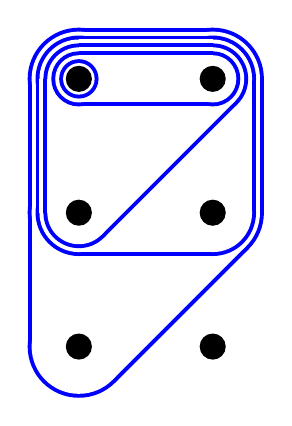
\begin{tikzpicture}
\node[fill] (1) at (0.0, 0.0) [circle] {};
\node[fill] (2) at (1.7, 0.0) [circle] {};
\node[fill] (3) at (0.0, -1.7) [circle] {};
\node[fill] (4) at (1.7, -1.7) [circle] {};
\node[fill] (5) at (0.0, -3.4) [circle] {};
\node[fill] (6) at (1.7, -3.4) [circle] {};
%12345
\begin{scope}[on background layer]
\fill[\tubecolor] (1) circle (\n + 9*\thickness);
\fill[\tubecolor] (2) circle (\n + 9*\thickness);
\fill[\tubecolor] (3) circle (\n + 9*\thickness);
\fill[\tubecolor] (4) circle (\n + 9*\thickness);
\fill[\tubecolor] (5) circle (\n + 9*\thickness);
\draw[\tubecolor] [line width = 2*(\n + 9*\thickness)] (1.center) -- (2.center);
\draw[\tubecolor] [line width = 2*(\n + 9*\thickness)] (1.center) -- (3.center);
\draw[\tubecolor] [line width = 2*(\n + 9*\thickness)] (1.center) -- (4.center);
\draw[\tubecolor] [line width = 2*(\n + 9*\thickness)] (2.center) -- (3.center);
\draw[\tubecolor] [line width = 2*(\n + 9*\thickness)] (2.center) -- (4.center);
\draw[\tubecolor] [line width = 2*(\n + 9*\thickness)] (2.center) -- (5.center);
\draw[\tubecolor] [line width = 2*(\n + 9*\thickness)] (3.center) -- (4.center);
\draw[\tubecolor] [line width = 2*(\n + 9*\thickness)] (3.center) -- (5.center);
\draw[\tubecolor] [line width = 2*(\n + 9*\thickness)] (4.center) -- (5.center);
\draw[white] [line width = 2*(\n + 8*\thickness)] (1.center) -- (2.center);
\draw[white] [line width = 2*(\n + 8*\thickness)] (1.center) -- (3.center);
\draw[white] [line width = 2*(\n + 8*\thickness)] (1.center) -- (4.center);
\draw[white] [line width = 2*(\n + 8*\thickness)] (2.center) -- (3.center);
\draw[white] [line width = 2*(\n + 8*\thickness)] (2.center) -- (4.center);
\draw[white] [line width = 2*(\n + 8*\thickness)] (2.center) -- (5.center);
\draw[white] [line width = 2*(\n + 8*\thickness)] (3.center) -- (4.center);
\draw[white] [line width = 2*(\n + 8*\thickness)] (3.center) -- (5.center);
\draw[white] [line width = 2*(\n + 8*\thickness)] (4.center) -- (5.center);
\fill[white] (1.center) -- (3.center) -- (2.center) -- (1.center);
\fill[white] (2.center) -- (4.center) -- (1.center) -- (2.center);
\fill[white] (1.center) -- (3.center) -- (4.center) -- (1.center);
\fill[white] (2.center) -- (4.center) -- (3.center) -- (2.center);
\fill[white] (3.center) -- (5.center) -- (2.center) -- (3.center);
\fill[white] (2.center) -- (4.center) -- (5.center) -- (2.center);
\fill[white] (3.center) -- (5.center) -- (4.center) -- (3.center);
\fill[white] (1) circle (\n + 8*\thickness);
\fill[white] (2) circle (\n + 8*\thickness);
\fill[white] (3) circle (\n + 8*\thickness);
\fill[white] (4) circle (\n + 8*\thickness);
\fill[white] (5) circle (\n + 8*\thickness);
\end{scope}
%1234
\begin{scope}[on background layer]
\fill[\tubecolor] (1) circle (\n + 7*\thickness);
\fill[\tubecolor] (2) circle (\n + 7*\thickness);
\fill[\tubecolor] (3) circle (\n + 7*\thickness);
\fill[\tubecolor] (4) circle (\n + 7*\thickness);
\draw[\tubecolor] [line width = 2*(\n + 7*\thickness)] (1.center) -- (2.center);
\draw[\tubecolor] [line width = 2*(\n + 7*\thickness)] (1.center) -- (3.center);
\draw[\tubecolor] [line width = 2*(\n + 7*\thickness)] (1.center) -- (4.center);
\draw[\tubecolor] [line width = 2*(\n + 7*\thickness)] (2.center) -- (3.center);
\draw[\tubecolor] [line width = 2*(\n + 7*\thickness)] (2.center) -- (4.center);
\draw[\tubecolor] [line width = 2*(\n + 7*\thickness)] (3.center) -- (4.center);
\draw[white] [line width = 2*(\n + 6*\thickness)] (1.center) -- (2.center);
\draw[white] [line width = 2*(\n + 6*\thickness)] (1.center) -- (3.center);
\draw[white] [line width = 2*(\n + 6*\thickness)] (1.center) -- (4.center);
\draw[white] [line width = 2*(\n + 6*\thickness)] (2.center) -- (3.center);
\draw[white] [line width = 2*(\n + 6*\thickness)] (2.center) -- (4.center);
\draw[white] [line width = 2*(\n + 6*\thickness)] (3.center) -- (4.center);
\fill[white] (1.center) -- (3.center) -- (2.center) -- (1.center);
\fill[white] (2.center) -- (4.center) -- (1.center) -- (2.center);
\fill[white] (1.center) -- (3.center) -- (4.center) -- (1.center);
\fill[white] (2.center) -- (4.center) -- (3.center) -- (2.center);
\fill[white] (1) circle (\n + 6*\thickness);
\fill[white] (2) circle (\n + 6*\thickness);
\fill[white] (3) circle (\n + 6*\thickness);
\fill[white] (4) circle (\n + 6*\thickness);
\end{scope}
%123
\begin{scope}[on background layer]
\fill[\tubecolor] (1) circle (\n + 5*\thickness);
\fill[\tubecolor] (2) circle (\n + 5*\thickness);
\fill[\tubecolor] (3) circle (\n + 5*\thickness);
\draw[\tubecolor] [line width = 2*(\n + 5*\thickness)] (1.center) -- (2.center);
\draw[\tubecolor] [line width = 2*(\n + 5*\thickness)] (1.center) -- (3.center);
\draw[\tubecolor] [line width = 2*(\n + 5*\thickness)] (2.center) -- (3.center);
\draw[white] [line width = 2*(\n + 4*\thickness)] (1.center) -- (2.center);
\draw[white] [line width = 2*(\n + 4*\thickness)] (1.center) -- (3.center);
\draw[white] [line width = 2*(\n + 4*\thickness)] (2.center) -- (3.center);
\fill[white] (1.center) -- (3.center) -- (2.center) -- (1.center);
\fill[white] (1) circle (\n + 4*\thickness);
\fill[white] (2) circle (\n + 4*\thickness);
\fill[white] (3) circle (\n + 4*\thickness);
\end{scope}
%12
\begin{scope}[on background layer]
\fill[\tubecolor] (1) circle (\n + 3*\thickness);
\fill[\tubecolor] (2) circle (\n + 3*\thickness);
\draw[\tubecolor] [line width = 2*(\n + 3*\thickness)] (1.center) -- (2.center);
\draw[white] [line width = 2*(\n + 2*\thickness)] (1.center) -- (2.center);
\fill[white] (1) circle (\n + 2*\thickness);
\fill[white] (2) circle (\n + 2*\thickness);
\end{scope}
%1
\begin{scope}[on background layer]
\fill[\tubecolor] (1) circle (\n + 1*\thickness);
\fill[white] (1) circle (\n + 0*\thickness);
\end{scope}
\end{tikzpicture}
%123546
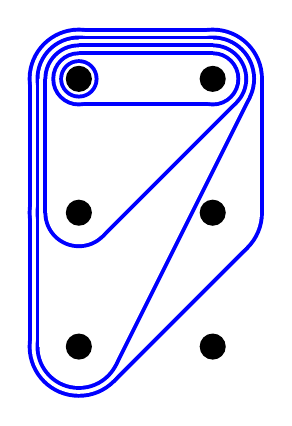
\begin{tikzpicture}
\node[fill] (1) at (0.0, 0.0) [circle] {};
\node[fill] (2) at (1.7, 0.0) [circle] {};
\node[fill] (3) at (0.0, -1.7) [circle] {};
\node[fill] (4) at (1.7, -1.7) [circle] {};
\node[fill] (5) at (0.0, -3.4) [circle] {};
\node[fill] (6) at (1.7, -3.4) [circle] {};
%12345
\begin{scope}[on background layer]
\fill[\tubecolor] (1) circle (\n + 9*\thickness);
\fill[\tubecolor] (2) circle (\n + 9*\thickness);
\fill[\tubecolor] (3) circle (\n + 9*\thickness);
\fill[\tubecolor] (4) circle (\n + 9*\thickness);
\fill[\tubecolor] (5) circle (\n + 9*\thickness);
\draw[\tubecolor] [line width = 2*(\n + 9*\thickness)] (1.center) -- (2.center);
\draw[\tubecolor] [line width = 2*(\n + 9*\thickness)] (1.center) -- (3.center);
\draw[\tubecolor] [line width = 2*(\n + 9*\thickness)] (1.center) -- (4.center);
\draw[\tubecolor] [line width = 2*(\n + 9*\thickness)] (2.center) -- (3.center);
\draw[\tubecolor] [line width = 2*(\n + 9*\thickness)] (2.center) -- (4.center);
\draw[\tubecolor] [line width = 2*(\n + 9*\thickness)] (2.center) -- (5.center);
\draw[\tubecolor] [line width = 2*(\n + 9*\thickness)] (3.center) -- (4.center);
\draw[\tubecolor] [line width = 2*(\n + 9*\thickness)] (3.center) -- (5.center);
\draw[\tubecolor] [line width = 2*(\n + 9*\thickness)] (4.center) -- (5.center);
\draw[white] [line width = 2*(\n + 8*\thickness)] (1.center) -- (2.center);
\draw[white] [line width = 2*(\n + 8*\thickness)] (1.center) -- (3.center);
\draw[white] [line width = 2*(\n + 8*\thickness)] (1.center) -- (4.center);
\draw[white] [line width = 2*(\n + 8*\thickness)] (2.center) -- (3.center);
\draw[white] [line width = 2*(\n + 8*\thickness)] (2.center) -- (4.center);
\draw[white] [line width = 2*(\n + 8*\thickness)] (2.center) -- (5.center);
\draw[white] [line width = 2*(\n + 8*\thickness)] (3.center) -- (4.center);
\draw[white] [line width = 2*(\n + 8*\thickness)] (3.center) -- (5.center);
\draw[white] [line width = 2*(\n + 8*\thickness)] (4.center) -- (5.center);
\fill[white] (1.center) -- (3.center) -- (2.center) -- (1.center);
\fill[white] (2.center) -- (4.center) -- (1.center) -- (2.center);
\fill[white] (1.center) -- (3.center) -- (4.center) -- (1.center);
\fill[white] (2.center) -- (4.center) -- (3.center) -- (2.center);
\fill[white] (3.center) -- (5.center) -- (2.center) -- (3.center);
\fill[white] (2.center) -- (4.center) -- (5.center) -- (2.center);
\fill[white] (3.center) -- (5.center) -- (4.center) -- (3.center);
\fill[white] (1) circle (\n + 8*\thickness);
\fill[white] (2) circle (\n + 8*\thickness);
\fill[white] (3) circle (\n + 8*\thickness);
\fill[white] (4) circle (\n + 8*\thickness);
\fill[white] (5) circle (\n + 8*\thickness);
\end{scope}
%1235
\begin{scope}[on background layer]
\fill[\tubecolor] (1) circle (\n + 7*\thickness);
\fill[\tubecolor] (2) circle (\n + 7*\thickness);
\fill[\tubecolor] (3) circle (\n + 7*\thickness);
\fill[\tubecolor] (5) circle (\n + 7*\thickness);
\draw[\tubecolor] [line width = 2*(\n + 7*\thickness)] (1.center) -- (2.center);
\draw[\tubecolor] [line width = 2*(\n + 7*\thickness)] (1.center) -- (3.center);
\draw[\tubecolor] [line width = 2*(\n + 7*\thickness)] (2.center) -- (3.center);
\draw[\tubecolor] [line width = 2*(\n + 7*\thickness)] (2.center) -- (5.center);
\draw[\tubecolor] [line width = 2*(\n + 7*\thickness)] (3.center) -- (5.center);
\draw[white] [line width = 2*(\n + 6*\thickness)] (1.center) -- (2.center);
\draw[white] [line width = 2*(\n + 6*\thickness)] (1.center) -- (3.center);
\draw[white] [line width = 2*(\n + 6*\thickness)] (2.center) -- (3.center);
\draw[white] [line width = 2*(\n + 6*\thickness)] (2.center) -- (5.center);
\draw[white] [line width = 2*(\n + 6*\thickness)] (3.center) -- (5.center);
\fill[white] (1.center) -- (3.center) -- (2.center) -- (1.center);
\fill[white] (3.center) -- (5.center) -- (2.center) -- (3.center);
\fill[white] (1) circle (\n + 6*\thickness);
\fill[white] (2) circle (\n + 6*\thickness);
\fill[white] (3) circle (\n + 6*\thickness);
\fill[white] (5) circle (\n + 6*\thickness);
\end{scope}
%123
\begin{scope}[on background layer]
\fill[\tubecolor] (1) circle (\n + 5*\thickness);
\fill[\tubecolor] (2) circle (\n + 5*\thickness);
\fill[\tubecolor] (3) circle (\n + 5*\thickness);
\draw[\tubecolor] [line width = 2*(\n + 5*\thickness)] (1.center) -- (2.center);
\draw[\tubecolor] [line width = 2*(\n + 5*\thickness)] (1.center) -- (3.center);
\draw[\tubecolor] [line width = 2*(\n + 5*\thickness)] (2.center) -- (3.center);
\draw[white] [line width = 2*(\n + 4*\thickness)] (1.center) -- (2.center);
\draw[white] [line width = 2*(\n + 4*\thickness)] (1.center) -- (3.center);
\draw[white] [line width = 2*(\n + 4*\thickness)] (2.center) -- (3.center);
\fill[white] (1.center) -- (3.center) -- (2.center) -- (1.center);
\fill[white] (1) circle (\n + 4*\thickness);
\fill[white] (2) circle (\n + 4*\thickness);
\fill[white] (3) circle (\n + 4*\thickness);
\end{scope}
%12
\begin{scope}[on background layer]
\fill[\tubecolor] (1) circle (\n + 3*\thickness);
\fill[\tubecolor] (2) circle (\n + 3*\thickness);
\draw[\tubecolor] [line width = 2*(\n + 3*\thickness)] (1.center) -- (2.center);
\draw[white] [line width = 2*(\n + 2*\thickness)] (1.center) -- (2.center);
\fill[white] (1) circle (\n + 2*\thickness);
\fill[white] (2) circle (\n + 2*\thickness);
\end{scope}
%1
\begin{scope}[on background layer]
\fill[\tubecolor] (1) circle (\n + 1*\thickness);
\fill[white] (1) circle (\n + 0*\thickness);
\end{scope}
\end{tikzpicture}
%125346
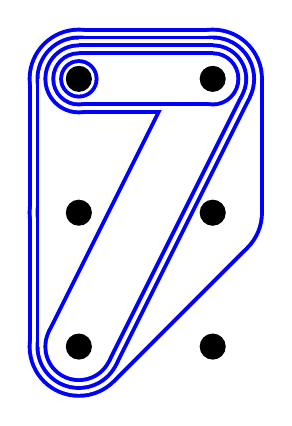
\begin{tikzpicture}
\node[fill] (1) at (0.0, 0.0) [circle] {};
\node[fill] (2) at (1.7, 0.0) [circle] {};
\node[fill] (3) at (0.0, -1.7) [circle] {};
\node[fill] (4) at (1.7, -1.7) [circle] {};
\node[fill] (5) at (0.0, -3.4) [circle] {};
\node[fill] (6) at (1.7, -3.4) [circle] {};
%12345
\begin{scope}[on background layer]
\fill[\tubecolor] (1) circle (\n + 9*\thickness);
\fill[\tubecolor] (2) circle (\n + 9*\thickness);
\fill[\tubecolor] (3) circle (\n + 9*\thickness);
\fill[\tubecolor] (4) circle (\n + 9*\thickness);
\fill[\tubecolor] (5) circle (\n + 9*\thickness);
\draw[\tubecolor] [line width = 2*(\n + 9*\thickness)] (1.center) -- (2.center);
\draw[\tubecolor] [line width = 2*(\n + 9*\thickness)] (1.center) -- (3.center);
\draw[\tubecolor] [line width = 2*(\n + 9*\thickness)] (1.center) -- (4.center);
\draw[\tubecolor] [line width = 2*(\n + 9*\thickness)] (2.center) -- (3.center);
\draw[\tubecolor] [line width = 2*(\n + 9*\thickness)] (2.center) -- (4.center);
\draw[\tubecolor] [line width = 2*(\n + 9*\thickness)] (2.center) -- (5.center);
\draw[\tubecolor] [line width = 2*(\n + 9*\thickness)] (3.center) -- (4.center);
\draw[\tubecolor] [line width = 2*(\n + 9*\thickness)] (3.center) -- (5.center);
\draw[\tubecolor] [line width = 2*(\n + 9*\thickness)] (4.center) -- (5.center);
\draw[white] [line width = 2*(\n + 8*\thickness)] (1.center) -- (2.center);
\draw[white] [line width = 2*(\n + 8*\thickness)] (1.center) -- (3.center);
\draw[white] [line width = 2*(\n + 8*\thickness)] (1.center) -- (4.center);
\draw[white] [line width = 2*(\n + 8*\thickness)] (2.center) -- (3.center);
\draw[white] [line width = 2*(\n + 8*\thickness)] (2.center) -- (4.center);
\draw[white] [line width = 2*(\n + 8*\thickness)] (2.center) -- (5.center);
\draw[white] [line width = 2*(\n + 8*\thickness)] (3.center) -- (4.center);
\draw[white] [line width = 2*(\n + 8*\thickness)] (3.center) -- (5.center);
\draw[white] [line width = 2*(\n + 8*\thickness)] (4.center) -- (5.center);
\fill[white] (1.center) -- (3.center) -- (2.center) -- (1.center);
\fill[white] (2.center) -- (4.center) -- (1.center) -- (2.center);
\fill[white] (1.center) -- (3.center) -- (4.center) -- (1.center);
\fill[white] (2.center) -- (4.center) -- (3.center) -- (2.center);
\fill[white] (3.center) -- (5.center) -- (2.center) -- (3.center);
\fill[white] (2.center) -- (4.center) -- (5.center) -- (2.center);
\fill[white] (3.center) -- (5.center) -- (4.center) -- (3.center);
\fill[white] (1) circle (\n + 8*\thickness);
\fill[white] (2) circle (\n + 8*\thickness);
\fill[white] (3) circle (\n + 8*\thickness);
\fill[white] (4) circle (\n + 8*\thickness);
\fill[white] (5) circle (\n + 8*\thickness);
\end{scope}
%1235
\begin{scope}[on background layer]
\fill[\tubecolor] (1) circle (\n + 7*\thickness);
\fill[\tubecolor] (2) circle (\n + 7*\thickness);
\fill[\tubecolor] (3) circle (\n + 7*\thickness);
\fill[\tubecolor] (5) circle (\n + 7*\thickness);
\draw[\tubecolor] [line width = 2*(\n + 7*\thickness)] (1.center) -- (2.center);
\draw[\tubecolor] [line width = 2*(\n + 7*\thickness)] (1.center) -- (3.center);
\draw[\tubecolor] [line width = 2*(\n + 7*\thickness)] (2.center) -- (3.center);
\draw[\tubecolor] [line width = 2*(\n + 7*\thickness)] (2.center) -- (5.center);
\draw[\tubecolor] [line width = 2*(\n + 7*\thickness)] (3.center) -- (5.center);
\draw[white] [line width = 2*(\n + 6*\thickness)] (1.center) -- (2.center);
\draw[white] [line width = 2*(\n + 6*\thickness)] (1.center) -- (3.center);
\draw[white] [line width = 2*(\n + 6*\thickness)] (2.center) -- (3.center);
\draw[white] [line width = 2*(\n + 6*\thickness)] (2.center) -- (5.center);
\draw[white] [line width = 2*(\n + 6*\thickness)] (3.center) -- (5.center);
\fill[white] (1.center) -- (3.center) -- (2.center) -- (1.center);
\fill[white] (3.center) -- (5.center) -- (2.center) -- (3.center);
\fill[white] (1) circle (\n + 6*\thickness);
\fill[white] (2) circle (\n + 6*\thickness);
\fill[white] (3) circle (\n + 6*\thickness);
\fill[white] (5) circle (\n + 6*\thickness);
\end{scope}
%125
\begin{scope}[on background layer]
\fill[\tubecolor] (1) circle (\n + 5*\thickness);
\fill[\tubecolor] (2) circle (\n + 5*\thickness);
\fill[\tubecolor] (5) circle (\n + 5*\thickness);
\draw[\tubecolor] [line width = 2*(\n + 5*\thickness)] (1.center) -- (2.center);
\draw[\tubecolor] [line width = 2*(\n + 5*\thickness)] (2.center) -- (5.center);
\draw[white] [line width = 2*(\n + 4*\thickness)] (1.center) -- (2.center);
\draw[white] [line width = 2*(\n + 4*\thickness)] (2.center) -- (5.center);
\fill[white] (1) circle (\n + 4*\thickness);
\fill[white] (2) circle (\n + 4*\thickness);
\fill[white] (5) circle (\n + 4*\thickness);
\end{scope}
%12
\begin{scope}[on background layer]
\fill[\tubecolor] (1) circle (\n + 3*\thickness);
\fill[\tubecolor] (2) circle (\n + 3*\thickness);
\draw[\tubecolor] [line width = 2*(\n + 3*\thickness)] (1.center) -- (2.center);
\draw[white] [line width = 2*(\n + 2*\thickness)] (1.center) -- (2.center);
\fill[white] (1) circle (\n + 2*\thickness);
\fill[white] (2) circle (\n + 2*\thickness);
\end{scope}
%1
\begin{scope}[on background layer]
\fill[\tubecolor] (1) circle (\n + 1*\thickness);
\fill[white] (1) circle (\n + 0*\thickness);
\end{scope}
\end{tikzpicture}
%125436
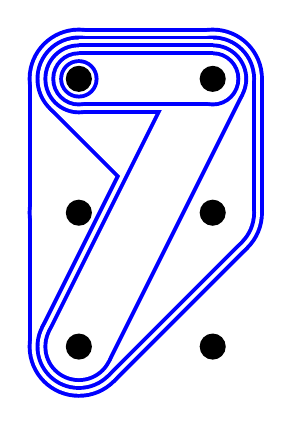
\begin{tikzpicture}
\node[fill] (1) at (0.0, 0.0) [circle] {};
\node[fill] (2) at (1.7, 0.0) [circle] {};
\node[fill] (3) at (0.0, -1.7) [circle] {};
\node[fill] (4) at (1.7, -1.7) [circle] {};
\node[fill] (5) at (0.0, -3.4) [circle] {};
\node[fill] (6) at (1.7, -3.4) [circle] {};
%12345
\begin{scope}[on background layer]
\fill[\tubecolor] (1) circle (\n + 9*\thickness);
\fill[\tubecolor] (2) circle (\n + 9*\thickness);
\fill[\tubecolor] (3) circle (\n + 9*\thickness);
\fill[\tubecolor] (4) circle (\n + 9*\thickness);
\fill[\tubecolor] (5) circle (\n + 9*\thickness);
\draw[\tubecolor] [line width = 2*(\n + 9*\thickness)] (1.center) -- (2.center);
\draw[\tubecolor] [line width = 2*(\n + 9*\thickness)] (1.center) -- (3.center);
\draw[\tubecolor] [line width = 2*(\n + 9*\thickness)] (1.center) -- (4.center);
\draw[\tubecolor] [line width = 2*(\n + 9*\thickness)] (2.center) -- (3.center);
\draw[\tubecolor] [line width = 2*(\n + 9*\thickness)] (2.center) -- (4.center);
\draw[\tubecolor] [line width = 2*(\n + 9*\thickness)] (2.center) -- (5.center);
\draw[\tubecolor] [line width = 2*(\n + 9*\thickness)] (3.center) -- (4.center);
\draw[\tubecolor] [line width = 2*(\n + 9*\thickness)] (3.center) -- (5.center);
\draw[\tubecolor] [line width = 2*(\n + 9*\thickness)] (4.center) -- (5.center);
\draw[white] [line width = 2*(\n + 8*\thickness)] (1.center) -- (2.center);
\draw[white] [line width = 2*(\n + 8*\thickness)] (1.center) -- (3.center);
\draw[white] [line width = 2*(\n + 8*\thickness)] (1.center) -- (4.center);
\draw[white] [line width = 2*(\n + 8*\thickness)] (2.center) -- (3.center);
\draw[white] [line width = 2*(\n + 8*\thickness)] (2.center) -- (4.center);
\draw[white] [line width = 2*(\n + 8*\thickness)] (2.center) -- (5.center);
\draw[white] [line width = 2*(\n + 8*\thickness)] (3.center) -- (4.center);
\draw[white] [line width = 2*(\n + 8*\thickness)] (3.center) -- (5.center);
\draw[white] [line width = 2*(\n + 8*\thickness)] (4.center) -- (5.center);
\fill[white] (1.center) -- (3.center) -- (2.center) -- (1.center);
\fill[white] (2.center) -- (4.center) -- (1.center) -- (2.center);
\fill[white] (1.center) -- (3.center) -- (4.center) -- (1.center);
\fill[white] (2.center) -- (4.center) -- (3.center) -- (2.center);
\fill[white] (3.center) -- (5.center) -- (2.center) -- (3.center);
\fill[white] (2.center) -- (4.center) -- (5.center) -- (2.center);
\fill[white] (3.center) -- (5.center) -- (4.center) -- (3.center);
\fill[white] (1) circle (\n + 8*\thickness);
\fill[white] (2) circle (\n + 8*\thickness);
\fill[white] (3) circle (\n + 8*\thickness);
\fill[white] (4) circle (\n + 8*\thickness);
\fill[white] (5) circle (\n + 8*\thickness);
\end{scope}
%1245
\begin{scope}[on background layer]
\fill[\tubecolor] (1) circle (\n + 7*\thickness);
\fill[\tubecolor] (2) circle (\n + 7*\thickness);
\fill[\tubecolor] (4) circle (\n + 7*\thickness);
\fill[\tubecolor] (5) circle (\n + 7*\thickness);
\draw[\tubecolor] [line width = 2*(\n + 7*\thickness)] (1.center) -- (2.center);
\draw[\tubecolor] [line width = 2*(\n + 7*\thickness)] (1.center) -- (4.center);
\draw[\tubecolor] [line width = 2*(\n + 7*\thickness)] (2.center) -- (4.center);
\draw[\tubecolor] [line width = 2*(\n + 7*\thickness)] (2.center) -- (5.center);
\draw[\tubecolor] [line width = 2*(\n + 7*\thickness)] (4.center) -- (5.center);
\draw[white] [line width = 2*(\n + 6*\thickness)] (1.center) -- (2.center);
\draw[white] [line width = 2*(\n + 6*\thickness)] (1.center) -- (4.center);
\draw[white] [line width = 2*(\n + 6*\thickness)] (2.center) -- (4.center);
\draw[white] [line width = 2*(\n + 6*\thickness)] (2.center) -- (5.center);
\draw[white] [line width = 2*(\n + 6*\thickness)] (4.center) -- (5.center);
\fill[white] (2.center) -- (4.center) -- (1.center) -- (2.center);
\fill[white] (2.center) -- (4.center) -- (5.center) -- (2.center);
\fill[white] (1) circle (\n + 6*\thickness);
\fill[white] (2) circle (\n + 6*\thickness);
\fill[white] (4) circle (\n + 6*\thickness);
\fill[white] (5) circle (\n + 6*\thickness);
\end{scope}
%125
\begin{scope}[on background layer]
\fill[\tubecolor] (1) circle (\n + 5*\thickness);
\fill[\tubecolor] (2) circle (\n + 5*\thickness);
\fill[\tubecolor] (5) circle (\n + 5*\thickness);
\draw[\tubecolor] [line width = 2*(\n + 5*\thickness)] (1.center) -- (2.center);
\draw[\tubecolor] [line width = 2*(\n + 5*\thickness)] (2.center) -- (5.center);
\draw[white] [line width = 2*(\n + 4*\thickness)] (1.center) -- (2.center);
\draw[white] [line width = 2*(\n + 4*\thickness)] (2.center) -- (5.center);
\fill[white] (1) circle (\n + 4*\thickness);
\fill[white] (2) circle (\n + 4*\thickness);
\fill[white] (5) circle (\n + 4*\thickness);
\end{scope}
%12
\begin{scope}[on background layer]
\fill[\tubecolor] (1) circle (\n + 3*\thickness);
\fill[\tubecolor] (2) circle (\n + 3*\thickness);
\draw[\tubecolor] [line width = 2*(\n + 3*\thickness)] (1.center) -- (2.center);
\draw[white] [line width = 2*(\n + 2*\thickness)] (1.center) -- (2.center);
\fill[white] (1) circle (\n + 2*\thickness);
\fill[white] (2) circle (\n + 2*\thickness);
\end{scope}
%1
\begin{scope}[on background layer]
\fill[\tubecolor] (1) circle (\n + 1*\thickness);
\fill[white] (1) circle (\n + 0*\thickness);
\end{scope}
\end{tikzpicture}
%124536
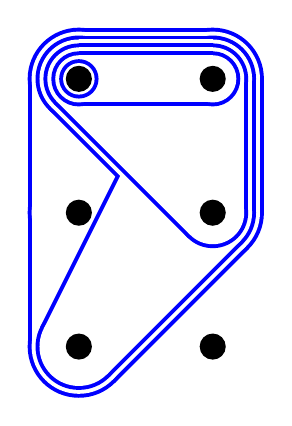
\begin{tikzpicture}
\node[fill] (1) at (0.0, 0.0) [circle] {};
\node[fill] (2) at (1.7, 0.0) [circle] {};
\node[fill] (3) at (0.0, -1.7) [circle] {};
\node[fill] (4) at (1.7, -1.7) [circle] {};
\node[fill] (5) at (0.0, -3.4) [circle] {};
\node[fill] (6) at (1.7, -3.4) [circle] {};
%12345
\begin{scope}[on background layer]
\fill[\tubecolor] (1) circle (\n + 9*\thickness);
\fill[\tubecolor] (2) circle (\n + 9*\thickness);
\fill[\tubecolor] (3) circle (\n + 9*\thickness);
\fill[\tubecolor] (4) circle (\n + 9*\thickness);
\fill[\tubecolor] (5) circle (\n + 9*\thickness);
\draw[\tubecolor] [line width = 2*(\n + 9*\thickness)] (1.center) -- (2.center);
\draw[\tubecolor] [line width = 2*(\n + 9*\thickness)] (1.center) -- (3.center);
\draw[\tubecolor] [line width = 2*(\n + 9*\thickness)] (1.center) -- (4.center);
\draw[\tubecolor] [line width = 2*(\n + 9*\thickness)] (2.center) -- (3.center);
\draw[\tubecolor] [line width = 2*(\n + 9*\thickness)] (2.center) -- (4.center);
\draw[\tubecolor] [line width = 2*(\n + 9*\thickness)] (2.center) -- (5.center);
\draw[\tubecolor] [line width = 2*(\n + 9*\thickness)] (3.center) -- (4.center);
\draw[\tubecolor] [line width = 2*(\n + 9*\thickness)] (3.center) -- (5.center);
\draw[\tubecolor] [line width = 2*(\n + 9*\thickness)] (4.center) -- (5.center);
\draw[white] [line width = 2*(\n + 8*\thickness)] (1.center) -- (2.center);
\draw[white] [line width = 2*(\n + 8*\thickness)] (1.center) -- (3.center);
\draw[white] [line width = 2*(\n + 8*\thickness)] (1.center) -- (4.center);
\draw[white] [line width = 2*(\n + 8*\thickness)] (2.center) -- (3.center);
\draw[white] [line width = 2*(\n + 8*\thickness)] (2.center) -- (4.center);
\draw[white] [line width = 2*(\n + 8*\thickness)] (2.center) -- (5.center);
\draw[white] [line width = 2*(\n + 8*\thickness)] (3.center) -- (4.center);
\draw[white] [line width = 2*(\n + 8*\thickness)] (3.center) -- (5.center);
\draw[white] [line width = 2*(\n + 8*\thickness)] (4.center) -- (5.center);
\fill[white] (1.center) -- (3.center) -- (2.center) -- (1.center);
\fill[white] (2.center) -- (4.center) -- (1.center) -- (2.center);
\fill[white] (1.center) -- (3.center) -- (4.center) -- (1.center);
\fill[white] (2.center) -- (4.center) -- (3.center) -- (2.center);
\fill[white] (3.center) -- (5.center) -- (2.center) -- (3.center);
\fill[white] (2.center) -- (4.center) -- (5.center) -- (2.center);
\fill[white] (3.center) -- (5.center) -- (4.center) -- (3.center);
\fill[white] (1) circle (\n + 8*\thickness);
\fill[white] (2) circle (\n + 8*\thickness);
\fill[white] (3) circle (\n + 8*\thickness);
\fill[white] (4) circle (\n + 8*\thickness);
\fill[white] (5) circle (\n + 8*\thickness);
\end{scope}
%1245
\begin{scope}[on background layer]
\fill[\tubecolor] (1) circle (\n + 7*\thickness);
\fill[\tubecolor] (2) circle (\n + 7*\thickness);
\fill[\tubecolor] (4) circle (\n + 7*\thickness);
\fill[\tubecolor] (5) circle (\n + 7*\thickness);
\draw[\tubecolor] [line width = 2*(\n + 7*\thickness)] (1.center) -- (2.center);
\draw[\tubecolor] [line width = 2*(\n + 7*\thickness)] (1.center) -- (4.center);
\draw[\tubecolor] [line width = 2*(\n + 7*\thickness)] (2.center) -- (4.center);
\draw[\tubecolor] [line width = 2*(\n + 7*\thickness)] (2.center) -- (5.center);
\draw[\tubecolor] [line width = 2*(\n + 7*\thickness)] (4.center) -- (5.center);
\draw[white] [line width = 2*(\n + 6*\thickness)] (1.center) -- (2.center);
\draw[white] [line width = 2*(\n + 6*\thickness)] (1.center) -- (4.center);
\draw[white] [line width = 2*(\n + 6*\thickness)] (2.center) -- (4.center);
\draw[white] [line width = 2*(\n + 6*\thickness)] (2.center) -- (5.center);
\draw[white] [line width = 2*(\n + 6*\thickness)] (4.center) -- (5.center);
\fill[white] (2.center) -- (4.center) -- (1.center) -- (2.center);
\fill[white] (2.center) -- (4.center) -- (5.center) -- (2.center);
\fill[white] (1) circle (\n + 6*\thickness);
\fill[white] (2) circle (\n + 6*\thickness);
\fill[white] (4) circle (\n + 6*\thickness);
\fill[white] (5) circle (\n + 6*\thickness);
\end{scope}
%124
\begin{scope}[on background layer]
\fill[\tubecolor] (1) circle (\n + 5*\thickness);
\fill[\tubecolor] (2) circle (\n + 5*\thickness);
\fill[\tubecolor] (4) circle (\n + 5*\thickness);
\draw[\tubecolor] [line width = 2*(\n + 5*\thickness)] (1.center) -- (2.center);
\draw[\tubecolor] [line width = 2*(\n + 5*\thickness)] (1.center) -- (4.center);
\draw[\tubecolor] [line width = 2*(\n + 5*\thickness)] (2.center) -- (4.center);
\draw[white] [line width = 2*(\n + 4*\thickness)] (1.center) -- (2.center);
\draw[white] [line width = 2*(\n + 4*\thickness)] (1.center) -- (4.center);
\draw[white] [line width = 2*(\n + 4*\thickness)] (2.center) -- (4.center);
\fill[white] (2.center) -- (4.center) -- (1.center) -- (2.center);
\fill[white] (1) circle (\n + 4*\thickness);
\fill[white] (2) circle (\n + 4*\thickness);
\fill[white] (4) circle (\n + 4*\thickness);
\end{scope}
%12
\begin{scope}[on background layer]
\fill[\tubecolor] (1) circle (\n + 3*\thickness);
\fill[\tubecolor] (2) circle (\n + 3*\thickness);
\draw[\tubecolor] [line width = 2*(\n + 3*\thickness)] (1.center) -- (2.center);
\draw[white] [line width = 2*(\n + 2*\thickness)] (1.center) -- (2.center);
\fill[white] (1) circle (\n + 2*\thickness);
\fill[white] (2) circle (\n + 2*\thickness);
\end{scope}
%1
\begin{scope}[on background layer]
\fill[\tubecolor] (1) circle (\n + 1*\thickness);
\fill[white] (1) circle (\n + 0*\thickness);
\end{scope}
\end{tikzpicture}
%142536
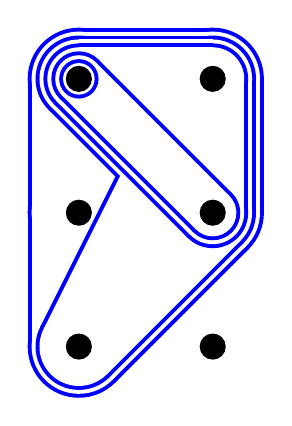
\begin{tikzpicture}
\node[fill] (1) at (0.0, 0.0) [circle] {};
\node[fill] (2) at (1.7, 0.0) [circle] {};
\node[fill] (3) at (0.0, -1.7) [circle] {};
\node[fill] (4) at (1.7, -1.7) [circle] {};
\node[fill] (5) at (0.0, -3.4) [circle] {};
\node[fill] (6) at (1.7, -3.4) [circle] {};
%12345
\begin{scope}[on background layer]
\fill[\tubecolor] (1) circle (\n + 9*\thickness);
\fill[\tubecolor] (2) circle (\n + 9*\thickness);
\fill[\tubecolor] (3) circle (\n + 9*\thickness);
\fill[\tubecolor] (4) circle (\n + 9*\thickness);
\fill[\tubecolor] (5) circle (\n + 9*\thickness);
\draw[\tubecolor] [line width = 2*(\n + 9*\thickness)] (1.center) -- (2.center);
\draw[\tubecolor] [line width = 2*(\n + 9*\thickness)] (1.center) -- (3.center);
\draw[\tubecolor] [line width = 2*(\n + 9*\thickness)] (1.center) -- (4.center);
\draw[\tubecolor] [line width = 2*(\n + 9*\thickness)] (2.center) -- (3.center);
\draw[\tubecolor] [line width = 2*(\n + 9*\thickness)] (2.center) -- (4.center);
\draw[\tubecolor] [line width = 2*(\n + 9*\thickness)] (2.center) -- (5.center);
\draw[\tubecolor] [line width = 2*(\n + 9*\thickness)] (3.center) -- (4.center);
\draw[\tubecolor] [line width = 2*(\n + 9*\thickness)] (3.center) -- (5.center);
\draw[\tubecolor] [line width = 2*(\n + 9*\thickness)] (4.center) -- (5.center);
\draw[white] [line width = 2*(\n + 8*\thickness)] (1.center) -- (2.center);
\draw[white] [line width = 2*(\n + 8*\thickness)] (1.center) -- (3.center);
\draw[white] [line width = 2*(\n + 8*\thickness)] (1.center) -- (4.center);
\draw[white] [line width = 2*(\n + 8*\thickness)] (2.center) -- (3.center);
\draw[white] [line width = 2*(\n + 8*\thickness)] (2.center) -- (4.center);
\draw[white] [line width = 2*(\n + 8*\thickness)] (2.center) -- (5.center);
\draw[white] [line width = 2*(\n + 8*\thickness)] (3.center) -- (4.center);
\draw[white] [line width = 2*(\n + 8*\thickness)] (3.center) -- (5.center);
\draw[white] [line width = 2*(\n + 8*\thickness)] (4.center) -- (5.center);
\fill[white] (1.center) -- (3.center) -- (2.center) -- (1.center);
\fill[white] (2.center) -- (4.center) -- (1.center) -- (2.center);
\fill[white] (1.center) -- (3.center) -- (4.center) -- (1.center);
\fill[white] (2.center) -- (4.center) -- (3.center) -- (2.center);
\fill[white] (3.center) -- (5.center) -- (2.center) -- (3.center);
\fill[white] (2.center) -- (4.center) -- (5.center) -- (2.center);
\fill[white] (3.center) -- (5.center) -- (4.center) -- (3.center);
\fill[white] (1) circle (\n + 8*\thickness);
\fill[white] (2) circle (\n + 8*\thickness);
\fill[white] (3) circle (\n + 8*\thickness);
\fill[white] (4) circle (\n + 8*\thickness);
\fill[white] (5) circle (\n + 8*\thickness);
\end{scope}
%1245
\begin{scope}[on background layer]
\fill[\tubecolor] (1) circle (\n + 7*\thickness);
\fill[\tubecolor] (2) circle (\n + 7*\thickness);
\fill[\tubecolor] (4) circle (\n + 7*\thickness);
\fill[\tubecolor] (5) circle (\n + 7*\thickness);
\draw[\tubecolor] [line width = 2*(\n + 7*\thickness)] (1.center) -- (2.center);
\draw[\tubecolor] [line width = 2*(\n + 7*\thickness)] (1.center) -- (4.center);
\draw[\tubecolor] [line width = 2*(\n + 7*\thickness)] (2.center) -- (4.center);
\draw[\tubecolor] [line width = 2*(\n + 7*\thickness)] (2.center) -- (5.center);
\draw[\tubecolor] [line width = 2*(\n + 7*\thickness)] (4.center) -- (5.center);
\draw[white] [line width = 2*(\n + 6*\thickness)] (1.center) -- (2.center);
\draw[white] [line width = 2*(\n + 6*\thickness)] (1.center) -- (4.center);
\draw[white] [line width = 2*(\n + 6*\thickness)] (2.center) -- (4.center);
\draw[white] [line width = 2*(\n + 6*\thickness)] (2.center) -- (5.center);
\draw[white] [line width = 2*(\n + 6*\thickness)] (4.center) -- (5.center);
\fill[white] (2.center) -- (4.center) -- (1.center) -- (2.center);
\fill[white] (2.center) -- (4.center) -- (5.center) -- (2.center);
\fill[white] (1) circle (\n + 6*\thickness);
\fill[white] (2) circle (\n + 6*\thickness);
\fill[white] (4) circle (\n + 6*\thickness);
\fill[white] (5) circle (\n + 6*\thickness);
\end{scope}
%124
\begin{scope}[on background layer]
\fill[\tubecolor] (1) circle (\n + 5*\thickness);
\fill[\tubecolor] (2) circle (\n + 5*\thickness);
\fill[\tubecolor] (4) circle (\n + 5*\thickness);
\draw[\tubecolor] [line width = 2*(\n + 5*\thickness)] (1.center) -- (2.center);
\draw[\tubecolor] [line width = 2*(\n + 5*\thickness)] (1.center) -- (4.center);
\draw[\tubecolor] [line width = 2*(\n + 5*\thickness)] (2.center) -- (4.center);
\draw[white] [line width = 2*(\n + 4*\thickness)] (1.center) -- (2.center);
\draw[white] [line width = 2*(\n + 4*\thickness)] (1.center) -- (4.center);
\draw[white] [line width = 2*(\n + 4*\thickness)] (2.center) -- (4.center);
\fill[white] (2.center) -- (4.center) -- (1.center) -- (2.center);
\fill[white] (1) circle (\n + 4*\thickness);
\fill[white] (2) circle (\n + 4*\thickness);
\fill[white] (4) circle (\n + 4*\thickness);
\end{scope}
%14
\begin{scope}[on background layer]
\fill[\tubecolor] (1) circle (\n + 3*\thickness);
\fill[\tubecolor] (4) circle (\n + 3*\thickness);
\draw[\tubecolor] [line width = 2*(\n + 3*\thickness)] (1.center) -- (4.center);
\draw[white] [line width = 2*(\n + 2*\thickness)] (1.center) -- (4.center);
\fill[white] (1) circle (\n + 2*\thickness);
\fill[white] (4) circle (\n + 2*\thickness);
\end{scope}
%1
\begin{scope}[on background layer]
\fill[\tubecolor] (1) circle (\n + 1*\thickness);
\fill[white] (1) circle (\n + 0*\thickness);
\end{scope}
\end{tikzpicture}
%145236
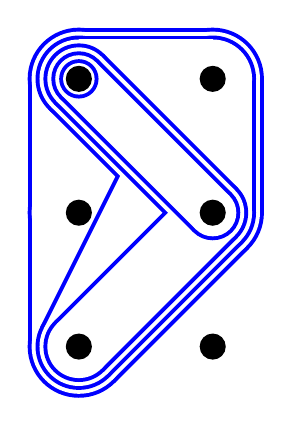
\begin{tikzpicture}
\node[fill] (1) at (0.0, 0.0) [circle] {};
\node[fill] (2) at (1.7, 0.0) [circle] {};
\node[fill] (3) at (0.0, -1.7) [circle] {};
\node[fill] (4) at (1.7, -1.7) [circle] {};
\node[fill] (5) at (0.0, -3.4) [circle] {};
\node[fill] (6) at (1.7, -3.4) [circle] {};
%12345
\begin{scope}[on background layer]
\fill[\tubecolor] (1) circle (\n + 9*\thickness);
\fill[\tubecolor] (2) circle (\n + 9*\thickness);
\fill[\tubecolor] (3) circle (\n + 9*\thickness);
\fill[\tubecolor] (4) circle (\n + 9*\thickness);
\fill[\tubecolor] (5) circle (\n + 9*\thickness);
\draw[\tubecolor] [line width = 2*(\n + 9*\thickness)] (1.center) -- (2.center);
\draw[\tubecolor] [line width = 2*(\n + 9*\thickness)] (1.center) -- (3.center);
\draw[\tubecolor] [line width = 2*(\n + 9*\thickness)] (1.center) -- (4.center);
\draw[\tubecolor] [line width = 2*(\n + 9*\thickness)] (2.center) -- (3.center);
\draw[\tubecolor] [line width = 2*(\n + 9*\thickness)] (2.center) -- (4.center);
\draw[\tubecolor] [line width = 2*(\n + 9*\thickness)] (2.center) -- (5.center);
\draw[\tubecolor] [line width = 2*(\n + 9*\thickness)] (3.center) -- (4.center);
\draw[\tubecolor] [line width = 2*(\n + 9*\thickness)] (3.center) -- (5.center);
\draw[\tubecolor] [line width = 2*(\n + 9*\thickness)] (4.center) -- (5.center);
\draw[white] [line width = 2*(\n + 8*\thickness)] (1.center) -- (2.center);
\draw[white] [line width = 2*(\n + 8*\thickness)] (1.center) -- (3.center);
\draw[white] [line width = 2*(\n + 8*\thickness)] (1.center) -- (4.center);
\draw[white] [line width = 2*(\n + 8*\thickness)] (2.center) -- (3.center);
\draw[white] [line width = 2*(\n + 8*\thickness)] (2.center) -- (4.center);
\draw[white] [line width = 2*(\n + 8*\thickness)] (2.center) -- (5.center);
\draw[white] [line width = 2*(\n + 8*\thickness)] (3.center) -- (4.center);
\draw[white] [line width = 2*(\n + 8*\thickness)] (3.center) -- (5.center);
\draw[white] [line width = 2*(\n + 8*\thickness)] (4.center) -- (5.center);
\fill[white] (1.center) -- (3.center) -- (2.center) -- (1.center);
\fill[white] (2.center) -- (4.center) -- (1.center) -- (2.center);
\fill[white] (1.center) -- (3.center) -- (4.center) -- (1.center);
\fill[white] (2.center) -- (4.center) -- (3.center) -- (2.center);
\fill[white] (3.center) -- (5.center) -- (2.center) -- (3.center);
\fill[white] (2.center) -- (4.center) -- (5.center) -- (2.center);
\fill[white] (3.center) -- (5.center) -- (4.center) -- (3.center);
\fill[white] (1) circle (\n + 8*\thickness);
\fill[white] (2) circle (\n + 8*\thickness);
\fill[white] (3) circle (\n + 8*\thickness);
\fill[white] (4) circle (\n + 8*\thickness);
\fill[white] (5) circle (\n + 8*\thickness);
\end{scope}
%1245
\begin{scope}[on background layer]
\fill[\tubecolor] (1) circle (\n + 7*\thickness);
\fill[\tubecolor] (2) circle (\n + 7*\thickness);
\fill[\tubecolor] (4) circle (\n + 7*\thickness);
\fill[\tubecolor] (5) circle (\n + 7*\thickness);
\draw[\tubecolor] [line width = 2*(\n + 7*\thickness)] (1.center) -- (2.center);
\draw[\tubecolor] [line width = 2*(\n + 7*\thickness)] (1.center) -- (4.center);
\draw[\tubecolor] [line width = 2*(\n + 7*\thickness)] (2.center) -- (4.center);
\draw[\tubecolor] [line width = 2*(\n + 7*\thickness)] (2.center) -- (5.center);
\draw[\tubecolor] [line width = 2*(\n + 7*\thickness)] (4.center) -- (5.center);
\draw[white] [line width = 2*(\n + 6*\thickness)] (1.center) -- (2.center);
\draw[white] [line width = 2*(\n + 6*\thickness)] (1.center) -- (4.center);
\draw[white] [line width = 2*(\n + 6*\thickness)] (2.center) -- (4.center);
\draw[white] [line width = 2*(\n + 6*\thickness)] (2.center) -- (5.center);
\draw[white] [line width = 2*(\n + 6*\thickness)] (4.center) -- (5.center);
\fill[white] (2.center) -- (4.center) -- (1.center) -- (2.center);
\fill[white] (2.center) -- (4.center) -- (5.center) -- (2.center);
\fill[white] (1) circle (\n + 6*\thickness);
\fill[white] (2) circle (\n + 6*\thickness);
\fill[white] (4) circle (\n + 6*\thickness);
\fill[white] (5) circle (\n + 6*\thickness);
\end{scope}
%145
\begin{scope}[on background layer]
\fill[\tubecolor] (1) circle (\n + 5*\thickness);
\fill[\tubecolor] (4) circle (\n + 5*\thickness);
\fill[\tubecolor] (5) circle (\n + 5*\thickness);
\draw[\tubecolor] [line width = 2*(\n + 5*\thickness)] (1.center) -- (4.center);
\draw[\tubecolor] [line width = 2*(\n + 5*\thickness)] (4.center) -- (5.center);
\draw[white] [line width = 2*(\n + 4*\thickness)] (1.center) -- (4.center);
\draw[white] [line width = 2*(\n + 4*\thickness)] (4.center) -- (5.center);
\fill[white] (1) circle (\n + 4*\thickness);
\fill[white] (4) circle (\n + 4*\thickness);
\fill[white] (5) circle (\n + 4*\thickness);
\end{scope}
%14
\begin{scope}[on background layer]
\fill[\tubecolor] (1) circle (\n + 3*\thickness);
\fill[\tubecolor] (4) circle (\n + 3*\thickness);
\draw[\tubecolor] [line width = 2*(\n + 3*\thickness)] (1.center) -- (4.center);
\draw[white] [line width = 2*(\n + 2*\thickness)] (1.center) -- (4.center);
\fill[white] (1) circle (\n + 2*\thickness);
\fill[white] (4) circle (\n + 2*\thickness);
\end{scope}
%1
\begin{scope}[on background layer]
\fill[\tubecolor] (1) circle (\n + 1*\thickness);
\fill[white] (1) circle (\n + 0*\thickness);
\end{scope}
\end{tikzpicture}
%145326
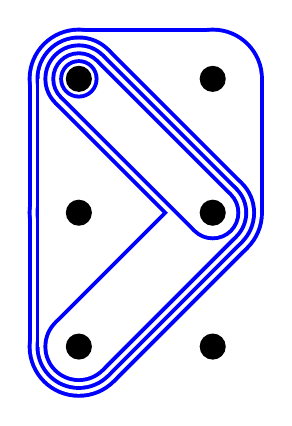
\begin{tikzpicture}
\node[fill] (1) at (0.0, 0.0) [circle] {};
\node[fill] (2) at (1.7, 0.0) [circle] {};
\node[fill] (3) at (0.0, -1.7) [circle] {};
\node[fill] (4) at (1.7, -1.7) [circle] {};
\node[fill] (5) at (0.0, -3.4) [circle] {};
\node[fill] (6) at (1.7, -3.4) [circle] {};
%12345
\begin{scope}[on background layer]
\fill[\tubecolor] (1) circle (\n + 9*\thickness);
\fill[\tubecolor] (2) circle (\n + 9*\thickness);
\fill[\tubecolor] (3) circle (\n + 9*\thickness);
\fill[\tubecolor] (4) circle (\n + 9*\thickness);
\fill[\tubecolor] (5) circle (\n + 9*\thickness);
\draw[\tubecolor] [line width = 2*(\n + 9*\thickness)] (1.center) -- (2.center);
\draw[\tubecolor] [line width = 2*(\n + 9*\thickness)] (1.center) -- (3.center);
\draw[\tubecolor] [line width = 2*(\n + 9*\thickness)] (1.center) -- (4.center);
\draw[\tubecolor] [line width = 2*(\n + 9*\thickness)] (2.center) -- (3.center);
\draw[\tubecolor] [line width = 2*(\n + 9*\thickness)] (2.center) -- (4.center);
\draw[\tubecolor] [line width = 2*(\n + 9*\thickness)] (2.center) -- (5.center);
\draw[\tubecolor] [line width = 2*(\n + 9*\thickness)] (3.center) -- (4.center);
\draw[\tubecolor] [line width = 2*(\n + 9*\thickness)] (3.center) -- (5.center);
\draw[\tubecolor] [line width = 2*(\n + 9*\thickness)] (4.center) -- (5.center);
\draw[white] [line width = 2*(\n + 8*\thickness)] (1.center) -- (2.center);
\draw[white] [line width = 2*(\n + 8*\thickness)] (1.center) -- (3.center);
\draw[white] [line width = 2*(\n + 8*\thickness)] (1.center) -- (4.center);
\draw[white] [line width = 2*(\n + 8*\thickness)] (2.center) -- (3.center);
\draw[white] [line width = 2*(\n + 8*\thickness)] (2.center) -- (4.center);
\draw[white] [line width = 2*(\n + 8*\thickness)] (2.center) -- (5.center);
\draw[white] [line width = 2*(\n + 8*\thickness)] (3.center) -- (4.center);
\draw[white] [line width = 2*(\n + 8*\thickness)] (3.center) -- (5.center);
\draw[white] [line width = 2*(\n + 8*\thickness)] (4.center) -- (5.center);
\fill[white] (1.center) -- (3.center) -- (2.center) -- (1.center);
\fill[white] (2.center) -- (4.center) -- (1.center) -- (2.center);
\fill[white] (1.center) -- (3.center) -- (4.center) -- (1.center);
\fill[white] (2.center) -- (4.center) -- (3.center) -- (2.center);
\fill[white] (3.center) -- (5.center) -- (2.center) -- (3.center);
\fill[white] (2.center) -- (4.center) -- (5.center) -- (2.center);
\fill[white] (3.center) -- (5.center) -- (4.center) -- (3.center);
\fill[white] (1) circle (\n + 8*\thickness);
\fill[white] (2) circle (\n + 8*\thickness);
\fill[white] (3) circle (\n + 8*\thickness);
\fill[white] (4) circle (\n + 8*\thickness);
\fill[white] (5) circle (\n + 8*\thickness);
\end{scope}
%1345
\begin{scope}[on background layer]
\fill[\tubecolor] (1) circle (\n + 7*\thickness);
\fill[\tubecolor] (3) circle (\n + 7*\thickness);
\fill[\tubecolor] (4) circle (\n + 7*\thickness);
\fill[\tubecolor] (5) circle (\n + 7*\thickness);
\draw[\tubecolor] [line width = 2*(\n + 7*\thickness)] (1.center) -- (3.center);
\draw[\tubecolor] [line width = 2*(\n + 7*\thickness)] (1.center) -- (4.center);
\draw[\tubecolor] [line width = 2*(\n + 7*\thickness)] (3.center) -- (4.center);
\draw[\tubecolor] [line width = 2*(\n + 7*\thickness)] (3.center) -- (5.center);
\draw[\tubecolor] [line width = 2*(\n + 7*\thickness)] (4.center) -- (5.center);
\draw[white] [line width = 2*(\n + 6*\thickness)] (1.center) -- (3.center);
\draw[white] [line width = 2*(\n + 6*\thickness)] (1.center) -- (4.center);
\draw[white] [line width = 2*(\n + 6*\thickness)] (3.center) -- (4.center);
\draw[white] [line width = 2*(\n + 6*\thickness)] (3.center) -- (5.center);
\draw[white] [line width = 2*(\n + 6*\thickness)] (4.center) -- (5.center);
\fill[white] (1.center) -- (3.center) -- (4.center) -- (1.center);
\fill[white] (3.center) -- (5.center) -- (4.center) -- (3.center);
\fill[white] (1) circle (\n + 6*\thickness);
\fill[white] (3) circle (\n + 6*\thickness);
\fill[white] (4) circle (\n + 6*\thickness);
\fill[white] (5) circle (\n + 6*\thickness);
\end{scope}
%145
\begin{scope}[on background layer]
\fill[\tubecolor] (1) circle (\n + 5*\thickness);
\fill[\tubecolor] (4) circle (\n + 5*\thickness);
\fill[\tubecolor] (5) circle (\n + 5*\thickness);
\draw[\tubecolor] [line width = 2*(\n + 5*\thickness)] (1.center) -- (4.center);
\draw[\tubecolor] [line width = 2*(\n + 5*\thickness)] (4.center) -- (5.center);
\draw[white] [line width = 2*(\n + 4*\thickness)] (1.center) -- (4.center);
\draw[white] [line width = 2*(\n + 4*\thickness)] (4.center) -- (5.center);
\fill[white] (1) circle (\n + 4*\thickness);
\fill[white] (4) circle (\n + 4*\thickness);
\fill[white] (5) circle (\n + 4*\thickness);
\end{scope}
%14
\begin{scope}[on background layer]
\fill[\tubecolor] (1) circle (\n + 3*\thickness);
\fill[\tubecolor] (4) circle (\n + 3*\thickness);
\draw[\tubecolor] [line width = 2*(\n + 3*\thickness)] (1.center) -- (4.center);
\draw[white] [line width = 2*(\n + 2*\thickness)] (1.center) -- (4.center);
\fill[white] (1) circle (\n + 2*\thickness);
\fill[white] (4) circle (\n + 2*\thickness);
\end{scope}
%1
\begin{scope}[on background layer]
\fill[\tubecolor] (1) circle (\n + 1*\thickness);
\fill[white] (1) circle (\n + 0*\thickness);
\end{scope}
\end{tikzpicture}
%143526
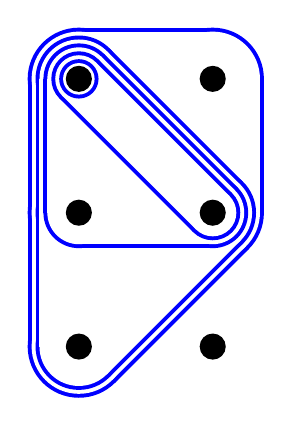
\begin{tikzpicture}
\node[fill] (1) at (0.0, 0.0) [circle] {};
\node[fill] (2) at (1.7, 0.0) [circle] {};
\node[fill] (3) at (0.0, -1.7) [circle] {};
\node[fill] (4) at (1.7, -1.7) [circle] {};
\node[fill] (5) at (0.0, -3.4) [circle] {};
\node[fill] (6) at (1.7, -3.4) [circle] {};
%12345
\begin{scope}[on background layer]
\fill[\tubecolor] (1) circle (\n + 9*\thickness);
\fill[\tubecolor] (2) circle (\n + 9*\thickness);
\fill[\tubecolor] (3) circle (\n + 9*\thickness);
\fill[\tubecolor] (4) circle (\n + 9*\thickness);
\fill[\tubecolor] (5) circle (\n + 9*\thickness);
\draw[\tubecolor] [line width = 2*(\n + 9*\thickness)] (1.center) -- (2.center);
\draw[\tubecolor] [line width = 2*(\n + 9*\thickness)] (1.center) -- (3.center);
\draw[\tubecolor] [line width = 2*(\n + 9*\thickness)] (1.center) -- (4.center);
\draw[\tubecolor] [line width = 2*(\n + 9*\thickness)] (2.center) -- (3.center);
\draw[\tubecolor] [line width = 2*(\n + 9*\thickness)] (2.center) -- (4.center);
\draw[\tubecolor] [line width = 2*(\n + 9*\thickness)] (2.center) -- (5.center);
\draw[\tubecolor] [line width = 2*(\n + 9*\thickness)] (3.center) -- (4.center);
\draw[\tubecolor] [line width = 2*(\n + 9*\thickness)] (3.center) -- (5.center);
\draw[\tubecolor] [line width = 2*(\n + 9*\thickness)] (4.center) -- (5.center);
\draw[white] [line width = 2*(\n + 8*\thickness)] (1.center) -- (2.center);
\draw[white] [line width = 2*(\n + 8*\thickness)] (1.center) -- (3.center);
\draw[white] [line width = 2*(\n + 8*\thickness)] (1.center) -- (4.center);
\draw[white] [line width = 2*(\n + 8*\thickness)] (2.center) -- (3.center);
\draw[white] [line width = 2*(\n + 8*\thickness)] (2.center) -- (4.center);
\draw[white] [line width = 2*(\n + 8*\thickness)] (2.center) -- (5.center);
\draw[white] [line width = 2*(\n + 8*\thickness)] (3.center) -- (4.center);
\draw[white] [line width = 2*(\n + 8*\thickness)] (3.center) -- (5.center);
\draw[white] [line width = 2*(\n + 8*\thickness)] (4.center) -- (5.center);
\fill[white] (1.center) -- (3.center) -- (2.center) -- (1.center);
\fill[white] (2.center) -- (4.center) -- (1.center) -- (2.center);
\fill[white] (1.center) -- (3.center) -- (4.center) -- (1.center);
\fill[white] (2.center) -- (4.center) -- (3.center) -- (2.center);
\fill[white] (3.center) -- (5.center) -- (2.center) -- (3.center);
\fill[white] (2.center) -- (4.center) -- (5.center) -- (2.center);
\fill[white] (3.center) -- (5.center) -- (4.center) -- (3.center);
\fill[white] (1) circle (\n + 8*\thickness);
\fill[white] (2) circle (\n + 8*\thickness);
\fill[white] (3) circle (\n + 8*\thickness);
\fill[white] (4) circle (\n + 8*\thickness);
\fill[white] (5) circle (\n + 8*\thickness);
\end{scope}
%1345
\begin{scope}[on background layer]
\fill[\tubecolor] (1) circle (\n + 7*\thickness);
\fill[\tubecolor] (3) circle (\n + 7*\thickness);
\fill[\tubecolor] (4) circle (\n + 7*\thickness);
\fill[\tubecolor] (5) circle (\n + 7*\thickness);
\draw[\tubecolor] [line width = 2*(\n + 7*\thickness)] (1.center) -- (3.center);
\draw[\tubecolor] [line width = 2*(\n + 7*\thickness)] (1.center) -- (4.center);
\draw[\tubecolor] [line width = 2*(\n + 7*\thickness)] (3.center) -- (4.center);
\draw[\tubecolor] [line width = 2*(\n + 7*\thickness)] (3.center) -- (5.center);
\draw[\tubecolor] [line width = 2*(\n + 7*\thickness)] (4.center) -- (5.center);
\draw[white] [line width = 2*(\n + 6*\thickness)] (1.center) -- (3.center);
\draw[white] [line width = 2*(\n + 6*\thickness)] (1.center) -- (4.center);
\draw[white] [line width = 2*(\n + 6*\thickness)] (3.center) -- (4.center);
\draw[white] [line width = 2*(\n + 6*\thickness)] (3.center) -- (5.center);
\draw[white] [line width = 2*(\n + 6*\thickness)] (4.center) -- (5.center);
\fill[white] (1.center) -- (3.center) -- (4.center) -- (1.center);
\fill[white] (3.center) -- (5.center) -- (4.center) -- (3.center);
\fill[white] (1) circle (\n + 6*\thickness);
\fill[white] (3) circle (\n + 6*\thickness);
\fill[white] (4) circle (\n + 6*\thickness);
\fill[white] (5) circle (\n + 6*\thickness);
\end{scope}
%134
\begin{scope}[on background layer]
\fill[\tubecolor] (1) circle (\n + 5*\thickness);
\fill[\tubecolor] (3) circle (\n + 5*\thickness);
\fill[\tubecolor] (4) circle (\n + 5*\thickness);
\draw[\tubecolor] [line width = 2*(\n + 5*\thickness)] (1.center) -- (3.center);
\draw[\tubecolor] [line width = 2*(\n + 5*\thickness)] (1.center) -- (4.center);
\draw[\tubecolor] [line width = 2*(\n + 5*\thickness)] (3.center) -- (4.center);
\draw[white] [line width = 2*(\n + 4*\thickness)] (1.center) -- (3.center);
\draw[white] [line width = 2*(\n + 4*\thickness)] (1.center) -- (4.center);
\draw[white] [line width = 2*(\n + 4*\thickness)] (3.center) -- (4.center);
\fill[white] (1.center) -- (3.center) -- (4.center) -- (1.center);
\fill[white] (1) circle (\n + 4*\thickness);
\fill[white] (3) circle (\n + 4*\thickness);
\fill[white] (4) circle (\n + 4*\thickness);
\end{scope}
%14
\begin{scope}[on background layer]
\fill[\tubecolor] (1) circle (\n + 3*\thickness);
\fill[\tubecolor] (4) circle (\n + 3*\thickness);
\draw[\tubecolor] [line width = 2*(\n + 3*\thickness)] (1.center) -- (4.center);
\draw[white] [line width = 2*(\n + 2*\thickness)] (1.center) -- (4.center);
\fill[white] (1) circle (\n + 2*\thickness);
\fill[white] (4) circle (\n + 2*\thickness);
\end{scope}
%1
\begin{scope}[on background layer]
\fill[\tubecolor] (1) circle (\n + 1*\thickness);
\fill[white] (1) circle (\n + 0*\thickness);
\end{scope}
\end{tikzpicture}


%143562
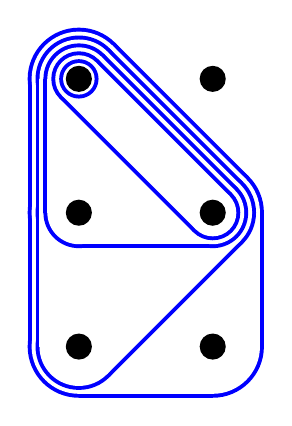
\begin{tikzpicture}
\node[fill] (1) at (0.0, 0.0) [circle] {};
\node[fill] (2) at (1.7, 0.0) [circle] {};
\node[fill] (3) at (0.0, -1.7) [circle] {};
\node[fill] (4) at (1.7, -1.7) [circle] {};
\node[fill] (5) at (0.0, -3.4) [circle] {};
\node[fill] (6) at (1.7, -3.4) [circle] {};
%13456
\begin{scope}[on background layer]
\fill[\tubecolor] (1) circle (\n + 9*\thickness);
\fill[\tubecolor] (3) circle (\n + 9*\thickness);
\fill[\tubecolor] (4) circle (\n + 9*\thickness);
\fill[\tubecolor] (5) circle (\n + 9*\thickness);
\fill[\tubecolor] (6) circle (\n + 9*\thickness);
\draw[\tubecolor] [line width = 2*(\n + 9*\thickness)] (1.center) -- (3.center);
\draw[\tubecolor] [line width = 2*(\n + 9*\thickness)] (1.center) -- (4.center);
\draw[\tubecolor] [line width = 2*(\n + 9*\thickness)] (1.center) -- (6.center);
\draw[\tubecolor] [line width = 2*(\n + 9*\thickness)] (3.center) -- (4.center);
\draw[\tubecolor] [line width = 2*(\n + 9*\thickness)] (3.center) -- (5.center);
\draw[\tubecolor] [line width = 2*(\n + 9*\thickness)] (3.center) -- (6.center);
\draw[\tubecolor] [line width = 2*(\n + 9*\thickness)] (4.center) -- (5.center);
\draw[\tubecolor] [line width = 2*(\n + 9*\thickness)] (4.center) -- (6.center);
\draw[\tubecolor] [line width = 2*(\n + 9*\thickness)] (5.center) -- (6.center);
\draw[white] [line width = 2*(\n + 8*\thickness)] (1.center) -- (3.center);
\draw[white] [line width = 2*(\n + 8*\thickness)] (1.center) -- (4.center);
\draw[white] [line width = 2*(\n + 8*\thickness)] (1.center) -- (6.center);
\draw[white] [line width = 2*(\n + 8*\thickness)] (3.center) -- (4.center);
\draw[white] [line width = 2*(\n + 8*\thickness)] (3.center) -- (5.center);
\draw[white] [line width = 2*(\n + 8*\thickness)] (3.center) -- (6.center);
\draw[white] [line width = 2*(\n + 8*\thickness)] (4.center) -- (5.center);
\draw[white] [line width = 2*(\n + 8*\thickness)] (4.center) -- (6.center);
\draw[white] [line width = 2*(\n + 8*\thickness)] (5.center) -- (6.center);
\fill[white] (1.center) -- (3.center) -- (4.center) -- (1.center);
\fill[white] (1.center) -- (3.center) -- (6.center) -- (1.center);
\fill[white] (4.center) -- (6.center) -- (1.center) -- (4.center);
\fill[white] (3.center) -- (5.center) -- (4.center) -- (3.center);
\fill[white] (4.center) -- (6.center) -- (3.center) -- (4.center);
\fill[white] (3.center) -- (5.center) -- (6.center) -- (3.center);
\fill[white] (4.center) -- (6.center) -- (5.center) -- (4.center);
\fill[white] (1) circle (\n + 8*\thickness);
\fill[white] (3) circle (\n + 8*\thickness);
\fill[white] (4) circle (\n + 8*\thickness);
\fill[white] (5) circle (\n + 8*\thickness);
\fill[white] (6) circle (\n + 8*\thickness);
\end{scope}
%1345
\begin{scope}[on background layer]
\fill[\tubecolor] (1) circle (\n + 7*\thickness);
\fill[\tubecolor] (3) circle (\n + 7*\thickness);
\fill[\tubecolor] (4) circle (\n + 7*\thickness);
\fill[\tubecolor] (5) circle (\n + 7*\thickness);
\draw[\tubecolor] [line width = 2*(\n + 7*\thickness)] (1.center) -- (3.center);
\draw[\tubecolor] [line width = 2*(\n + 7*\thickness)] (1.center) -- (4.center);
\draw[\tubecolor] [line width = 2*(\n + 7*\thickness)] (3.center) -- (4.center);
\draw[\tubecolor] [line width = 2*(\n + 7*\thickness)] (3.center) -- (5.center);
\draw[\tubecolor] [line width = 2*(\n + 7*\thickness)] (4.center) -- (5.center);
\draw[white] [line width = 2*(\n + 6*\thickness)] (1.center) -- (3.center);
\draw[white] [line width = 2*(\n + 6*\thickness)] (1.center) -- (4.center);
\draw[white] [line width = 2*(\n + 6*\thickness)] (3.center) -- (4.center);
\draw[white] [line width = 2*(\n + 6*\thickness)] (3.center) -- (5.center);
\draw[white] [line width = 2*(\n + 6*\thickness)] (4.center) -- (5.center);
\fill[white] (1.center) -- (3.center) -- (4.center) -- (1.center);
\fill[white] (3.center) -- (5.center) -- (4.center) -- (3.center);
\fill[white] (1) circle (\n + 6*\thickness);
\fill[white] (3) circle (\n + 6*\thickness);
\fill[white] (4) circle (\n + 6*\thickness);
\fill[white] (5) circle (\n + 6*\thickness);
\end{scope}
%134
\begin{scope}[on background layer]
\fill[\tubecolor] (1) circle (\n + 5*\thickness);
\fill[\tubecolor] (3) circle (\n + 5*\thickness);
\fill[\tubecolor] (4) circle (\n + 5*\thickness);
\draw[\tubecolor] [line width = 2*(\n + 5*\thickness)] (1.center) -- (3.center);
\draw[\tubecolor] [line width = 2*(\n + 5*\thickness)] (1.center) -- (4.center);
\draw[\tubecolor] [line width = 2*(\n + 5*\thickness)] (3.center) -- (4.center);
\draw[white] [line width = 2*(\n + 4*\thickness)] (1.center) -- (3.center);
\draw[white] [line width = 2*(\n + 4*\thickness)] (1.center) -- (4.center);
\draw[white] [line width = 2*(\n + 4*\thickness)] (3.center) -- (4.center);
\fill[white] (1.center) -- (3.center) -- (4.center) -- (1.center);
\fill[white] (1) circle (\n + 4*\thickness);
\fill[white] (3) circle (\n + 4*\thickness);
\fill[white] (4) circle (\n + 4*\thickness);
\end{scope}
%14
\begin{scope}[on background layer]
\fill[\tubecolor] (1) circle (\n + 3*\thickness);
\fill[\tubecolor] (4) circle (\n + 3*\thickness);
\draw[\tubecolor] [line width = 2*(\n + 3*\thickness)] (1.center) -- (4.center);
\draw[white] [line width = 2*(\n + 2*\thickness)] (1.center) -- (4.center);
\fill[white] (1) circle (\n + 2*\thickness);
\fill[white] (4) circle (\n + 2*\thickness);
\end{scope}
%1
\begin{scope}[on background layer]
\fill[\tubecolor] (1) circle (\n + 1*\thickness);
\fill[white] (1) circle (\n + 0*\thickness);
\end{scope}
\end{tikzpicture}
%143652
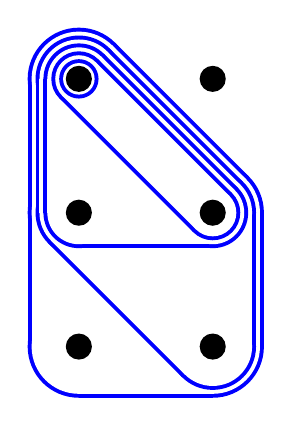
\begin{tikzpicture}
\node[fill] (1) at (0.0, 0.0) [circle] {};
\node[fill] (2) at (1.7, 0.0) [circle] {};
\node[fill] (3) at (0.0, -1.7) [circle] {};
\node[fill] (4) at (1.7, -1.7) [circle] {};
\node[fill] (5) at (0.0, -3.4) [circle] {};
\node[fill] (6) at (1.7, -3.4) [circle] {};
%13456
\begin{scope}[on background layer]
\fill[\tubecolor] (1) circle (\n + 9*\thickness);
\fill[\tubecolor] (3) circle (\n + 9*\thickness);
\fill[\tubecolor] (4) circle (\n + 9*\thickness);
\fill[\tubecolor] (5) circle (\n + 9*\thickness);
\fill[\tubecolor] (6) circle (\n + 9*\thickness);
\draw[\tubecolor] [line width = 2*(\n + 9*\thickness)] (1.center) -- (3.center);
\draw[\tubecolor] [line width = 2*(\n + 9*\thickness)] (1.center) -- (4.center);
\draw[\tubecolor] [line width = 2*(\n + 9*\thickness)] (1.center) -- (6.center);
\draw[\tubecolor] [line width = 2*(\n + 9*\thickness)] (3.center) -- (4.center);
\draw[\tubecolor] [line width = 2*(\n + 9*\thickness)] (3.center) -- (5.center);
\draw[\tubecolor] [line width = 2*(\n + 9*\thickness)] (3.center) -- (6.center);
\draw[\tubecolor] [line width = 2*(\n + 9*\thickness)] (4.center) -- (5.center);
\draw[\tubecolor] [line width = 2*(\n + 9*\thickness)] (4.center) -- (6.center);
\draw[\tubecolor] [line width = 2*(\n + 9*\thickness)] (5.center) -- (6.center);
\draw[white] [line width = 2*(\n + 8*\thickness)] (1.center) -- (3.center);
\draw[white] [line width = 2*(\n + 8*\thickness)] (1.center) -- (4.center);
\draw[white] [line width = 2*(\n + 8*\thickness)] (1.center) -- (6.center);
\draw[white] [line width = 2*(\n + 8*\thickness)] (3.center) -- (4.center);
\draw[white] [line width = 2*(\n + 8*\thickness)] (3.center) -- (5.center);
\draw[white] [line width = 2*(\n + 8*\thickness)] (3.center) -- (6.center);
\draw[white] [line width = 2*(\n + 8*\thickness)] (4.center) -- (5.center);
\draw[white] [line width = 2*(\n + 8*\thickness)] (4.center) -- (6.center);
\draw[white] [line width = 2*(\n + 8*\thickness)] (5.center) -- (6.center);
\fill[white] (1.center) -- (3.center) -- (4.center) -- (1.center);
\fill[white] (1.center) -- (3.center) -- (6.center) -- (1.center);
\fill[white] (4.center) -- (6.center) -- (1.center) -- (4.center);
\fill[white] (3.center) -- (5.center) -- (4.center) -- (3.center);
\fill[white] (4.center) -- (6.center) -- (3.center) -- (4.center);
\fill[white] (3.center) -- (5.center) -- (6.center) -- (3.center);
\fill[white] (4.center) -- (6.center) -- (5.center) -- (4.center);
\fill[white] (1) circle (\n + 8*\thickness);
\fill[white] (3) circle (\n + 8*\thickness);
\fill[white] (4) circle (\n + 8*\thickness);
\fill[white] (5) circle (\n + 8*\thickness);
\fill[white] (6) circle (\n + 8*\thickness);
\end{scope}
%1346
\begin{scope}[on background layer]
\fill[\tubecolor] (1) circle (\n + 7*\thickness);
\fill[\tubecolor] (3) circle (\n + 7*\thickness);
\fill[\tubecolor] (4) circle (\n + 7*\thickness);
\fill[\tubecolor] (6) circle (\n + 7*\thickness);
\draw[\tubecolor] [line width = 2*(\n + 7*\thickness)] (1.center) -- (3.center);
\draw[\tubecolor] [line width = 2*(\n + 7*\thickness)] (1.center) -- (4.center);
\draw[\tubecolor] [line width = 2*(\n + 7*\thickness)] (1.center) -- (6.center);
\draw[\tubecolor] [line width = 2*(\n + 7*\thickness)] (3.center) -- (4.center);
\draw[\tubecolor] [line width = 2*(\n + 7*\thickness)] (3.center) -- (6.center);
\draw[\tubecolor] [line width = 2*(\n + 7*\thickness)] (4.center) -- (6.center);
\draw[white] [line width = 2*(\n + 6*\thickness)] (1.center) -- (3.center);
\draw[white] [line width = 2*(\n + 6*\thickness)] (1.center) -- (4.center);
\draw[white] [line width = 2*(\n + 6*\thickness)] (1.center) -- (6.center);
\draw[white] [line width = 2*(\n + 6*\thickness)] (3.center) -- (4.center);
\draw[white] [line width = 2*(\n + 6*\thickness)] (3.center) -- (6.center);
\draw[white] [line width = 2*(\n + 6*\thickness)] (4.center) -- (6.center);
\fill[white] (1.center) -- (3.center) -- (4.center) -- (1.center);
\fill[white] (1.center) -- (3.center) -- (6.center) -- (1.center);
\fill[white] (4.center) -- (6.center) -- (1.center) -- (4.center);
\fill[white] (4.center) -- (6.center) -- (3.center) -- (4.center);
\fill[white] (1) circle (\n + 6*\thickness);
\fill[white] (3) circle (\n + 6*\thickness);
\fill[white] (4) circle (\n + 6*\thickness);
\fill[white] (6) circle (\n + 6*\thickness);
\end{scope}
%134
\begin{scope}[on background layer]
\fill[\tubecolor] (1) circle (\n + 5*\thickness);
\fill[\tubecolor] (3) circle (\n + 5*\thickness);
\fill[\tubecolor] (4) circle (\n + 5*\thickness);
\draw[\tubecolor] [line width = 2*(\n + 5*\thickness)] (1.center) -- (3.center);
\draw[\tubecolor] [line width = 2*(\n + 5*\thickness)] (1.center) -- (4.center);
\draw[\tubecolor] [line width = 2*(\n + 5*\thickness)] (3.center) -- (4.center);
\draw[white] [line width = 2*(\n + 4*\thickness)] (1.center) -- (3.center);
\draw[white] [line width = 2*(\n + 4*\thickness)] (1.center) -- (4.center);
\draw[white] [line width = 2*(\n + 4*\thickness)] (3.center) -- (4.center);
\fill[white] (1.center) -- (3.center) -- (4.center) -- (1.center);
\fill[white] (1) circle (\n + 4*\thickness);
\fill[white] (3) circle (\n + 4*\thickness);
\fill[white] (4) circle (\n + 4*\thickness);
\end{scope}
%14
\begin{scope}[on background layer]
\fill[\tubecolor] (1) circle (\n + 3*\thickness);
\fill[\tubecolor] (4) circle (\n + 3*\thickness);
\draw[\tubecolor] [line width = 2*(\n + 3*\thickness)] (1.center) -- (4.center);
\draw[white] [line width = 2*(\n + 2*\thickness)] (1.center) -- (4.center);
\fill[white] (1) circle (\n + 2*\thickness);
\fill[white] (4) circle (\n + 2*\thickness);
\end{scope}
%1
\begin{scope}[on background layer]
\fill[\tubecolor] (1) circle (\n + 1*\thickness);
\fill[white] (1) circle (\n + 0*\thickness);
\end{scope}
\end{tikzpicture}
%146352
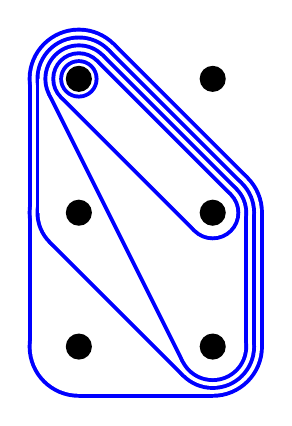
\begin{tikzpicture}
\node[fill] (1) at (0.0, 0.0) [circle] {};
\node[fill] (2) at (1.7, 0.0) [circle] {};
\node[fill] (3) at (0.0, -1.7) [circle] {};
\node[fill] (4) at (1.7, -1.7) [circle] {};
\node[fill] (5) at (0.0, -3.4) [circle] {};
\node[fill] (6) at (1.7, -3.4) [circle] {};
%13456
\begin{scope}[on background layer]
\fill[\tubecolor] (1) circle (\n + 9*\thickness);
\fill[\tubecolor] (3) circle (\n + 9*\thickness);
\fill[\tubecolor] (4) circle (\n + 9*\thickness);
\fill[\tubecolor] (5) circle (\n + 9*\thickness);
\fill[\tubecolor] (6) circle (\n + 9*\thickness);
\draw[\tubecolor] [line width = 2*(\n + 9*\thickness)] (1.center) -- (3.center);
\draw[\tubecolor] [line width = 2*(\n + 9*\thickness)] (1.center) -- (4.center);
\draw[\tubecolor] [line width = 2*(\n + 9*\thickness)] (1.center) -- (6.center);
\draw[\tubecolor] [line width = 2*(\n + 9*\thickness)] (3.center) -- (4.center);
\draw[\tubecolor] [line width = 2*(\n + 9*\thickness)] (3.center) -- (5.center);
\draw[\tubecolor] [line width = 2*(\n + 9*\thickness)] (3.center) -- (6.center);
\draw[\tubecolor] [line width = 2*(\n + 9*\thickness)] (4.center) -- (5.center);
\draw[\tubecolor] [line width = 2*(\n + 9*\thickness)] (4.center) -- (6.center);
\draw[\tubecolor] [line width = 2*(\n + 9*\thickness)] (5.center) -- (6.center);
\draw[white] [line width = 2*(\n + 8*\thickness)] (1.center) -- (3.center);
\draw[white] [line width = 2*(\n + 8*\thickness)] (1.center) -- (4.center);
\draw[white] [line width = 2*(\n + 8*\thickness)] (1.center) -- (6.center);
\draw[white] [line width = 2*(\n + 8*\thickness)] (3.center) -- (4.center);
\draw[white] [line width = 2*(\n + 8*\thickness)] (3.center) -- (5.center);
\draw[white] [line width = 2*(\n + 8*\thickness)] (3.center) -- (6.center);
\draw[white] [line width = 2*(\n + 8*\thickness)] (4.center) -- (5.center);
\draw[white] [line width = 2*(\n + 8*\thickness)] (4.center) -- (6.center);
\draw[white] [line width = 2*(\n + 8*\thickness)] (5.center) -- (6.center);
\fill[white] (1.center) -- (3.center) -- (4.center) -- (1.center);
\fill[white] (1.center) -- (3.center) -- (6.center) -- (1.center);
\fill[white] (4.center) -- (6.center) -- (1.center) -- (4.center);
\fill[white] (3.center) -- (5.center) -- (4.center) -- (3.center);
\fill[white] (4.center) -- (6.center) -- (3.center) -- (4.center);
\fill[white] (3.center) -- (5.center) -- (6.center) -- (3.center);
\fill[white] (4.center) -- (6.center) -- (5.center) -- (4.center);
\fill[white] (1) circle (\n + 8*\thickness);
\fill[white] (3) circle (\n + 8*\thickness);
\fill[white] (4) circle (\n + 8*\thickness);
\fill[white] (5) circle (\n + 8*\thickness);
\fill[white] (6) circle (\n + 8*\thickness);
\end{scope}
%1346
\begin{scope}[on background layer]
\fill[\tubecolor] (1) circle (\n + 7*\thickness);
\fill[\tubecolor] (3) circle (\n + 7*\thickness);
\fill[\tubecolor] (4) circle (\n + 7*\thickness);
\fill[\tubecolor] (6) circle (\n + 7*\thickness);
\draw[\tubecolor] [line width = 2*(\n + 7*\thickness)] (1.center) -- (3.center);
\draw[\tubecolor] [line width = 2*(\n + 7*\thickness)] (1.center) -- (4.center);
\draw[\tubecolor] [line width = 2*(\n + 7*\thickness)] (1.center) -- (6.center);
\draw[\tubecolor] [line width = 2*(\n + 7*\thickness)] (3.center) -- (4.center);
\draw[\tubecolor] [line width = 2*(\n + 7*\thickness)] (3.center) -- (6.center);
\draw[\tubecolor] [line width = 2*(\n + 7*\thickness)] (4.center) -- (6.center);
\draw[white] [line width = 2*(\n + 6*\thickness)] (1.center) -- (3.center);
\draw[white] [line width = 2*(\n + 6*\thickness)] (1.center) -- (4.center);
\draw[white] [line width = 2*(\n + 6*\thickness)] (1.center) -- (6.center);
\draw[white] [line width = 2*(\n + 6*\thickness)] (3.center) -- (4.center);
\draw[white] [line width = 2*(\n + 6*\thickness)] (3.center) -- (6.center);
\draw[white] [line width = 2*(\n + 6*\thickness)] (4.center) -- (6.center);
\fill[white] (1.center) -- (3.center) -- (4.center) -- (1.center);
\fill[white] (1.center) -- (3.center) -- (6.center) -- (1.center);
\fill[white] (4.center) -- (6.center) -- (1.center) -- (4.center);
\fill[white] (4.center) -- (6.center) -- (3.center) -- (4.center);
\fill[white] (1) circle (\n + 6*\thickness);
\fill[white] (3) circle (\n + 6*\thickness);
\fill[white] (4) circle (\n + 6*\thickness);
\fill[white] (6) circle (\n + 6*\thickness);
\end{scope}
%146
\begin{scope}[on background layer]
\fill[\tubecolor] (1) circle (\n + 5*\thickness);
\fill[\tubecolor] (4) circle (\n + 5*\thickness);
\fill[\tubecolor] (6) circle (\n + 5*\thickness);
\draw[\tubecolor] [line width = 2*(\n + 5*\thickness)] (1.center) -- (4.center);
\draw[\tubecolor] [line width = 2*(\n + 5*\thickness)] (1.center) -- (6.center);
\draw[\tubecolor] [line width = 2*(\n + 5*\thickness)] (4.center) -- (6.center);
\draw[white] [line width = 2*(\n + 4*\thickness)] (1.center) -- (4.center);
\draw[white] [line width = 2*(\n + 4*\thickness)] (1.center) -- (6.center);
\draw[white] [line width = 2*(\n + 4*\thickness)] (4.center) -- (6.center);
\fill[white] (4.center) -- (6.center) -- (1.center) -- (4.center);
\fill[white] (1) circle (\n + 4*\thickness);
\fill[white] (4) circle (\n + 4*\thickness);
\fill[white] (6) circle (\n + 4*\thickness);
\end{scope}
%14
\begin{scope}[on background layer]
\fill[\tubecolor] (1) circle (\n + 3*\thickness);
\fill[\tubecolor] (4) circle (\n + 3*\thickness);
\draw[\tubecolor] [line width = 2*(\n + 3*\thickness)] (1.center) -- (4.center);
\draw[white] [line width = 2*(\n + 2*\thickness)] (1.center) -- (4.center);
\fill[white] (1) circle (\n + 2*\thickness);
\fill[white] (4) circle (\n + 2*\thickness);
\end{scope}
%1
\begin{scope}[on background layer]
\fill[\tubecolor] (1) circle (\n + 1*\thickness);
\fill[white] (1) circle (\n + 0*\thickness);
\end{scope}
\end{tikzpicture}
%164352
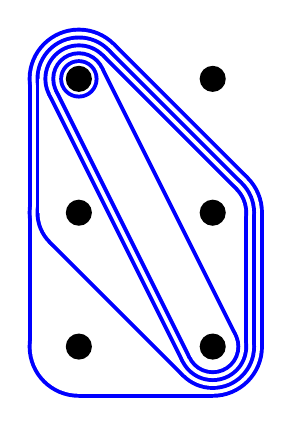
\begin{tikzpicture}
\node[fill] (1) at (0.0, 0.0) [circle] {};
\node[fill] (2) at (1.7, 0.0) [circle] {};
\node[fill] (3) at (0.0, -1.7) [circle] {};
\node[fill] (4) at (1.7, -1.7) [circle] {};
\node[fill] (5) at (0.0, -3.4) [circle] {};
\node[fill] (6) at (1.7, -3.4) [circle] {};
%13456
\begin{scope}[on background layer]
\fill[\tubecolor] (1) circle (\n + 9*\thickness);
\fill[\tubecolor] (3) circle (\n + 9*\thickness);
\fill[\tubecolor] (4) circle (\n + 9*\thickness);
\fill[\tubecolor] (5) circle (\n + 9*\thickness);
\fill[\tubecolor] (6) circle (\n + 9*\thickness);
\draw[\tubecolor] [line width = 2*(\n + 9*\thickness)] (1.center) -- (3.center);
\draw[\tubecolor] [line width = 2*(\n + 9*\thickness)] (1.center) -- (4.center);
\draw[\tubecolor] [line width = 2*(\n + 9*\thickness)] (1.center) -- (6.center);
\draw[\tubecolor] [line width = 2*(\n + 9*\thickness)] (3.center) -- (4.center);
\draw[\tubecolor] [line width = 2*(\n + 9*\thickness)] (3.center) -- (5.center);
\draw[\tubecolor] [line width = 2*(\n + 9*\thickness)] (3.center) -- (6.center);
\draw[\tubecolor] [line width = 2*(\n + 9*\thickness)] (4.center) -- (5.center);
\draw[\tubecolor] [line width = 2*(\n + 9*\thickness)] (4.center) -- (6.center);
\draw[\tubecolor] [line width = 2*(\n + 9*\thickness)] (5.center) -- (6.center);
\draw[white] [line width = 2*(\n + 8*\thickness)] (1.center) -- (3.center);
\draw[white] [line width = 2*(\n + 8*\thickness)] (1.center) -- (4.center);
\draw[white] [line width = 2*(\n + 8*\thickness)] (1.center) -- (6.center);
\draw[white] [line width = 2*(\n + 8*\thickness)] (3.center) -- (4.center);
\draw[white] [line width = 2*(\n + 8*\thickness)] (3.center) -- (5.center);
\draw[white] [line width = 2*(\n + 8*\thickness)] (3.center) -- (6.center);
\draw[white] [line width = 2*(\n + 8*\thickness)] (4.center) -- (5.center);
\draw[white] [line width = 2*(\n + 8*\thickness)] (4.center) -- (6.center);
\draw[white] [line width = 2*(\n + 8*\thickness)] (5.center) -- (6.center);
\fill[white] (1.center) -- (3.center) -- (4.center) -- (1.center);
\fill[white] (1.center) -- (3.center) -- (6.center) -- (1.center);
\fill[white] (4.center) -- (6.center) -- (1.center) -- (4.center);
\fill[white] (3.center) -- (5.center) -- (4.center) -- (3.center);
\fill[white] (4.center) -- (6.center) -- (3.center) -- (4.center);
\fill[white] (3.center) -- (5.center) -- (6.center) -- (3.center);
\fill[white] (4.center) -- (6.center) -- (5.center) -- (4.center);
\fill[white] (1) circle (\n + 8*\thickness);
\fill[white] (3) circle (\n + 8*\thickness);
\fill[white] (4) circle (\n + 8*\thickness);
\fill[white] (5) circle (\n + 8*\thickness);
\fill[white] (6) circle (\n + 8*\thickness);
\end{scope}
%1346
\begin{scope}[on background layer]
\fill[\tubecolor] (1) circle (\n + 7*\thickness);
\fill[\tubecolor] (3) circle (\n + 7*\thickness);
\fill[\tubecolor] (4) circle (\n + 7*\thickness);
\fill[\tubecolor] (6) circle (\n + 7*\thickness);
\draw[\tubecolor] [line width = 2*(\n + 7*\thickness)] (1.center) -- (3.center);
\draw[\tubecolor] [line width = 2*(\n + 7*\thickness)] (1.center) -- (4.center);
\draw[\tubecolor] [line width = 2*(\n + 7*\thickness)] (1.center) -- (6.center);
\draw[\tubecolor] [line width = 2*(\n + 7*\thickness)] (3.center) -- (4.center);
\draw[\tubecolor] [line width = 2*(\n + 7*\thickness)] (3.center) -- (6.center);
\draw[\tubecolor] [line width = 2*(\n + 7*\thickness)] (4.center) -- (6.center);
\draw[white] [line width = 2*(\n + 6*\thickness)] (1.center) -- (3.center);
\draw[white] [line width = 2*(\n + 6*\thickness)] (1.center) -- (4.center);
\draw[white] [line width = 2*(\n + 6*\thickness)] (1.center) -- (6.center);
\draw[white] [line width = 2*(\n + 6*\thickness)] (3.center) -- (4.center);
\draw[white] [line width = 2*(\n + 6*\thickness)] (3.center) -- (6.center);
\draw[white] [line width = 2*(\n + 6*\thickness)] (4.center) -- (6.center);
\fill[white] (1.center) -- (3.center) -- (4.center) -- (1.center);
\fill[white] (1.center) -- (3.center) -- (6.center) -- (1.center);
\fill[white] (4.center) -- (6.center) -- (1.center) -- (4.center);
\fill[white] (4.center) -- (6.center) -- (3.center) -- (4.center);
\fill[white] (1) circle (\n + 6*\thickness);
\fill[white] (3) circle (\n + 6*\thickness);
\fill[white] (4) circle (\n + 6*\thickness);
\fill[white] (6) circle (\n + 6*\thickness);
\end{scope}
%146
\begin{scope}[on background layer]
\fill[\tubecolor] (1) circle (\n + 5*\thickness);
\fill[\tubecolor] (4) circle (\n + 5*\thickness);
\fill[\tubecolor] (6) circle (\n + 5*\thickness);
\draw[\tubecolor] [line width = 2*(\n + 5*\thickness)] (1.center) -- (4.center);
\draw[\tubecolor] [line width = 2*(\n + 5*\thickness)] (1.center) -- (6.center);
\draw[\tubecolor] [line width = 2*(\n + 5*\thickness)] (4.center) -- (6.center);
\draw[white] [line width = 2*(\n + 4*\thickness)] (1.center) -- (4.center);
\draw[white] [line width = 2*(\n + 4*\thickness)] (1.center) -- (6.center);
\draw[white] [line width = 2*(\n + 4*\thickness)] (4.center) -- (6.center);
\fill[white] (4.center) -- (6.center) -- (1.center) -- (4.center);
\fill[white] (1) circle (\n + 4*\thickness);
\fill[white] (4) circle (\n + 4*\thickness);
\fill[white] (6) circle (\n + 4*\thickness);
\end{scope}
%16
\begin{scope}[on background layer]
\fill[\tubecolor] (1) circle (\n + 3*\thickness);
\fill[\tubecolor] (6) circle (\n + 3*\thickness);
\draw[\tubecolor] [line width = 2*(\n + 3*\thickness)] (1.center) -- (6.center);
\draw[white] [line width = 2*(\n + 2*\thickness)] (1.center) -- (6.center);
\fill[white] (1) circle (\n + 2*\thickness);
\fill[white] (6) circle (\n + 2*\thickness);
\end{scope}
%1
\begin{scope}[on background layer]
\fill[\tubecolor] (1) circle (\n + 1*\thickness);
\fill[white] (1) circle (\n + 0*\thickness);
\end{scope}
\end{tikzpicture}
%164532
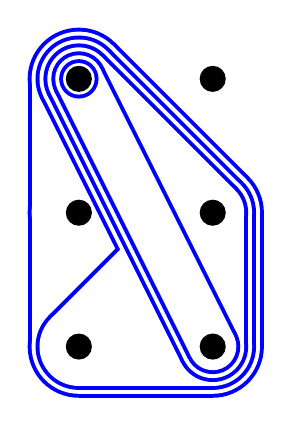
\begin{tikzpicture}
\node[fill] (1) at (0.0, 0.0) [circle] {};
\node[fill] (2) at (1.7, 0.0) [circle] {};
\node[fill] (3) at (0.0, -1.7) [circle] {};
\node[fill] (4) at (1.7, -1.7) [circle] {};
\node[fill] (5) at (0.0, -3.4) [circle] {};
\node[fill] (6) at (1.7, -3.4) [circle] {};
%13456
\begin{scope}[on background layer]
\fill[\tubecolor] (1) circle (\n + 9*\thickness);
\fill[\tubecolor] (3) circle (\n + 9*\thickness);
\fill[\tubecolor] (4) circle (\n + 9*\thickness);
\fill[\tubecolor] (5) circle (\n + 9*\thickness);
\fill[\tubecolor] (6) circle (\n + 9*\thickness);
\draw[\tubecolor] [line width = 2*(\n + 9*\thickness)] (1.center) -- (3.center);
\draw[\tubecolor] [line width = 2*(\n + 9*\thickness)] (1.center) -- (4.center);
\draw[\tubecolor] [line width = 2*(\n + 9*\thickness)] (1.center) -- (6.center);
\draw[\tubecolor] [line width = 2*(\n + 9*\thickness)] (3.center) -- (4.center);
\draw[\tubecolor] [line width = 2*(\n + 9*\thickness)] (3.center) -- (5.center);
\draw[\tubecolor] [line width = 2*(\n + 9*\thickness)] (3.center) -- (6.center);
\draw[\tubecolor] [line width = 2*(\n + 9*\thickness)] (4.center) -- (5.center);
\draw[\tubecolor] [line width = 2*(\n + 9*\thickness)] (4.center) -- (6.center);
\draw[\tubecolor] [line width = 2*(\n + 9*\thickness)] (5.center) -- (6.center);
\draw[white] [line width = 2*(\n + 8*\thickness)] (1.center) -- (3.center);
\draw[white] [line width = 2*(\n + 8*\thickness)] (1.center) -- (4.center);
\draw[white] [line width = 2*(\n + 8*\thickness)] (1.center) -- (6.center);
\draw[white] [line width = 2*(\n + 8*\thickness)] (3.center) -- (4.center);
\draw[white] [line width = 2*(\n + 8*\thickness)] (3.center) -- (5.center);
\draw[white] [line width = 2*(\n + 8*\thickness)] (3.center) -- (6.center);
\draw[white] [line width = 2*(\n + 8*\thickness)] (4.center) -- (5.center);
\draw[white] [line width = 2*(\n + 8*\thickness)] (4.center) -- (6.center);
\draw[white] [line width = 2*(\n + 8*\thickness)] (5.center) -- (6.center);
\fill[white] (1.center) -- (3.center) -- (4.center) -- (1.center);
\fill[white] (1.center) -- (3.center) -- (6.center) -- (1.center);
\fill[white] (4.center) -- (6.center) -- (1.center) -- (4.center);
\fill[white] (3.center) -- (5.center) -- (4.center) -- (3.center);
\fill[white] (4.center) -- (6.center) -- (3.center) -- (4.center);
\fill[white] (3.center) -- (5.center) -- (6.center) -- (3.center);
\fill[white] (4.center) -- (6.center) -- (5.center) -- (4.center);
\fill[white] (1) circle (\n + 8*\thickness);
\fill[white] (3) circle (\n + 8*\thickness);
\fill[white] (4) circle (\n + 8*\thickness);
\fill[white] (5) circle (\n + 8*\thickness);
\fill[white] (6) circle (\n + 8*\thickness);
\end{scope}
%1456
\begin{scope}[on background layer]
\fill[\tubecolor] (1) circle (\n + 7*\thickness);
\fill[\tubecolor] (4) circle (\n + 7*\thickness);
\fill[\tubecolor] (5) circle (\n + 7*\thickness);
\fill[\tubecolor] (6) circle (\n + 7*\thickness);
\draw[\tubecolor] [line width = 2*(\n + 7*\thickness)] (1.center) -- (4.center);
\draw[\tubecolor] [line width = 2*(\n + 7*\thickness)] (1.center) -- (6.center);
\draw[\tubecolor] [line width = 2*(\n + 7*\thickness)] (4.center) -- (5.center);
\draw[\tubecolor] [line width = 2*(\n + 7*\thickness)] (4.center) -- (6.center);
\draw[\tubecolor] [line width = 2*(\n + 7*\thickness)] (5.center) -- (6.center);
\draw[white] [line width = 2*(\n + 6*\thickness)] (1.center) -- (4.center);
\draw[white] [line width = 2*(\n + 6*\thickness)] (1.center) -- (6.center);
\draw[white] [line width = 2*(\n + 6*\thickness)] (4.center) -- (5.center);
\draw[white] [line width = 2*(\n + 6*\thickness)] (4.center) -- (6.center);
\draw[white] [line width = 2*(\n + 6*\thickness)] (5.center) -- (6.center);
\fill[white] (4.center) -- (6.center) -- (1.center) -- (4.center);
\fill[white] (4.center) -- (6.center) -- (5.center) -- (4.center);
\fill[white] (1) circle (\n + 6*\thickness);
\fill[white] (4) circle (\n + 6*\thickness);
\fill[white] (5) circle (\n + 6*\thickness);
\fill[white] (6) circle (\n + 6*\thickness);
\end{scope}
%146
\begin{scope}[on background layer]
\fill[\tubecolor] (1) circle (\n + 5*\thickness);
\fill[\tubecolor] (4) circle (\n + 5*\thickness);
\fill[\tubecolor] (6) circle (\n + 5*\thickness);
\draw[\tubecolor] [line width = 2*(\n + 5*\thickness)] (1.center) -- (4.center);
\draw[\tubecolor] [line width = 2*(\n + 5*\thickness)] (1.center) -- (6.center);
\draw[\tubecolor] [line width = 2*(\n + 5*\thickness)] (4.center) -- (6.center);
\draw[white] [line width = 2*(\n + 4*\thickness)] (1.center) -- (4.center);
\draw[white] [line width = 2*(\n + 4*\thickness)] (1.center) -- (6.center);
\draw[white] [line width = 2*(\n + 4*\thickness)] (4.center) -- (6.center);
\fill[white] (4.center) -- (6.center) -- (1.center) -- (4.center);
\fill[white] (1) circle (\n + 4*\thickness);
\fill[white] (4) circle (\n + 4*\thickness);
\fill[white] (6) circle (\n + 4*\thickness);
\end{scope}
%16
\begin{scope}[on background layer]
\fill[\tubecolor] (1) circle (\n + 3*\thickness);
\fill[\tubecolor] (6) circle (\n + 3*\thickness);
\draw[\tubecolor] [line width = 2*(\n + 3*\thickness)] (1.center) -- (6.center);
\draw[white] [line width = 2*(\n + 2*\thickness)] (1.center) -- (6.center);
\fill[white] (1) circle (\n + 2*\thickness);
\fill[white] (6) circle (\n + 2*\thickness);
\end{scope}
%1
\begin{scope}[on background layer]
\fill[\tubecolor] (1) circle (\n + 1*\thickness);
\fill[white] (1) circle (\n + 0*\thickness);
\end{scope}
\end{tikzpicture}
%165432
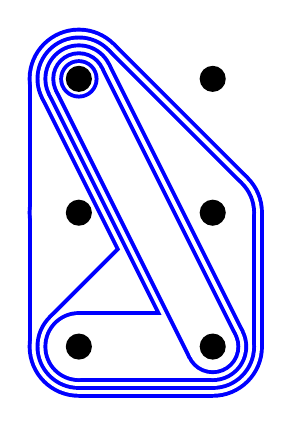
\begin{tikzpicture}
\node[fill] (1) at (0.0, 0.0) [circle] {};
\node[fill] (2) at (1.7, 0.0) [circle] {};
\node[fill] (3) at (0.0, -1.7) [circle] {};
\node[fill] (4) at (1.7, -1.7) [circle] {};
\node[fill] (5) at (0.0, -3.4) [circle] {};
\node[fill] (6) at (1.7, -3.4) [circle] {};
%13456
\begin{scope}[on background layer]
\fill[\tubecolor] (1) circle (\n + 9*\thickness);
\fill[\tubecolor] (3) circle (\n + 9*\thickness);
\fill[\tubecolor] (4) circle (\n + 9*\thickness);
\fill[\tubecolor] (5) circle (\n + 9*\thickness);
\fill[\tubecolor] (6) circle (\n + 9*\thickness);
\draw[\tubecolor] [line width = 2*(\n + 9*\thickness)] (1.center) -- (3.center);
\draw[\tubecolor] [line width = 2*(\n + 9*\thickness)] (1.center) -- (4.center);
\draw[\tubecolor] [line width = 2*(\n + 9*\thickness)] (1.center) -- (6.center);
\draw[\tubecolor] [line width = 2*(\n + 9*\thickness)] (3.center) -- (4.center);
\draw[\tubecolor] [line width = 2*(\n + 9*\thickness)] (3.center) -- (5.center);
\draw[\tubecolor] [line width = 2*(\n + 9*\thickness)] (3.center) -- (6.center);
\draw[\tubecolor] [line width = 2*(\n + 9*\thickness)] (4.center) -- (5.center);
\draw[\tubecolor] [line width = 2*(\n + 9*\thickness)] (4.center) -- (6.center);
\draw[\tubecolor] [line width = 2*(\n + 9*\thickness)] (5.center) -- (6.center);
\draw[white] [line width = 2*(\n + 8*\thickness)] (1.center) -- (3.center);
\draw[white] [line width = 2*(\n + 8*\thickness)] (1.center) -- (4.center);
\draw[white] [line width = 2*(\n + 8*\thickness)] (1.center) -- (6.center);
\draw[white] [line width = 2*(\n + 8*\thickness)] (3.center) -- (4.center);
\draw[white] [line width = 2*(\n + 8*\thickness)] (3.center) -- (5.center);
\draw[white] [line width = 2*(\n + 8*\thickness)] (3.center) -- (6.center);
\draw[white] [line width = 2*(\n + 8*\thickness)] (4.center) -- (5.center);
\draw[white] [line width = 2*(\n + 8*\thickness)] (4.center) -- (6.center);
\draw[white] [line width = 2*(\n + 8*\thickness)] (5.center) -- (6.center);
\fill[white] (1.center) -- (3.center) -- (4.center) -- (1.center);
\fill[white] (1.center) -- (3.center) -- (6.center) -- (1.center);
\fill[white] (4.center) -- (6.center) -- (1.center) -- (4.center);
\fill[white] (3.center) -- (5.center) -- (4.center) -- (3.center);
\fill[white] (4.center) -- (6.center) -- (3.center) -- (4.center);
\fill[white] (3.center) -- (5.center) -- (6.center) -- (3.center);
\fill[white] (4.center) -- (6.center) -- (5.center) -- (4.center);
\fill[white] (1) circle (\n + 8*\thickness);
\fill[white] (3) circle (\n + 8*\thickness);
\fill[white] (4) circle (\n + 8*\thickness);
\fill[white] (5) circle (\n + 8*\thickness);
\fill[white] (6) circle (\n + 8*\thickness);
\end{scope}
%1456
\begin{scope}[on background layer]
\fill[\tubecolor] (1) circle (\n + 7*\thickness);
\fill[\tubecolor] (4) circle (\n + 7*\thickness);
\fill[\tubecolor] (5) circle (\n + 7*\thickness);
\fill[\tubecolor] (6) circle (\n + 7*\thickness);
\draw[\tubecolor] [line width = 2*(\n + 7*\thickness)] (1.center) -- (4.center);
\draw[\tubecolor] [line width = 2*(\n + 7*\thickness)] (1.center) -- (6.center);
\draw[\tubecolor] [line width = 2*(\n + 7*\thickness)] (4.center) -- (5.center);
\draw[\tubecolor] [line width = 2*(\n + 7*\thickness)] (4.center) -- (6.center);
\draw[\tubecolor] [line width = 2*(\n + 7*\thickness)] (5.center) -- (6.center);
\draw[white] [line width = 2*(\n + 6*\thickness)] (1.center) -- (4.center);
\draw[white] [line width = 2*(\n + 6*\thickness)] (1.center) -- (6.center);
\draw[white] [line width = 2*(\n + 6*\thickness)] (4.center) -- (5.center);
\draw[white] [line width = 2*(\n + 6*\thickness)] (4.center) -- (6.center);
\draw[white] [line width = 2*(\n + 6*\thickness)] (5.center) -- (6.center);
\fill[white] (4.center) -- (6.center) -- (1.center) -- (4.center);
\fill[white] (4.center) -- (6.center) -- (5.center) -- (4.center);
\fill[white] (1) circle (\n + 6*\thickness);
\fill[white] (4) circle (\n + 6*\thickness);
\fill[white] (5) circle (\n + 6*\thickness);
\fill[white] (6) circle (\n + 6*\thickness);
\end{scope}
%156
\begin{scope}[on background layer]
\fill[\tubecolor] (1) circle (\n + 5*\thickness);
\fill[\tubecolor] (5) circle (\n + 5*\thickness);
\fill[\tubecolor] (6) circle (\n + 5*\thickness);
\draw[\tubecolor] [line width = 2*(\n + 5*\thickness)] (1.center) -- (6.center);
\draw[\tubecolor] [line width = 2*(\n + 5*\thickness)] (5.center) -- (6.center);
\draw[white] [line width = 2*(\n + 4*\thickness)] (1.center) -- (6.center);
\draw[white] [line width = 2*(\n + 4*\thickness)] (5.center) -- (6.center);
\fill[white] (1) circle (\n + 4*\thickness);
\fill[white] (5) circle (\n + 4*\thickness);
\fill[white] (6) circle (\n + 4*\thickness);
\end{scope}
%16
\begin{scope}[on background layer]
\fill[\tubecolor] (1) circle (\n + 3*\thickness);
\fill[\tubecolor] (6) circle (\n + 3*\thickness);
\draw[\tubecolor] [line width = 2*(\n + 3*\thickness)] (1.center) -- (6.center);
\draw[white] [line width = 2*(\n + 2*\thickness)] (1.center) -- (6.center);
\fill[white] (1) circle (\n + 2*\thickness);
\fill[white] (6) circle (\n + 2*\thickness);
\end{scope}
%1
\begin{scope}[on background layer]
\fill[\tubecolor] (1) circle (\n + 1*\thickness);
\fill[white] (1) circle (\n + 0*\thickness);
\end{scope}
\end{tikzpicture}
%165342
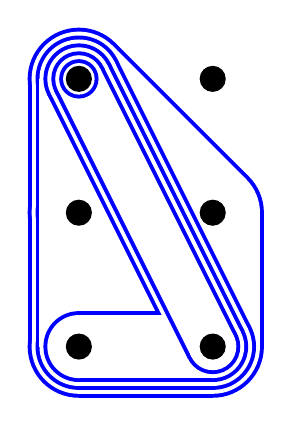
\begin{tikzpicture}
\node[fill] (1) at (0.0, 0.0) [circle] {};
\node[fill] (2) at (1.7, 0.0) [circle] {};
\node[fill] (3) at (0.0, -1.7) [circle] {};
\node[fill] (4) at (1.7, -1.7) [circle] {};
\node[fill] (5) at (0.0, -3.4) [circle] {};
\node[fill] (6) at (1.7, -3.4) [circle] {};
%13456
\begin{scope}[on background layer]
\fill[\tubecolor] (1) circle (\n + 9*\thickness);
\fill[\tubecolor] (3) circle (\n + 9*\thickness);
\fill[\tubecolor] (4) circle (\n + 9*\thickness);
\fill[\tubecolor] (5) circle (\n + 9*\thickness);
\fill[\tubecolor] (6) circle (\n + 9*\thickness);
\draw[\tubecolor] [line width = 2*(\n + 9*\thickness)] (1.center) -- (3.center);
\draw[\tubecolor] [line width = 2*(\n + 9*\thickness)] (1.center) -- (4.center);
\draw[\tubecolor] [line width = 2*(\n + 9*\thickness)] (1.center) -- (6.center);
\draw[\tubecolor] [line width = 2*(\n + 9*\thickness)] (3.center) -- (4.center);
\draw[\tubecolor] [line width = 2*(\n + 9*\thickness)] (3.center) -- (5.center);
\draw[\tubecolor] [line width = 2*(\n + 9*\thickness)] (3.center) -- (6.center);
\draw[\tubecolor] [line width = 2*(\n + 9*\thickness)] (4.center) -- (5.center);
\draw[\tubecolor] [line width = 2*(\n + 9*\thickness)] (4.center) -- (6.center);
\draw[\tubecolor] [line width = 2*(\n + 9*\thickness)] (5.center) -- (6.center);
\draw[white] [line width = 2*(\n + 8*\thickness)] (1.center) -- (3.center);
\draw[white] [line width = 2*(\n + 8*\thickness)] (1.center) -- (4.center);
\draw[white] [line width = 2*(\n + 8*\thickness)] (1.center) -- (6.center);
\draw[white] [line width = 2*(\n + 8*\thickness)] (3.center) -- (4.center);
\draw[white] [line width = 2*(\n + 8*\thickness)] (3.center) -- (5.center);
\draw[white] [line width = 2*(\n + 8*\thickness)] (3.center) -- (6.center);
\draw[white] [line width = 2*(\n + 8*\thickness)] (4.center) -- (5.center);
\draw[white] [line width = 2*(\n + 8*\thickness)] (4.center) -- (6.center);
\draw[white] [line width = 2*(\n + 8*\thickness)] (5.center) -- (6.center);
\fill[white] (1.center) -- (3.center) -- (4.center) -- (1.center);
\fill[white] (1.center) -- (3.center) -- (6.center) -- (1.center);
\fill[white] (4.center) -- (6.center) -- (1.center) -- (4.center);
\fill[white] (3.center) -- (5.center) -- (4.center) -- (3.center);
\fill[white] (4.center) -- (6.center) -- (3.center) -- (4.center);
\fill[white] (3.center) -- (5.center) -- (6.center) -- (3.center);
\fill[white] (4.center) -- (6.center) -- (5.center) -- (4.center);
\fill[white] (1) circle (\n + 8*\thickness);
\fill[white] (3) circle (\n + 8*\thickness);
\fill[white] (4) circle (\n + 8*\thickness);
\fill[white] (5) circle (\n + 8*\thickness);
\fill[white] (6) circle (\n + 8*\thickness);
\end{scope}
%1356
\begin{scope}[on background layer]
\fill[\tubecolor] (1) circle (\n + 7*\thickness);
\fill[\tubecolor] (3) circle (\n + 7*\thickness);
\fill[\tubecolor] (5) circle (\n + 7*\thickness);
\fill[\tubecolor] (6) circle (\n + 7*\thickness);
\draw[\tubecolor] [line width = 2*(\n + 7*\thickness)] (1.center) -- (3.center);
\draw[\tubecolor] [line width = 2*(\n + 7*\thickness)] (1.center) -- (6.center);
\draw[\tubecolor] [line width = 2*(\n + 7*\thickness)] (3.center) -- (5.center);
\draw[\tubecolor] [line width = 2*(\n + 7*\thickness)] (3.center) -- (6.center);
\draw[\tubecolor] [line width = 2*(\n + 7*\thickness)] (5.center) -- (6.center);
\draw[white] [line width = 2*(\n + 6*\thickness)] (1.center) -- (3.center);
\draw[white] [line width = 2*(\n + 6*\thickness)] (1.center) -- (6.center);
\draw[white] [line width = 2*(\n + 6*\thickness)] (3.center) -- (5.center);
\draw[white] [line width = 2*(\n + 6*\thickness)] (3.center) -- (6.center);
\draw[white] [line width = 2*(\n + 6*\thickness)] (5.center) -- (6.center);
\fill[white] (1.center) -- (3.center) -- (6.center) -- (1.center);
\fill[white] (3.center) -- (5.center) -- (6.center) -- (3.center);
\fill[white] (1) circle (\n + 6*\thickness);
\fill[white] (3) circle (\n + 6*\thickness);
\fill[white] (5) circle (\n + 6*\thickness);
\fill[white] (6) circle (\n + 6*\thickness);
\end{scope}
%156
\begin{scope}[on background layer]
\fill[\tubecolor] (1) circle (\n + 5*\thickness);
\fill[\tubecolor] (5) circle (\n + 5*\thickness);
\fill[\tubecolor] (6) circle (\n + 5*\thickness);
\draw[\tubecolor] [line width = 2*(\n + 5*\thickness)] (1.center) -- (6.center);
\draw[\tubecolor] [line width = 2*(\n + 5*\thickness)] (5.center) -- (6.center);
\draw[white] [line width = 2*(\n + 4*\thickness)] (1.center) -- (6.center);
\draw[white] [line width = 2*(\n + 4*\thickness)] (5.center) -- (6.center);
\fill[white] (1) circle (\n + 4*\thickness);
\fill[white] (5) circle (\n + 4*\thickness);
\fill[white] (6) circle (\n + 4*\thickness);
\end{scope}
%16
\begin{scope}[on background layer]
\fill[\tubecolor] (1) circle (\n + 3*\thickness);
\fill[\tubecolor] (6) circle (\n + 3*\thickness);
\draw[\tubecolor] [line width = 2*(\n + 3*\thickness)] (1.center) -- (6.center);
\draw[white] [line width = 2*(\n + 2*\thickness)] (1.center) -- (6.center);
\fill[white] (1) circle (\n + 2*\thickness);
\fill[white] (6) circle (\n + 2*\thickness);
\end{scope}
%1
\begin{scope}[on background layer]
\fill[\tubecolor] (1) circle (\n + 1*\thickness);
\fill[white] (1) circle (\n + 0*\thickness);
\end{scope}
\end{tikzpicture}
%165324
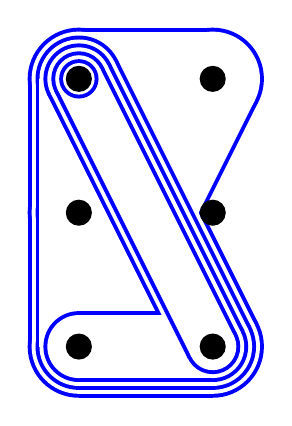
\begin{tikzpicture}
\node[fill] (1) at (0.0, 0.0) [circle] {};
\node[fill] (2) at (1.7, 0.0) [circle] {};
\node[fill] (3) at (0.0, -1.7) [circle] {};
\node[fill] (4) at (1.7, -1.7) [circle] {};
\node[fill] (5) at (0.0, -3.4) [circle] {};
\node[fill] (6) at (1.7, -3.4) [circle] {};
%12356
\begin{scope}[on background layer]
\fill[\tubecolor] (1) circle (\n + 9*\thickness);
\fill[\tubecolor] (2) circle (\n + 9*\thickness);
\fill[\tubecolor] (3) circle (\n + 9*\thickness);
\fill[\tubecolor] (5) circle (\n + 9*\thickness);
\fill[\tubecolor] (6) circle (\n + 9*\thickness);
\draw[\tubecolor] [line width = 2*(\n + 9*\thickness)] (1.center) -- (2.center);
\draw[\tubecolor] [line width = 2*(\n + 9*\thickness)] (1.center) -- (3.center);
\draw[\tubecolor] [line width = 2*(\n + 9*\thickness)] (1.center) -- (6.center);
\draw[\tubecolor] [line width = 2*(\n + 9*\thickness)] (2.center) -- (3.center);
\draw[\tubecolor] [line width = 2*(\n + 9*\thickness)] (2.center) -- (5.center);
\draw[\tubecolor] [line width = 2*(\n + 9*\thickness)] (3.center) -- (5.center);
\draw[\tubecolor] [line width = 2*(\n + 9*\thickness)] (3.center) -- (6.center);
\draw[\tubecolor] [line width = 2*(\n + 9*\thickness)] (5.center) -- (6.center);
\draw[white] [line width = 2*(\n + 8*\thickness)] (1.center) -- (2.center);
\draw[white] [line width = 2*(\n + 8*\thickness)] (1.center) -- (3.center);
\draw[white] [line width = 2*(\n + 8*\thickness)] (1.center) -- (6.center);
\draw[white] [line width = 2*(\n + 8*\thickness)] (2.center) -- (3.center);
\draw[white] [line width = 2*(\n + 8*\thickness)] (2.center) -- (5.center);
\draw[white] [line width = 2*(\n + 8*\thickness)] (3.center) -- (5.center);
\draw[white] [line width = 2*(\n + 8*\thickness)] (3.center) -- (6.center);
\draw[white] [line width = 2*(\n + 8*\thickness)] (5.center) -- (6.center);
\fill[white] (1.center) -- (3.center) -- (2.center) -- (1.center);
\fill[white] (1.center) -- (3.center) -- (6.center) -- (1.center);
\fill[white] (3.center) -- (5.center) -- (2.center) -- (3.center);
\fill[white] (3.center) -- (5.center) -- (6.center) -- (3.center);
\fill[white] (1) circle (\n + 8*\thickness);
\fill[white] (2) circle (\n + 8*\thickness);
\fill[white] (3) circle (\n + 8*\thickness);
\fill[white] (5) circle (\n + 8*\thickness);
\fill[white] (6) circle (\n + 8*\thickness);
\end{scope}
%1356
\begin{scope}[on background layer]
\fill[\tubecolor] (1) circle (\n + 7*\thickness);
\fill[\tubecolor] (3) circle (\n + 7*\thickness);
\fill[\tubecolor] (5) circle (\n + 7*\thickness);
\fill[\tubecolor] (6) circle (\n + 7*\thickness);
\draw[\tubecolor] [line width = 2*(\n + 7*\thickness)] (1.center) -- (3.center);
\draw[\tubecolor] [line width = 2*(\n + 7*\thickness)] (1.center) -- (6.center);
\draw[\tubecolor] [line width = 2*(\n + 7*\thickness)] (3.center) -- (5.center);
\draw[\tubecolor] [line width = 2*(\n + 7*\thickness)] (3.center) -- (6.center);
\draw[\tubecolor] [line width = 2*(\n + 7*\thickness)] (5.center) -- (6.center);
\draw[white] [line width = 2*(\n + 6*\thickness)] (1.center) -- (3.center);
\draw[white] [line width = 2*(\n + 6*\thickness)] (1.center) -- (6.center);
\draw[white] [line width = 2*(\n + 6*\thickness)] (3.center) -- (5.center);
\draw[white] [line width = 2*(\n + 6*\thickness)] (3.center) -- (6.center);
\draw[white] [line width = 2*(\n + 6*\thickness)] (5.center) -- (6.center);
\fill[white] (1.center) -- (3.center) -- (6.center) -- (1.center);
\fill[white] (3.center) -- (5.center) -- (6.center) -- (3.center);
\fill[white] (1) circle (\n + 6*\thickness);
\fill[white] (3) circle (\n + 6*\thickness);
\fill[white] (5) circle (\n + 6*\thickness);
\fill[white] (6) circle (\n + 6*\thickness);
\end{scope}
%156
\begin{scope}[on background layer]
\fill[\tubecolor] (1) circle (\n + 5*\thickness);
\fill[\tubecolor] (5) circle (\n + 5*\thickness);
\fill[\tubecolor] (6) circle (\n + 5*\thickness);
\draw[\tubecolor] [line width = 2*(\n + 5*\thickness)] (1.center) -- (6.center);
\draw[\tubecolor] [line width = 2*(\n + 5*\thickness)] (5.center) -- (6.center);
\draw[white] [line width = 2*(\n + 4*\thickness)] (1.center) -- (6.center);
\draw[white] [line width = 2*(\n + 4*\thickness)] (5.center) -- (6.center);
\fill[white] (1) circle (\n + 4*\thickness);
\fill[white] (5) circle (\n + 4*\thickness);
\fill[white] (6) circle (\n + 4*\thickness);
\end{scope}
%16
\begin{scope}[on background layer]
\fill[\tubecolor] (1) circle (\n + 3*\thickness);
\fill[\tubecolor] (6) circle (\n + 3*\thickness);
\draw[\tubecolor] [line width = 2*(\n + 3*\thickness)] (1.center) -- (6.center);
\draw[white] [line width = 2*(\n + 2*\thickness)] (1.center) -- (6.center);
\fill[white] (1) circle (\n + 2*\thickness);
\fill[white] (6) circle (\n + 2*\thickness);
\end{scope}
%1
\begin{scope}[on background layer]
\fill[\tubecolor] (1) circle (\n + 1*\thickness);
\fill[white] (1) circle (\n + 0*\thickness);
\end{scope}
\end{tikzpicture}
%165234
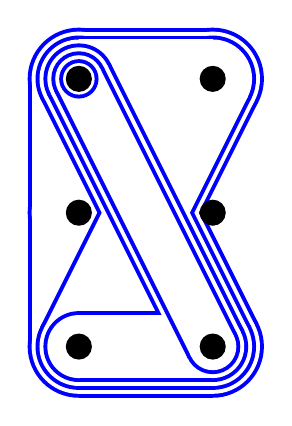
\begin{tikzpicture}
\node[fill] (1) at (0.0, 0.0) [circle] {};
\node[fill] (2) at (1.7, 0.0) [circle] {};
\node[fill] (3) at (0.0, -1.7) [circle] {};
\node[fill] (4) at (1.7, -1.7) [circle] {};
\node[fill] (5) at (0.0, -3.4) [circle] {};
\node[fill] (6) at (1.7, -3.4) [circle] {};
%12356
\begin{scope}[on background layer]
\fill[\tubecolor] (1) circle (\n + 9*\thickness);
\fill[\tubecolor] (2) circle (\n + 9*\thickness);
\fill[\tubecolor] (3) circle (\n + 9*\thickness);
\fill[\tubecolor] (5) circle (\n + 9*\thickness);
\fill[\tubecolor] (6) circle (\n + 9*\thickness);
\draw[\tubecolor] [line width = 2*(\n + 9*\thickness)] (1.center) -- (2.center);
\draw[\tubecolor] [line width = 2*(\n + 9*\thickness)] (1.center) -- (3.center);
\draw[\tubecolor] [line width = 2*(\n + 9*\thickness)] (1.center) -- (6.center);
\draw[\tubecolor] [line width = 2*(\n + 9*\thickness)] (2.center) -- (3.center);
\draw[\tubecolor] [line width = 2*(\n + 9*\thickness)] (2.center) -- (5.center);
\draw[\tubecolor] [line width = 2*(\n + 9*\thickness)] (3.center) -- (5.center);
\draw[\tubecolor] [line width = 2*(\n + 9*\thickness)] (3.center) -- (6.center);
\draw[\tubecolor] [line width = 2*(\n + 9*\thickness)] (5.center) -- (6.center);
\draw[white] [line width = 2*(\n + 8*\thickness)] (1.center) -- (2.center);
\draw[white] [line width = 2*(\n + 8*\thickness)] (1.center) -- (3.center);
\draw[white] [line width = 2*(\n + 8*\thickness)] (1.center) -- (6.center);
\draw[white] [line width = 2*(\n + 8*\thickness)] (2.center) -- (3.center);
\draw[white] [line width = 2*(\n + 8*\thickness)] (2.center) -- (5.center);
\draw[white] [line width = 2*(\n + 8*\thickness)] (3.center) -- (5.center);
\draw[white] [line width = 2*(\n + 8*\thickness)] (3.center) -- (6.center);
\draw[white] [line width = 2*(\n + 8*\thickness)] (5.center) -- (6.center);
\fill[white] (1.center) -- (3.center) -- (2.center) -- (1.center);
\fill[white] (1.center) -- (3.center) -- (6.center) -- (1.center);
\fill[white] (3.center) -- (5.center) -- (2.center) -- (3.center);
\fill[white] (3.center) -- (5.center) -- (6.center) -- (3.center);
\fill[white] (1) circle (\n + 8*\thickness);
\fill[white] (2) circle (\n + 8*\thickness);
\fill[white] (3) circle (\n + 8*\thickness);
\fill[white] (5) circle (\n + 8*\thickness);
\fill[white] (6) circle (\n + 8*\thickness);
\end{scope}
%1256
\begin{scope}[on background layer]
\fill[\tubecolor] (1) circle (\n + 7*\thickness);
\fill[\tubecolor] (2) circle (\n + 7*\thickness);
\fill[\tubecolor] (5) circle (\n + 7*\thickness);
\fill[\tubecolor] (6) circle (\n + 7*\thickness);
\draw[\tubecolor] [line width = 2*(\n + 7*\thickness)] (1.center) -- (2.center);
\draw[\tubecolor] [line width = 2*(\n + 7*\thickness)] (2.center) -- (5.center);
\draw[\tubecolor] [line width = 2*(\n + 7*\thickness)] (5.center) -- (6.center);
\draw[\tubecolor] [line width = 2*(\n + 7*\thickness)] (6.center) -- (1.center);
\draw[white] [line width = 2*(\n + 6*\thickness)] (1.center) -- (2.center);
\draw[white] [line width = 2*(\n + 6*\thickness)] (2.center) -- (5.center);
\draw[white] [line width = 2*(\n + 6*\thickness)] (5.center) -- (6.center);
\draw[white] [line width = 2*(\n + 6*\thickness)] (6.center) -- (1.center);
\fill[white] (1.center) -- (2.center) -- (5.center) -- (6.center) -- (1.center);
\fill[white] (1) circle (\n + 6*\thickness);
\fill[white] (2) circle (\n + 6*\thickness);
\fill[white] (5) circle (\n + 6*\thickness);
\fill[white] (6) circle (\n + 6*\thickness);
\end{scope}
%156
\begin{scope}[on background layer]
\fill[\tubecolor] (1) circle (\n + 5*\thickness);
\fill[\tubecolor] (5) circle (\n + 5*\thickness);
\fill[\tubecolor] (6) circle (\n + 5*\thickness);
\draw[\tubecolor] [line width = 2*(\n + 5*\thickness)] (1.center) -- (6.center);
\draw[\tubecolor] [line width = 2*(\n + 5*\thickness)] (5.center) -- (6.center);
\draw[white] [line width = 2*(\n + 4*\thickness)] (1.center) -- (6.center);
\draw[white] [line width = 2*(\n + 4*\thickness)] (5.center) -- (6.center);
\fill[white] (1) circle (\n + 4*\thickness);
\fill[white] (5) circle (\n + 4*\thickness);
\fill[white] (6) circle (\n + 4*\thickness);
\end{scope}
%16
\begin{scope}[on background layer]
\fill[\tubecolor] (1) circle (\n + 3*\thickness);
\fill[\tubecolor] (6) circle (\n + 3*\thickness);
\draw[\tubecolor] [line width = 2*(\n + 3*\thickness)] (1.center) -- (6.center);
\draw[white] [line width = 2*(\n + 2*\thickness)] (1.center) -- (6.center);
\fill[white] (1) circle (\n + 2*\thickness);
\fill[white] (6) circle (\n + 2*\thickness);
\end{scope}
%1
\begin{scope}[on background layer]
\fill[\tubecolor] (1) circle (\n + 1*\thickness);
\fill[white] (1) circle (\n + 0*\thickness);
\end{scope}
\end{tikzpicture}


%165243
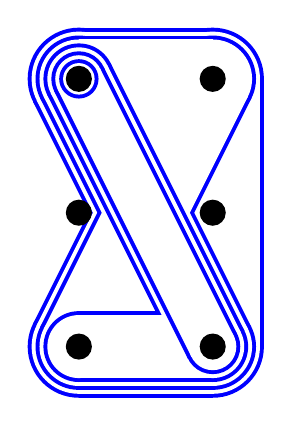
\begin{tikzpicture}
\node[fill] (1) at (0.0, 0.0) [circle] {};
\node[fill] (2) at (1.7, 0.0) [circle] {};
\node[fill] (3) at (0.0, -1.7) [circle] {};
\node[fill] (4) at (1.7, -1.7) [circle] {};
\node[fill] (5) at (0.0, -3.4) [circle] {};
\node[fill] (6) at (1.7, -3.4) [circle] {};
%12456
\begin{scope}[on background layer]
\fill[\tubecolor] (1) circle (\n + 9*\thickness);
\fill[\tubecolor] (2) circle (\n + 9*\thickness);
\fill[\tubecolor] (4) circle (\n + 9*\thickness);
\fill[\tubecolor] (5) circle (\n + 9*\thickness);
\fill[\tubecolor] (6) circle (\n + 9*\thickness);
\draw[\tubecolor] [line width = 2*(\n + 9*\thickness)] (1.center) -- (2.center);
\draw[\tubecolor] [line width = 2*(\n + 9*\thickness)] (1.center) -- (4.center);
\draw[\tubecolor] [line width = 2*(\n + 9*\thickness)] (1.center) -- (6.center);
\draw[\tubecolor] [line width = 2*(\n + 9*\thickness)] (2.center) -- (4.center);
\draw[\tubecolor] [line width = 2*(\n + 9*\thickness)] (2.center) -- (5.center);
\draw[\tubecolor] [line width = 2*(\n + 9*\thickness)] (4.center) -- (5.center);
\draw[\tubecolor] [line width = 2*(\n + 9*\thickness)] (4.center) -- (6.center);
\draw[\tubecolor] [line width = 2*(\n + 9*\thickness)] (5.center) -- (6.center);
\draw[white] [line width = 2*(\n + 8*\thickness)] (1.center) -- (2.center);
\draw[white] [line width = 2*(\n + 8*\thickness)] (1.center) -- (4.center);
\draw[white] [line width = 2*(\n + 8*\thickness)] (1.center) -- (6.center);
\draw[white] [line width = 2*(\n + 8*\thickness)] (2.center) -- (4.center);
\draw[white] [line width = 2*(\n + 8*\thickness)] (2.center) -- (5.center);
\draw[white] [line width = 2*(\n + 8*\thickness)] (4.center) -- (5.center);
\draw[white] [line width = 2*(\n + 8*\thickness)] (4.center) -- (6.center);
\draw[white] [line width = 2*(\n + 8*\thickness)] (5.center) -- (6.center);
\fill[white] (2.center) -- (4.center) -- (1.center) -- (2.center);
\fill[white] (4.center) -- (6.center) -- (1.center) -- (4.center);
\fill[white] (2.center) -- (4.center) -- (5.center) -- (2.center);
\fill[white] (4.center) -- (6.center) -- (5.center) -- (4.center);
\fill[white] (1) circle (\n + 8*\thickness);
\fill[white] (2) circle (\n + 8*\thickness);
\fill[white] (4) circle (\n + 8*\thickness);
\fill[white] (5) circle (\n + 8*\thickness);
\fill[white] (6) circle (\n + 8*\thickness);
\end{scope}
%1256
\begin{scope}[on background layer]
\fill[\tubecolor] (1) circle (\n + 7*\thickness);
\fill[\tubecolor] (2) circle (\n + 7*\thickness);
\fill[\tubecolor] (5) circle (\n + 7*\thickness);
\fill[\tubecolor] (6) circle (\n + 7*\thickness);
\draw[\tubecolor] [line width = 2*(\n + 7*\thickness)] (1.center) -- (2.center);
\draw[\tubecolor] [line width = 2*(\n + 7*\thickness)] (2.center) -- (5.center);
\draw[\tubecolor] [line width = 2*(\n + 7*\thickness)] (5.center) -- (6.center);
\draw[\tubecolor] [line width = 2*(\n + 7*\thickness)] (6.center) -- (1.center);
\draw[white] [line width = 2*(\n + 6*\thickness)] (1.center) -- (2.center);
\draw[white] [line width = 2*(\n + 6*\thickness)] (2.center) -- (5.center);
\draw[white] [line width = 2*(\n + 6*\thickness)] (5.center) -- (6.center);
\draw[white] [line width = 2*(\n + 6*\thickness)] (6.center) -- (1.center);
\fill[white] (1.center) -- (2.center) -- (5.center) -- (6.center) -- (1.center);
\fill[white] (1) circle (\n + 6*\thickness);
\fill[white] (2) circle (\n + 6*\thickness);
\fill[white] (5) circle (\n + 6*\thickness);
\fill[white] (6) circle (\n + 6*\thickness);
\end{scope}
%156
\begin{scope}[on background layer]
\fill[\tubecolor] (1) circle (\n + 5*\thickness);
\fill[\tubecolor] (5) circle (\n + 5*\thickness);
\fill[\tubecolor] (6) circle (\n + 5*\thickness);
\draw[\tubecolor] [line width = 2*(\n + 5*\thickness)] (1.center) -- (6.center);
\draw[\tubecolor] [line width = 2*(\n + 5*\thickness)] (5.center) -- (6.center);
\draw[white] [line width = 2*(\n + 4*\thickness)] (1.center) -- (6.center);
\draw[white] [line width = 2*(\n + 4*\thickness)] (5.center) -- (6.center);
\fill[white] (1) circle (\n + 4*\thickness);
\fill[white] (5) circle (\n + 4*\thickness);
\fill[white] (6) circle (\n + 4*\thickness);
\end{scope}
%16
\begin{scope}[on background layer]
\fill[\tubecolor] (1) circle (\n + 3*\thickness);
\fill[\tubecolor] (6) circle (\n + 3*\thickness);
\draw[\tubecolor] [line width = 2*(\n + 3*\thickness)] (1.center) -- (6.center);
\draw[white] [line width = 2*(\n + 2*\thickness)] (1.center) -- (6.center);
\fill[white] (1) circle (\n + 2*\thickness);
\fill[white] (6) circle (\n + 2*\thickness);
\end{scope}
%1
\begin{scope}[on background layer]
\fill[\tubecolor] (1) circle (\n + 1*\thickness);
\fill[white] (1) circle (\n + 0*\thickness);
\end{scope}
\end{tikzpicture}
%162543
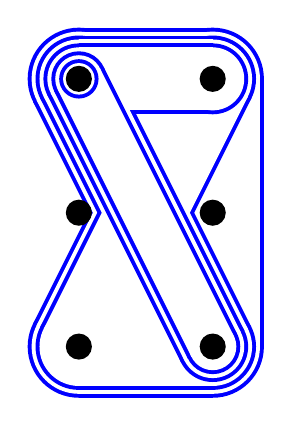
\begin{tikzpicture}
\node[fill] (1) at (0.0, 0.0) [circle] {};
\node[fill] (2) at (1.7, 0.0) [circle] {};
\node[fill] (3) at (0.0, -1.7) [circle] {};
\node[fill] (4) at (1.7, -1.7) [circle] {};
\node[fill] (5) at (0.0, -3.4) [circle] {};
\node[fill] (6) at (1.7, -3.4) [circle] {};
%12456
\begin{scope}[on background layer]
\fill[\tubecolor] (1) circle (\n + 9*\thickness);
\fill[\tubecolor] (2) circle (\n + 9*\thickness);
\fill[\tubecolor] (4) circle (\n + 9*\thickness);
\fill[\tubecolor] (5) circle (\n + 9*\thickness);
\fill[\tubecolor] (6) circle (\n + 9*\thickness);
\draw[\tubecolor] [line width = 2*(\n + 9*\thickness)] (1.center) -- (2.center);
\draw[\tubecolor] [line width = 2*(\n + 9*\thickness)] (1.center) -- (4.center);
\draw[\tubecolor] [line width = 2*(\n + 9*\thickness)] (1.center) -- (6.center);
\draw[\tubecolor] [line width = 2*(\n + 9*\thickness)] (2.center) -- (4.center);
\draw[\tubecolor] [line width = 2*(\n + 9*\thickness)] (2.center) -- (5.center);
\draw[\tubecolor] [line width = 2*(\n + 9*\thickness)] (4.center) -- (5.center);
\draw[\tubecolor] [line width = 2*(\n + 9*\thickness)] (4.center) -- (6.center);
\draw[\tubecolor] [line width = 2*(\n + 9*\thickness)] (5.center) -- (6.center);
\draw[white] [line width = 2*(\n + 8*\thickness)] (1.center) -- (2.center);
\draw[white] [line width = 2*(\n + 8*\thickness)] (1.center) -- (4.center);
\draw[white] [line width = 2*(\n + 8*\thickness)] (1.center) -- (6.center);
\draw[white] [line width = 2*(\n + 8*\thickness)] (2.center) -- (4.center);
\draw[white] [line width = 2*(\n + 8*\thickness)] (2.center) -- (5.center);
\draw[white] [line width = 2*(\n + 8*\thickness)] (4.center) -- (5.center);
\draw[white] [line width = 2*(\n + 8*\thickness)] (4.center) -- (6.center);
\draw[white] [line width = 2*(\n + 8*\thickness)] (5.center) -- (6.center);
\fill[white] (2.center) -- (4.center) -- (1.center) -- (2.center);
\fill[white] (4.center) -- (6.center) -- (1.center) -- (4.center);
\fill[white] (2.center) -- (4.center) -- (5.center) -- (2.center);
\fill[white] (4.center) -- (6.center) -- (5.center) -- (4.center);
\fill[white] (1) circle (\n + 8*\thickness);
\fill[white] (2) circle (\n + 8*\thickness);
\fill[white] (4) circle (\n + 8*\thickness);
\fill[white] (5) circle (\n + 8*\thickness);
\fill[white] (6) circle (\n + 8*\thickness);
\end{scope}
%1256
\begin{scope}[on background layer]
\fill[\tubecolor] (1) circle (\n + 7*\thickness);
\fill[\tubecolor] (2) circle (\n + 7*\thickness);
\fill[\tubecolor] (5) circle (\n + 7*\thickness);
\fill[\tubecolor] (6) circle (\n + 7*\thickness);
\draw[\tubecolor] [line width = 2*(\n + 7*\thickness)] (1.center) -- (2.center);
\draw[\tubecolor] [line width = 2*(\n + 7*\thickness)] (2.center) -- (5.center);
\draw[\tubecolor] [line width = 2*(\n + 7*\thickness)] (5.center) -- (6.center);
\draw[\tubecolor] [line width = 2*(\n + 7*\thickness)] (6.center) -- (1.center);
\draw[white] [line width = 2*(\n + 6*\thickness)] (1.center) -- (2.center);
\draw[white] [line width = 2*(\n + 6*\thickness)] (2.center) -- (5.center);
\draw[white] [line width = 2*(\n + 6*\thickness)] (5.center) -- (6.center);
\draw[white] [line width = 2*(\n + 6*\thickness)] (6.center) -- (1.center);
\fill[white] (1.center) -- (2.center) -- (5.center) -- (6.center) -- (1.center);
\fill[white] (1) circle (\n + 6*\thickness);
\fill[white] (2) circle (\n + 6*\thickness);
\fill[white] (5) circle (\n + 6*\thickness);
\fill[white] (6) circle (\n + 6*\thickness);
\end{scope}
%126
\begin{scope}[on background layer]
\fill[\tubecolor] (1) circle (\n + 5*\thickness);
\fill[\tubecolor] (2) circle (\n + 5*\thickness);
\fill[\tubecolor] (6) circle (\n + 5*\thickness);
\draw[\tubecolor] [line width = 2*(\n + 5*\thickness)] (1.center) -- (2.center);
\draw[\tubecolor] [line width = 2*(\n + 5*\thickness)] (1.center) -- (6.center);
\draw[white] [line width = 2*(\n + 4*\thickness)] (1.center) -- (2.center);
\draw[white] [line width = 2*(\n + 4*\thickness)] (1.center) -- (6.center);
\fill[white] (1) circle (\n + 4*\thickness);
\fill[white] (2) circle (\n + 4*\thickness);
\fill[white] (6) circle (\n + 4*\thickness);
\end{scope}
%16
\begin{scope}[on background layer]
\fill[\tubecolor] (1) circle (\n + 3*\thickness);
\fill[\tubecolor] (6) circle (\n + 3*\thickness);
\draw[\tubecolor] [line width = 2*(\n + 3*\thickness)] (1.center) -- (6.center);
\draw[white] [line width = 2*(\n + 2*\thickness)] (1.center) -- (6.center);
\fill[white] (1) circle (\n + 2*\thickness);
\fill[white] (6) circle (\n + 2*\thickness);
\end{scope}
%1
\begin{scope}[on background layer]
\fill[\tubecolor] (1) circle (\n + 1*\thickness);
\fill[white] (1) circle (\n + 0*\thickness);
\end{scope}
\end{tikzpicture}
%162453
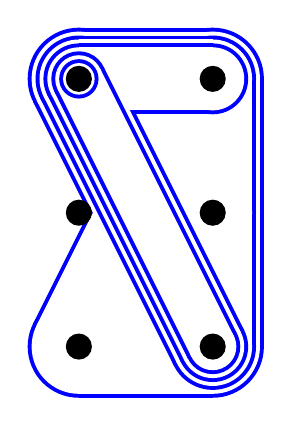
\begin{tikzpicture}
\node[fill] (1) at (0.0, 0.0) [circle] {};
\node[fill] (2) at (1.7, 0.0) [circle] {};
\node[fill] (3) at (0.0, -1.7) [circle] {};
\node[fill] (4) at (1.7, -1.7) [circle] {};
\node[fill] (5) at (0.0, -3.4) [circle] {};
\node[fill] (6) at (1.7, -3.4) [circle] {};
%12456
\begin{scope}[on background layer]
\fill[\tubecolor] (1) circle (\n + 9*\thickness);
\fill[\tubecolor] (2) circle (\n + 9*\thickness);
\fill[\tubecolor] (4) circle (\n + 9*\thickness);
\fill[\tubecolor] (5) circle (\n + 9*\thickness);
\fill[\tubecolor] (6) circle (\n + 9*\thickness);
\draw[\tubecolor] [line width = 2*(\n + 9*\thickness)] (1.center) -- (2.center);
\draw[\tubecolor] [line width = 2*(\n + 9*\thickness)] (1.center) -- (4.center);
\draw[\tubecolor] [line width = 2*(\n + 9*\thickness)] (1.center) -- (6.center);
\draw[\tubecolor] [line width = 2*(\n + 9*\thickness)] (2.center) -- (4.center);
\draw[\tubecolor] [line width = 2*(\n + 9*\thickness)] (2.center) -- (5.center);
\draw[\tubecolor] [line width = 2*(\n + 9*\thickness)] (4.center) -- (5.center);
\draw[\tubecolor] [line width = 2*(\n + 9*\thickness)] (4.center) -- (6.center);
\draw[\tubecolor] [line width = 2*(\n + 9*\thickness)] (5.center) -- (6.center);
\draw[white] [line width = 2*(\n + 8*\thickness)] (1.center) -- (2.center);
\draw[white] [line width = 2*(\n + 8*\thickness)] (1.center) -- (4.center);
\draw[white] [line width = 2*(\n + 8*\thickness)] (1.center) -- (6.center);
\draw[white] [line width = 2*(\n + 8*\thickness)] (2.center) -- (4.center);
\draw[white] [line width = 2*(\n + 8*\thickness)] (2.center) -- (5.center);
\draw[white] [line width = 2*(\n + 8*\thickness)] (4.center) -- (5.center);
\draw[white] [line width = 2*(\n + 8*\thickness)] (4.center) -- (6.center);
\draw[white] [line width = 2*(\n + 8*\thickness)] (5.center) -- (6.center);
\fill[white] (2.center) -- (4.center) -- (1.center) -- (2.center);
\fill[white] (4.center) -- (6.center) -- (1.center) -- (4.center);
\fill[white] (2.center) -- (4.center) -- (5.center) -- (2.center);
\fill[white] (4.center) -- (6.center) -- (5.center) -- (4.center);
\fill[white] (1) circle (\n + 8*\thickness);
\fill[white] (2) circle (\n + 8*\thickness);
\fill[white] (4) circle (\n + 8*\thickness);
\fill[white] (5) circle (\n + 8*\thickness);
\fill[white] (6) circle (\n + 8*\thickness);
\end{scope}
%1246
\begin{scope}[on background layer]
\fill[\tubecolor] (1) circle (\n + 7*\thickness);
\fill[\tubecolor] (2) circle (\n + 7*\thickness);
\fill[\tubecolor] (4) circle (\n + 7*\thickness);
\fill[\tubecolor] (6) circle (\n + 7*\thickness);
\draw[\tubecolor] [line width = 2*(\n + 7*\thickness)] (1.center) -- (2.center);
\draw[\tubecolor] [line width = 2*(\n + 7*\thickness)] (1.center) -- (4.center);
\draw[\tubecolor] [line width = 2*(\n + 7*\thickness)] (1.center) -- (6.center);
\draw[\tubecolor] [line width = 2*(\n + 7*\thickness)] (2.center) -- (4.center);
\draw[\tubecolor] [line width = 2*(\n + 7*\thickness)] (4.center) -- (6.center);
\draw[white] [line width = 2*(\n + 6*\thickness)] (1.center) -- (2.center);
\draw[white] [line width = 2*(\n + 6*\thickness)] (1.center) -- (4.center);
\draw[white] [line width = 2*(\n + 6*\thickness)] (1.center) -- (6.center);
\draw[white] [line width = 2*(\n + 6*\thickness)] (2.center) -- (4.center);
\draw[white] [line width = 2*(\n + 6*\thickness)] (4.center) -- (6.center);
\fill[white] (2.center) -- (4.center) -- (1.center) -- (2.center);
\fill[white] (4.center) -- (6.center) -- (1.center) -- (4.center);
\fill[white] (1) circle (\n + 6*\thickness);
\fill[white] (2) circle (\n + 6*\thickness);
\fill[white] (4) circle (\n + 6*\thickness);
\fill[white] (6) circle (\n + 6*\thickness);
\end{scope}
%126
\begin{scope}[on background layer]
\fill[\tubecolor] (1) circle (\n + 5*\thickness);
\fill[\tubecolor] (2) circle (\n + 5*\thickness);
\fill[\tubecolor] (6) circle (\n + 5*\thickness);
\draw[\tubecolor] [line width = 2*(\n + 5*\thickness)] (1.center) -- (2.center);
\draw[\tubecolor] [line width = 2*(\n + 5*\thickness)] (1.center) -- (6.center);
\draw[white] [line width = 2*(\n + 4*\thickness)] (1.center) -- (2.center);
\draw[white] [line width = 2*(\n + 4*\thickness)] (1.center) -- (6.center);
\fill[white] (1) circle (\n + 4*\thickness);
\fill[white] (2) circle (\n + 4*\thickness);
\fill[white] (6) circle (\n + 4*\thickness);
\end{scope}
%16
\begin{scope}[on background layer]
\fill[\tubecolor] (1) circle (\n + 3*\thickness);
\fill[\tubecolor] (6) circle (\n + 3*\thickness);
\draw[\tubecolor] [line width = 2*(\n + 3*\thickness)] (1.center) -- (6.center);
\draw[white] [line width = 2*(\n + 2*\thickness)] (1.center) -- (6.center);
\fill[white] (1) circle (\n + 2*\thickness);
\fill[white] (6) circle (\n + 2*\thickness);
\end{scope}
%1
\begin{scope}[on background layer]
\fill[\tubecolor] (1) circle (\n + 1*\thickness);
\fill[white] (1) circle (\n + 0*\thickness);
\end{scope}
\end{tikzpicture}
%162435
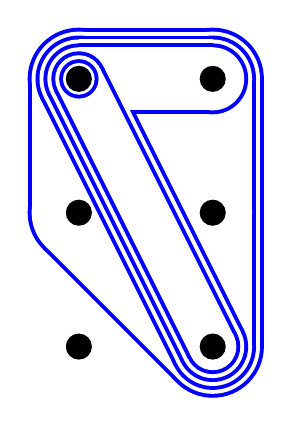
\begin{tikzpicture}
\node[fill] (1) at (0.0, 0.0) [circle] {};
\node[fill] (2) at (1.7, 0.0) [circle] {};
\node[fill] (3) at (0.0, -1.7) [circle] {};
\node[fill] (4) at (1.7, -1.7) [circle] {};
\node[fill] (5) at (0.0, -3.4) [circle] {};
\node[fill] (6) at (1.7, -3.4) [circle] {};
%12346
\begin{scope}[on background layer]
\fill[\tubecolor] (1) circle (\n + 9*\thickness);
\fill[\tubecolor] (2) circle (\n + 9*\thickness);
\fill[\tubecolor] (3) circle (\n + 9*\thickness);
\fill[\tubecolor] (4) circle (\n + 9*\thickness);
\fill[\tubecolor] (6) circle (\n + 9*\thickness);
\draw[\tubecolor] [line width = 2*(\n + 9*\thickness)] (1.center) -- (2.center);
\draw[\tubecolor] [line width = 2*(\n + 9*\thickness)] (1.center) -- (3.center);
\draw[\tubecolor] [line width = 2*(\n + 9*\thickness)] (1.center) -- (4.center);
\draw[\tubecolor] [line width = 2*(\n + 9*\thickness)] (1.center) -- (6.center);
\draw[\tubecolor] [line width = 2*(\n + 9*\thickness)] (2.center) -- (3.center);
\draw[\tubecolor] [line width = 2*(\n + 9*\thickness)] (2.center) -- (4.center);
\draw[\tubecolor] [line width = 2*(\n + 9*\thickness)] (3.center) -- (4.center);
\draw[\tubecolor] [line width = 2*(\n + 9*\thickness)] (3.center) -- (6.center);
\draw[\tubecolor] [line width = 2*(\n + 9*\thickness)] (4.center) -- (6.center);
\draw[white] [line width = 2*(\n + 8*\thickness)] (1.center) -- (2.center);
\draw[white] [line width = 2*(\n + 8*\thickness)] (1.center) -- (3.center);
\draw[white] [line width = 2*(\n + 8*\thickness)] (1.center) -- (4.center);
\draw[white] [line width = 2*(\n + 8*\thickness)] (1.center) -- (6.center);
\draw[white] [line width = 2*(\n + 8*\thickness)] (2.center) -- (3.center);
\draw[white] [line width = 2*(\n + 8*\thickness)] (2.center) -- (4.center);
\draw[white] [line width = 2*(\n + 8*\thickness)] (3.center) -- (4.center);
\draw[white] [line width = 2*(\n + 8*\thickness)] (3.center) -- (6.center);
\draw[white] [line width = 2*(\n + 8*\thickness)] (4.center) -- (6.center);
\fill[white] (1.center) -- (3.center) -- (2.center) -- (1.center);
\fill[white] (2.center) -- (4.center) -- (1.center) -- (2.center);
\fill[white] (1.center) -- (3.center) -- (4.center) -- (1.center);
\fill[white] (1.center) -- (3.center) -- (6.center) -- (1.center);
\fill[white] (4.center) -- (6.center) -- (1.center) -- (4.center);
\fill[white] (2.center) -- (4.center) -- (3.center) -- (2.center);
\fill[white] (4.center) -- (6.center) -- (3.center) -- (4.center);
\fill[white] (1) circle (\n + 8*\thickness);
\fill[white] (2) circle (\n + 8*\thickness);
\fill[white] (3) circle (\n + 8*\thickness);
\fill[white] (4) circle (\n + 8*\thickness);
\fill[white] (6) circle (\n + 8*\thickness);
\end{scope}
%1246
\begin{scope}[on background layer]
\fill[\tubecolor] (1) circle (\n + 7*\thickness);
\fill[\tubecolor] (2) circle (\n + 7*\thickness);
\fill[\tubecolor] (4) circle (\n + 7*\thickness);
\fill[\tubecolor] (6) circle (\n + 7*\thickness);
\draw[\tubecolor] [line width = 2*(\n + 7*\thickness)] (1.center) -- (2.center);
\draw[\tubecolor] [line width = 2*(\n + 7*\thickness)] (1.center) -- (4.center);
\draw[\tubecolor] [line width = 2*(\n + 7*\thickness)] (1.center) -- (6.center);
\draw[\tubecolor] [line width = 2*(\n + 7*\thickness)] (2.center) -- (4.center);
\draw[\tubecolor] [line width = 2*(\n + 7*\thickness)] (4.center) -- (6.center);
\draw[white] [line width = 2*(\n + 6*\thickness)] (1.center) -- (2.center);
\draw[white] [line width = 2*(\n + 6*\thickness)] (1.center) -- (4.center);
\draw[white] [line width = 2*(\n + 6*\thickness)] (1.center) -- (6.center);
\draw[white] [line width = 2*(\n + 6*\thickness)] (2.center) -- (4.center);
\draw[white] [line width = 2*(\n + 6*\thickness)] (4.center) -- (6.center);
\fill[white] (2.center) -- (4.center) -- (1.center) -- (2.center);
\fill[white] (4.center) -- (6.center) -- (1.center) -- (4.center);
\fill[white] (1) circle (\n + 6*\thickness);
\fill[white] (2) circle (\n + 6*\thickness);
\fill[white] (4) circle (\n + 6*\thickness);
\fill[white] (6) circle (\n + 6*\thickness);
\end{scope}
%126
\begin{scope}[on background layer]
\fill[\tubecolor] (1) circle (\n + 5*\thickness);
\fill[\tubecolor] (2) circle (\n + 5*\thickness);
\fill[\tubecolor] (6) circle (\n + 5*\thickness);
\draw[\tubecolor] [line width = 2*(\n + 5*\thickness)] (1.center) -- (2.center);
\draw[\tubecolor] [line width = 2*(\n + 5*\thickness)] (1.center) -- (6.center);
\draw[white] [line width = 2*(\n + 4*\thickness)] (1.center) -- (2.center);
\draw[white] [line width = 2*(\n + 4*\thickness)] (1.center) -- (6.center);
\fill[white] (1) circle (\n + 4*\thickness);
\fill[white] (2) circle (\n + 4*\thickness);
\fill[white] (6) circle (\n + 4*\thickness);
\end{scope}
%16
\begin{scope}[on background layer]
\fill[\tubecolor] (1) circle (\n + 3*\thickness);
\fill[\tubecolor] (6) circle (\n + 3*\thickness);
\draw[\tubecolor] [line width = 2*(\n + 3*\thickness)] (1.center) -- (6.center);
\draw[white] [line width = 2*(\n + 2*\thickness)] (1.center) -- (6.center);
\fill[white] (1) circle (\n + 2*\thickness);
\fill[white] (6) circle (\n + 2*\thickness);
\end{scope}
%1
\begin{scope}[on background layer]
\fill[\tubecolor] (1) circle (\n + 1*\thickness);
\fill[white] (1) circle (\n + 0*\thickness);
\end{scope}
\end{tikzpicture}
%162345
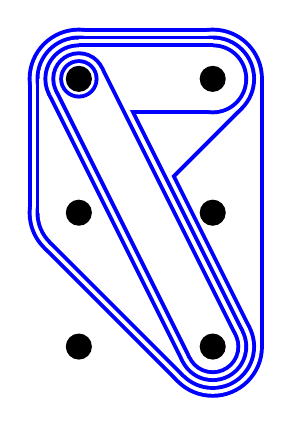
\begin{tikzpicture}
\node[fill] (1) at (0.0, 0.0) [circle] {};
\node[fill] (2) at (1.7, 0.0) [circle] {};
\node[fill] (3) at (0.0, -1.7) [circle] {};
\node[fill] (4) at (1.7, -1.7) [circle] {};
\node[fill] (5) at (0.0, -3.4) [circle] {};
\node[fill] (6) at (1.7, -3.4) [circle] {};
%12346
\begin{scope}[on background layer]
\fill[\tubecolor] (1) circle (\n + 9*\thickness);
\fill[\tubecolor] (2) circle (\n + 9*\thickness);
\fill[\tubecolor] (3) circle (\n + 9*\thickness);
\fill[\tubecolor] (4) circle (\n + 9*\thickness);
\fill[\tubecolor] (6) circle (\n + 9*\thickness);
\draw[\tubecolor] [line width = 2*(\n + 9*\thickness)] (1.center) -- (2.center);
\draw[\tubecolor] [line width = 2*(\n + 9*\thickness)] (1.center) -- (3.center);
\draw[\tubecolor] [line width = 2*(\n + 9*\thickness)] (1.center) -- (4.center);
\draw[\tubecolor] [line width = 2*(\n + 9*\thickness)] (1.center) -- (6.center);
\draw[\tubecolor] [line width = 2*(\n + 9*\thickness)] (2.center) -- (3.center);
\draw[\tubecolor] [line width = 2*(\n + 9*\thickness)] (2.center) -- (4.center);
\draw[\tubecolor] [line width = 2*(\n + 9*\thickness)] (3.center) -- (4.center);
\draw[\tubecolor] [line width = 2*(\n + 9*\thickness)] (3.center) -- (6.center);
\draw[\tubecolor] [line width = 2*(\n + 9*\thickness)] (4.center) -- (6.center);
\draw[white] [line width = 2*(\n + 8*\thickness)] (1.center) -- (2.center);
\draw[white] [line width = 2*(\n + 8*\thickness)] (1.center) -- (3.center);
\draw[white] [line width = 2*(\n + 8*\thickness)] (1.center) -- (4.center);
\draw[white] [line width = 2*(\n + 8*\thickness)] (1.center) -- (6.center);
\draw[white] [line width = 2*(\n + 8*\thickness)] (2.center) -- (3.center);
\draw[white] [line width = 2*(\n + 8*\thickness)] (2.center) -- (4.center);
\draw[white] [line width = 2*(\n + 8*\thickness)] (3.center) -- (4.center);
\draw[white] [line width = 2*(\n + 8*\thickness)] (3.center) -- (6.center);
\draw[white] [line width = 2*(\n + 8*\thickness)] (4.center) -- (6.center);
\fill[white] (1.center) -- (3.center) -- (2.center) -- (1.center);
\fill[white] (2.center) -- (4.center) -- (1.center) -- (2.center);
\fill[white] (1.center) -- (3.center) -- (4.center) -- (1.center);
\fill[white] (1.center) -- (3.center) -- (6.center) -- (1.center);
\fill[white] (4.center) -- (6.center) -- (1.center) -- (4.center);
\fill[white] (2.center) -- (4.center) -- (3.center) -- (2.center);
\fill[white] (4.center) -- (6.center) -- (3.center) -- (4.center);
\fill[white] (1) circle (\n + 8*\thickness);
\fill[white] (2) circle (\n + 8*\thickness);
\fill[white] (3) circle (\n + 8*\thickness);
\fill[white] (4) circle (\n + 8*\thickness);
\fill[white] (6) circle (\n + 8*\thickness);
\end{scope}
%1236
\begin{scope}[on background layer]
\fill[\tubecolor] (1) circle (\n + 7*\thickness);
\fill[\tubecolor] (2) circle (\n + 7*\thickness);
\fill[\tubecolor] (3) circle (\n + 7*\thickness);
\fill[\tubecolor] (6) circle (\n + 7*\thickness);
\draw[\tubecolor] [line width = 2*(\n + 7*\thickness)] (1.center) -- (2.center);
\draw[\tubecolor] [line width = 2*(\n + 7*\thickness)] (1.center) -- (3.center);
\draw[\tubecolor] [line width = 2*(\n + 7*\thickness)] (1.center) -- (6.center);
\draw[\tubecolor] [line width = 2*(\n + 7*\thickness)] (2.center) -- (3.center);
\draw[\tubecolor] [line width = 2*(\n + 7*\thickness)] (3.center) -- (6.center);
\draw[white] [line width = 2*(\n + 6*\thickness)] (1.center) -- (2.center);
\draw[white] [line width = 2*(\n + 6*\thickness)] (1.center) -- (3.center);
\draw[white] [line width = 2*(\n + 6*\thickness)] (1.center) -- (6.center);
\draw[white] [line width = 2*(\n + 6*\thickness)] (2.center) -- (3.center);
\draw[white] [line width = 2*(\n + 6*\thickness)] (3.center) -- (6.center);
\fill[white] (1.center) -- (3.center) -- (2.center) -- (1.center);
\fill[white] (1.center) -- (3.center) -- (6.center) -- (1.center);
\fill[white] (1) circle (\n + 6*\thickness);
\fill[white] (2) circle (\n + 6*\thickness);
\fill[white] (3) circle (\n + 6*\thickness);
\fill[white] (6) circle (\n + 6*\thickness);
\end{scope}
%126
\begin{scope}[on background layer]
\fill[\tubecolor] (1) circle (\n + 5*\thickness);
\fill[\tubecolor] (2) circle (\n + 5*\thickness);
\fill[\tubecolor] (6) circle (\n + 5*\thickness);
\draw[\tubecolor] [line width = 2*(\n + 5*\thickness)] (1.center) -- (2.center);
\draw[\tubecolor] [line width = 2*(\n + 5*\thickness)] (1.center) -- (6.center);
\draw[white] [line width = 2*(\n + 4*\thickness)] (1.center) -- (2.center);
\draw[white] [line width = 2*(\n + 4*\thickness)] (1.center) -- (6.center);
\fill[white] (1) circle (\n + 4*\thickness);
\fill[white] (2) circle (\n + 4*\thickness);
\fill[white] (6) circle (\n + 4*\thickness);
\end{scope}
%16
\begin{scope}[on background layer]
\fill[\tubecolor] (1) circle (\n + 3*\thickness);
\fill[\tubecolor] (6) circle (\n + 3*\thickness);
\draw[\tubecolor] [line width = 2*(\n + 3*\thickness)] (1.center) -- (6.center);
\draw[white] [line width = 2*(\n + 2*\thickness)] (1.center) -- (6.center);
\fill[white] (1) circle (\n + 2*\thickness);
\fill[white] (6) circle (\n + 2*\thickness);
\end{scope}
%1
\begin{scope}[on background layer]
\fill[\tubecolor] (1) circle (\n + 1*\thickness);
\fill[white] (1) circle (\n + 0*\thickness);
\end{scope}
\end{tikzpicture}
%163245
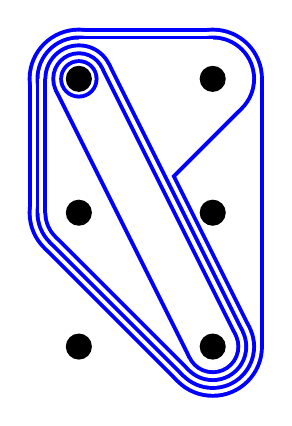
\begin{tikzpicture}
\node[fill] (1) at (0.0, 0.0) [circle] {};
\node[fill] (2) at (1.7, 0.0) [circle] {};
\node[fill] (3) at (0.0, -1.7) [circle] {};
\node[fill] (4) at (1.7, -1.7) [circle] {};
\node[fill] (5) at (0.0, -3.4) [circle] {};
\node[fill] (6) at (1.7, -3.4) [circle] {};
%12346
\begin{scope}[on background layer]
\fill[\tubecolor] (1) circle (\n + 9*\thickness);
\fill[\tubecolor] (2) circle (\n + 9*\thickness);
\fill[\tubecolor] (3) circle (\n + 9*\thickness);
\fill[\tubecolor] (4) circle (\n + 9*\thickness);
\fill[\tubecolor] (6) circle (\n + 9*\thickness);
\draw[\tubecolor] [line width = 2*(\n + 9*\thickness)] (1.center) -- (2.center);
\draw[\tubecolor] [line width = 2*(\n + 9*\thickness)] (1.center) -- (3.center);
\draw[\tubecolor] [line width = 2*(\n + 9*\thickness)] (1.center) -- (4.center);
\draw[\tubecolor] [line width = 2*(\n + 9*\thickness)] (1.center) -- (6.center);
\draw[\tubecolor] [line width = 2*(\n + 9*\thickness)] (2.center) -- (3.center);
\draw[\tubecolor] [line width = 2*(\n + 9*\thickness)] (2.center) -- (4.center);
\draw[\tubecolor] [line width = 2*(\n + 9*\thickness)] (3.center) -- (4.center);
\draw[\tubecolor] [line width = 2*(\n + 9*\thickness)] (3.center) -- (6.center);
\draw[\tubecolor] [line width = 2*(\n + 9*\thickness)] (4.center) -- (6.center);
\draw[white] [line width = 2*(\n + 8*\thickness)] (1.center) -- (2.center);
\draw[white] [line width = 2*(\n + 8*\thickness)] (1.center) -- (3.center);
\draw[white] [line width = 2*(\n + 8*\thickness)] (1.center) -- (4.center);
\draw[white] [line width = 2*(\n + 8*\thickness)] (1.center) -- (6.center);
\draw[white] [line width = 2*(\n + 8*\thickness)] (2.center) -- (3.center);
\draw[white] [line width = 2*(\n + 8*\thickness)] (2.center) -- (4.center);
\draw[white] [line width = 2*(\n + 8*\thickness)] (3.center) -- (4.center);
\draw[white] [line width = 2*(\n + 8*\thickness)] (3.center) -- (6.center);
\draw[white] [line width = 2*(\n + 8*\thickness)] (4.center) -- (6.center);
\fill[white] (1.center) -- (3.center) -- (2.center) -- (1.center);
\fill[white] (2.center) -- (4.center) -- (1.center) -- (2.center);
\fill[white] (1.center) -- (3.center) -- (4.center) -- (1.center);
\fill[white] (1.center) -- (3.center) -- (6.center) -- (1.center);
\fill[white] (4.center) -- (6.center) -- (1.center) -- (4.center);
\fill[white] (2.center) -- (4.center) -- (3.center) -- (2.center);
\fill[white] (4.center) -- (6.center) -- (3.center) -- (4.center);
\fill[white] (1) circle (\n + 8*\thickness);
\fill[white] (2) circle (\n + 8*\thickness);
\fill[white] (3) circle (\n + 8*\thickness);
\fill[white] (4) circle (\n + 8*\thickness);
\fill[white] (6) circle (\n + 8*\thickness);
\end{scope}
%1236
\begin{scope}[on background layer]
\fill[\tubecolor] (1) circle (\n + 7*\thickness);
\fill[\tubecolor] (2) circle (\n + 7*\thickness);
\fill[\tubecolor] (3) circle (\n + 7*\thickness);
\fill[\tubecolor] (6) circle (\n + 7*\thickness);
\draw[\tubecolor] [line width = 2*(\n + 7*\thickness)] (1.center) -- (2.center);
\draw[\tubecolor] [line width = 2*(\n + 7*\thickness)] (1.center) -- (3.center);
\draw[\tubecolor] [line width = 2*(\n + 7*\thickness)] (1.center) -- (6.center);
\draw[\tubecolor] [line width = 2*(\n + 7*\thickness)] (2.center) -- (3.center);
\draw[\tubecolor] [line width = 2*(\n + 7*\thickness)] (3.center) -- (6.center);
\draw[white] [line width = 2*(\n + 6*\thickness)] (1.center) -- (2.center);
\draw[white] [line width = 2*(\n + 6*\thickness)] (1.center) -- (3.center);
\draw[white] [line width = 2*(\n + 6*\thickness)] (1.center) -- (6.center);
\draw[white] [line width = 2*(\n + 6*\thickness)] (2.center) -- (3.center);
\draw[white] [line width = 2*(\n + 6*\thickness)] (3.center) -- (6.center);
\fill[white] (1.center) -- (3.center) -- (2.center) -- (1.center);
\fill[white] (1.center) -- (3.center) -- (6.center) -- (1.center);
\fill[white] (1) circle (\n + 6*\thickness);
\fill[white] (2) circle (\n + 6*\thickness);
\fill[white] (3) circle (\n + 6*\thickness);
\fill[white] (6) circle (\n + 6*\thickness);
\end{scope}
%136
\begin{scope}[on background layer]
\fill[\tubecolor] (1) circle (\n + 5*\thickness);
\fill[\tubecolor] (3) circle (\n + 5*\thickness);
\fill[\tubecolor] (6) circle (\n + 5*\thickness);
\draw[\tubecolor] [line width = 2*(\n + 5*\thickness)] (1.center) -- (3.center);
\draw[\tubecolor] [line width = 2*(\n + 5*\thickness)] (1.center) -- (6.center);
\draw[\tubecolor] [line width = 2*(\n + 5*\thickness)] (3.center) -- (6.center);
\draw[white] [line width = 2*(\n + 4*\thickness)] (1.center) -- (3.center);
\draw[white] [line width = 2*(\n + 4*\thickness)] (1.center) -- (6.center);
\draw[white] [line width = 2*(\n + 4*\thickness)] (3.center) -- (6.center);
\fill[white] (1.center) -- (3.center) -- (6.center) -- (1.center);
\fill[white] (1) circle (\n + 4*\thickness);
\fill[white] (3) circle (\n + 4*\thickness);
\fill[white] (6) circle (\n + 4*\thickness);
\end{scope}
%16
\begin{scope}[on background layer]
\fill[\tubecolor] (1) circle (\n + 3*\thickness);
\fill[\tubecolor] (6) circle (\n + 3*\thickness);
\draw[\tubecolor] [line width = 2*(\n + 3*\thickness)] (1.center) -- (6.center);
\draw[white] [line width = 2*(\n + 2*\thickness)] (1.center) -- (6.center);
\fill[white] (1) circle (\n + 2*\thickness);
\fill[white] (6) circle (\n + 2*\thickness);
\end{scope}
%1
\begin{scope}[on background layer]
\fill[\tubecolor] (1) circle (\n + 1*\thickness);
\fill[white] (1) circle (\n + 0*\thickness);
\end{scope}
\end{tikzpicture}
%613245
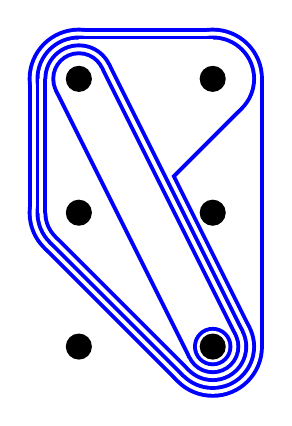
\begin{tikzpicture}
\node[fill] (1) at (0.0, 0.0) [circle] {};
\node[fill] (2) at (1.7, 0.0) [circle] {};
\node[fill] (3) at (0.0, -1.7) [circle] {};
\node[fill] (4) at (1.7, -1.7) [circle] {};
\node[fill] (5) at (0.0, -3.4) [circle] {};
\node[fill] (6) at (1.7, -3.4) [circle] {};
%12346
\begin{scope}[on background layer]
\fill[\tubecolor] (1) circle (\n + 9*\thickness);
\fill[\tubecolor] (2) circle (\n + 9*\thickness);
\fill[\tubecolor] (3) circle (\n + 9*\thickness);
\fill[\tubecolor] (4) circle (\n + 9*\thickness);
\fill[\tubecolor] (6) circle (\n + 9*\thickness);
\draw[\tubecolor] [line width = 2*(\n + 9*\thickness)] (1.center) -- (2.center);
\draw[\tubecolor] [line width = 2*(\n + 9*\thickness)] (1.center) -- (3.center);
\draw[\tubecolor] [line width = 2*(\n + 9*\thickness)] (1.center) -- (4.center);
\draw[\tubecolor] [line width = 2*(\n + 9*\thickness)] (1.center) -- (6.center);
\draw[\tubecolor] [line width = 2*(\n + 9*\thickness)] (2.center) -- (3.center);
\draw[\tubecolor] [line width = 2*(\n + 9*\thickness)] (2.center) -- (4.center);
\draw[\tubecolor] [line width = 2*(\n + 9*\thickness)] (3.center) -- (4.center);
\draw[\tubecolor] [line width = 2*(\n + 9*\thickness)] (3.center) -- (6.center);
\draw[\tubecolor] [line width = 2*(\n + 9*\thickness)] (4.center) -- (6.center);
\draw[white] [line width = 2*(\n + 8*\thickness)] (1.center) -- (2.center);
\draw[white] [line width = 2*(\n + 8*\thickness)] (1.center) -- (3.center);
\draw[white] [line width = 2*(\n + 8*\thickness)] (1.center) -- (4.center);
\draw[white] [line width = 2*(\n + 8*\thickness)] (1.center) -- (6.center);
\draw[white] [line width = 2*(\n + 8*\thickness)] (2.center) -- (3.center);
\draw[white] [line width = 2*(\n + 8*\thickness)] (2.center) -- (4.center);
\draw[white] [line width = 2*(\n + 8*\thickness)] (3.center) -- (4.center);
\draw[white] [line width = 2*(\n + 8*\thickness)] (3.center) -- (6.center);
\draw[white] [line width = 2*(\n + 8*\thickness)] (4.center) -- (6.center);
\fill[white] (1.center) -- (3.center) -- (2.center) -- (1.center);
\fill[white] (2.center) -- (4.center) -- (1.center) -- (2.center);
\fill[white] (1.center) -- (3.center) -- (4.center) -- (1.center);
\fill[white] (1.center) -- (3.center) -- (6.center) -- (1.center);
\fill[white] (4.center) -- (6.center) -- (1.center) -- (4.center);
\fill[white] (2.center) -- (4.center) -- (3.center) -- (2.center);
\fill[white] (4.center) -- (6.center) -- (3.center) -- (4.center);
\fill[white] (1) circle (\n + 8*\thickness);
\fill[white] (2) circle (\n + 8*\thickness);
\fill[white] (3) circle (\n + 8*\thickness);
\fill[white] (4) circle (\n + 8*\thickness);
\fill[white] (6) circle (\n + 8*\thickness);
\end{scope}
%1236
\begin{scope}[on background layer]
\fill[\tubecolor] (1) circle (\n + 7*\thickness);
\fill[\tubecolor] (2) circle (\n + 7*\thickness);
\fill[\tubecolor] (3) circle (\n + 7*\thickness);
\fill[\tubecolor] (6) circle (\n + 7*\thickness);
\draw[\tubecolor] [line width = 2*(\n + 7*\thickness)] (1.center) -- (2.center);
\draw[\tubecolor] [line width = 2*(\n + 7*\thickness)] (1.center) -- (3.center);
\draw[\tubecolor] [line width = 2*(\n + 7*\thickness)] (1.center) -- (6.center);
\draw[\tubecolor] [line width = 2*(\n + 7*\thickness)] (2.center) -- (3.center);
\draw[\tubecolor] [line width = 2*(\n + 7*\thickness)] (3.center) -- (6.center);
\draw[white] [line width = 2*(\n + 6*\thickness)] (1.center) -- (2.center);
\draw[white] [line width = 2*(\n + 6*\thickness)] (1.center) -- (3.center);
\draw[white] [line width = 2*(\n + 6*\thickness)] (1.center) -- (6.center);
\draw[white] [line width = 2*(\n + 6*\thickness)] (2.center) -- (3.center);
\draw[white] [line width = 2*(\n + 6*\thickness)] (3.center) -- (6.center);
\fill[white] (1.center) -- (3.center) -- (2.center) -- (1.center);
\fill[white] (1.center) -- (3.center) -- (6.center) -- (1.center);
\fill[white] (1) circle (\n + 6*\thickness);
\fill[white] (2) circle (\n + 6*\thickness);
\fill[white] (3) circle (\n + 6*\thickness);
\fill[white] (6) circle (\n + 6*\thickness);
\end{scope}
%136
\begin{scope}[on background layer]
\fill[\tubecolor] (1) circle (\n + 5*\thickness);
\fill[\tubecolor] (3) circle (\n + 5*\thickness);
\fill[\tubecolor] (6) circle (\n + 5*\thickness);
\draw[\tubecolor] [line width = 2*(\n + 5*\thickness)] (1.center) -- (3.center);
\draw[\tubecolor] [line width = 2*(\n + 5*\thickness)] (1.center) -- (6.center);
\draw[\tubecolor] [line width = 2*(\n + 5*\thickness)] (3.center) -- (6.center);
\draw[white] [line width = 2*(\n + 4*\thickness)] (1.center) -- (3.center);
\draw[white] [line width = 2*(\n + 4*\thickness)] (1.center) -- (6.center);
\draw[white] [line width = 2*(\n + 4*\thickness)] (3.center) -- (6.center);
\fill[white] (1.center) -- (3.center) -- (6.center) -- (1.center);
\fill[white] (1) circle (\n + 4*\thickness);
\fill[white] (3) circle (\n + 4*\thickness);
\fill[white] (6) circle (\n + 4*\thickness);
\end{scope}
%16
\begin{scope}[on background layer]
\fill[\tubecolor] (1) circle (\n + 3*\thickness);
\fill[\tubecolor] (6) circle (\n + 3*\thickness);
\draw[\tubecolor] [line width = 2*(\n + 3*\thickness)] (1.center) -- (6.center);
\draw[white] [line width = 2*(\n + 2*\thickness)] (1.center) -- (6.center);
\fill[white] (1) circle (\n + 2*\thickness);
\fill[white] (6) circle (\n + 2*\thickness);
\end{scope}
%6
\begin{scope}[on background layer]
\fill[\tubecolor] (6) circle (\n + 1*\thickness);
\fill[white] (6) circle (\n + 0*\thickness);
\end{scope}
\end{tikzpicture}
%631245
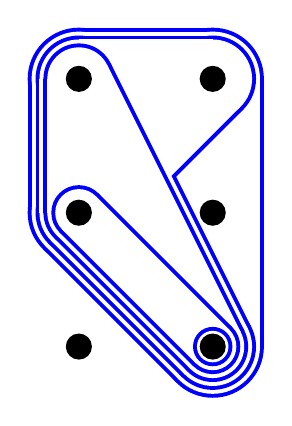
\begin{tikzpicture}
\node[fill] (1) at (0.0, 0.0) [circle] {};
\node[fill] (2) at (1.7, 0.0) [circle] {};
\node[fill] (3) at (0.0, -1.7) [circle] {};
\node[fill] (4) at (1.7, -1.7) [circle] {};
\node[fill] (5) at (0.0, -3.4) [circle] {};
\node[fill] (6) at (1.7, -3.4) [circle] {};
%12346
\begin{scope}[on background layer]
\fill[\tubecolor] (1) circle (\n + 9*\thickness);
\fill[\tubecolor] (2) circle (\n + 9*\thickness);
\fill[\tubecolor] (3) circle (\n + 9*\thickness);
\fill[\tubecolor] (4) circle (\n + 9*\thickness);
\fill[\tubecolor] (6) circle (\n + 9*\thickness);
\draw[\tubecolor] [line width = 2*(\n + 9*\thickness)] (1.center) -- (2.center);
\draw[\tubecolor] [line width = 2*(\n + 9*\thickness)] (1.center) -- (3.center);
\draw[\tubecolor] [line width = 2*(\n + 9*\thickness)] (1.center) -- (4.center);
\draw[\tubecolor] [line width = 2*(\n + 9*\thickness)] (1.center) -- (6.center);
\draw[\tubecolor] [line width = 2*(\n + 9*\thickness)] (2.center) -- (3.center);
\draw[\tubecolor] [line width = 2*(\n + 9*\thickness)] (2.center) -- (4.center);
\draw[\tubecolor] [line width = 2*(\n + 9*\thickness)] (3.center) -- (4.center);
\draw[\tubecolor] [line width = 2*(\n + 9*\thickness)] (3.center) -- (6.center);
\draw[\tubecolor] [line width = 2*(\n + 9*\thickness)] (4.center) -- (6.center);
\draw[white] [line width = 2*(\n + 8*\thickness)] (1.center) -- (2.center);
\draw[white] [line width = 2*(\n + 8*\thickness)] (1.center) -- (3.center);
\draw[white] [line width = 2*(\n + 8*\thickness)] (1.center) -- (4.center);
\draw[white] [line width = 2*(\n + 8*\thickness)] (1.center) -- (6.center);
\draw[white] [line width = 2*(\n + 8*\thickness)] (2.center) -- (3.center);
\draw[white] [line width = 2*(\n + 8*\thickness)] (2.center) -- (4.center);
\draw[white] [line width = 2*(\n + 8*\thickness)] (3.center) -- (4.center);
\draw[white] [line width = 2*(\n + 8*\thickness)] (3.center) -- (6.center);
\draw[white] [line width = 2*(\n + 8*\thickness)] (4.center) -- (6.center);
\fill[white] (1.center) -- (3.center) -- (2.center) -- (1.center);
\fill[white] (2.center) -- (4.center) -- (1.center) -- (2.center);
\fill[white] (1.center) -- (3.center) -- (4.center) -- (1.center);
\fill[white] (1.center) -- (3.center) -- (6.center) -- (1.center);
\fill[white] (4.center) -- (6.center) -- (1.center) -- (4.center);
\fill[white] (2.center) -- (4.center) -- (3.center) -- (2.center);
\fill[white] (4.center) -- (6.center) -- (3.center) -- (4.center);
\fill[white] (1) circle (\n + 8*\thickness);
\fill[white] (2) circle (\n + 8*\thickness);
\fill[white] (3) circle (\n + 8*\thickness);
\fill[white] (4) circle (\n + 8*\thickness);
\fill[white] (6) circle (\n + 8*\thickness);
\end{scope}
%1236
\begin{scope}[on background layer]
\fill[\tubecolor] (1) circle (\n + 7*\thickness);
\fill[\tubecolor] (2) circle (\n + 7*\thickness);
\fill[\tubecolor] (3) circle (\n + 7*\thickness);
\fill[\tubecolor] (6) circle (\n + 7*\thickness);
\draw[\tubecolor] [line width = 2*(\n + 7*\thickness)] (1.center) -- (2.center);
\draw[\tubecolor] [line width = 2*(\n + 7*\thickness)] (1.center) -- (3.center);
\draw[\tubecolor] [line width = 2*(\n + 7*\thickness)] (1.center) -- (6.center);
\draw[\tubecolor] [line width = 2*(\n + 7*\thickness)] (2.center) -- (3.center);
\draw[\tubecolor] [line width = 2*(\n + 7*\thickness)] (3.center) -- (6.center);
\draw[white] [line width = 2*(\n + 6*\thickness)] (1.center) -- (2.center);
\draw[white] [line width = 2*(\n + 6*\thickness)] (1.center) -- (3.center);
\draw[white] [line width = 2*(\n + 6*\thickness)] (1.center) -- (6.center);
\draw[white] [line width = 2*(\n + 6*\thickness)] (2.center) -- (3.center);
\draw[white] [line width = 2*(\n + 6*\thickness)] (3.center) -- (6.center);
\fill[white] (1.center) -- (3.center) -- (2.center) -- (1.center);
\fill[white] (1.center) -- (3.center) -- (6.center) -- (1.center);
\fill[white] (1) circle (\n + 6*\thickness);
\fill[white] (2) circle (\n + 6*\thickness);
\fill[white] (3) circle (\n + 6*\thickness);
\fill[white] (6) circle (\n + 6*\thickness);
\end{scope}
%136
\begin{scope}[on background layer]
\fill[\tubecolor] (1) circle (\n + 5*\thickness);
\fill[\tubecolor] (3) circle (\n + 5*\thickness);
\fill[\tubecolor] (6) circle (\n + 5*\thickness);
\draw[\tubecolor] [line width = 2*(\n + 5*\thickness)] (1.center) -- (3.center);
\draw[\tubecolor] [line width = 2*(\n + 5*\thickness)] (1.center) -- (6.center);
\draw[\tubecolor] [line width = 2*(\n + 5*\thickness)] (3.center) -- (6.center);
\draw[white] [line width = 2*(\n + 4*\thickness)] (1.center) -- (3.center);
\draw[white] [line width = 2*(\n + 4*\thickness)] (1.center) -- (6.center);
\draw[white] [line width = 2*(\n + 4*\thickness)] (3.center) -- (6.center);
\fill[white] (1.center) -- (3.center) -- (6.center) -- (1.center);
\fill[white] (1) circle (\n + 4*\thickness);
\fill[white] (3) circle (\n + 4*\thickness);
\fill[white] (6) circle (\n + 4*\thickness);
\end{scope}
%36
\begin{scope}[on background layer]
\fill[\tubecolor] (3) circle (\n + 3*\thickness);
\fill[\tubecolor] (6) circle (\n + 3*\thickness);
\draw[\tubecolor] [line width = 2*(\n + 3*\thickness)] (3.center) -- (6.center);
\draw[white] [line width = 2*(\n + 2*\thickness)] (3.center) -- (6.center);
\fill[white] (3) circle (\n + 2*\thickness);
\fill[white] (6) circle (\n + 2*\thickness);
\end{scope}
%6
\begin{scope}[on background layer]
\fill[\tubecolor] (6) circle (\n + 1*\thickness);
\fill[white] (6) circle (\n + 0*\thickness);
\end{scope}
\end{tikzpicture}
%632145
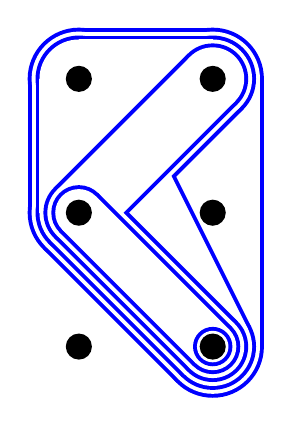
\begin{tikzpicture}
\node[fill] (1) at (0.0, 0.0) [circle] {};
\node[fill] (2) at (1.7, 0.0) [circle] {};
\node[fill] (3) at (0.0, -1.7) [circle] {};
\node[fill] (4) at (1.7, -1.7) [circle] {};
\node[fill] (5) at (0.0, -3.4) [circle] {};
\node[fill] (6) at (1.7, -3.4) [circle] {};
%12346
\begin{scope}[on background layer]
\fill[\tubecolor] (1) circle (\n + 9*\thickness);
\fill[\tubecolor] (2) circle (\n + 9*\thickness);
\fill[\tubecolor] (3) circle (\n + 9*\thickness);
\fill[\tubecolor] (4) circle (\n + 9*\thickness);
\fill[\tubecolor] (6) circle (\n + 9*\thickness);
\draw[\tubecolor] [line width = 2*(\n + 9*\thickness)] (1.center) -- (2.center);
\draw[\tubecolor] [line width = 2*(\n + 9*\thickness)] (1.center) -- (3.center);
\draw[\tubecolor] [line width = 2*(\n + 9*\thickness)] (1.center) -- (4.center);
\draw[\tubecolor] [line width = 2*(\n + 9*\thickness)] (1.center) -- (6.center);
\draw[\tubecolor] [line width = 2*(\n + 9*\thickness)] (2.center) -- (3.center);
\draw[\tubecolor] [line width = 2*(\n + 9*\thickness)] (2.center) -- (4.center);
\draw[\tubecolor] [line width = 2*(\n + 9*\thickness)] (3.center) -- (4.center);
\draw[\tubecolor] [line width = 2*(\n + 9*\thickness)] (3.center) -- (6.center);
\draw[\tubecolor] [line width = 2*(\n + 9*\thickness)] (4.center) -- (6.center);
\draw[white] [line width = 2*(\n + 8*\thickness)] (1.center) -- (2.center);
\draw[white] [line width = 2*(\n + 8*\thickness)] (1.center) -- (3.center);
\draw[white] [line width = 2*(\n + 8*\thickness)] (1.center) -- (4.center);
\draw[white] [line width = 2*(\n + 8*\thickness)] (1.center) -- (6.center);
\draw[white] [line width = 2*(\n + 8*\thickness)] (2.center) -- (3.center);
\draw[white] [line width = 2*(\n + 8*\thickness)] (2.center) -- (4.center);
\draw[white] [line width = 2*(\n + 8*\thickness)] (3.center) -- (4.center);
\draw[white] [line width = 2*(\n + 8*\thickness)] (3.center) -- (6.center);
\draw[white] [line width = 2*(\n + 8*\thickness)] (4.center) -- (6.center);
\fill[white] (1.center) -- (3.center) -- (2.center) -- (1.center);
\fill[white] (2.center) -- (4.center) -- (1.center) -- (2.center);
\fill[white] (1.center) -- (3.center) -- (4.center) -- (1.center);
\fill[white] (1.center) -- (3.center) -- (6.center) -- (1.center);
\fill[white] (4.center) -- (6.center) -- (1.center) -- (4.center);
\fill[white] (2.center) -- (4.center) -- (3.center) -- (2.center);
\fill[white] (4.center) -- (6.center) -- (3.center) -- (4.center);
\fill[white] (1) circle (\n + 8*\thickness);
\fill[white] (2) circle (\n + 8*\thickness);
\fill[white] (3) circle (\n + 8*\thickness);
\fill[white] (4) circle (\n + 8*\thickness);
\fill[white] (6) circle (\n + 8*\thickness);
\end{scope}
%1236
\begin{scope}[on background layer]
\fill[\tubecolor] (1) circle (\n + 7*\thickness);
\fill[\tubecolor] (2) circle (\n + 7*\thickness);
\fill[\tubecolor] (3) circle (\n + 7*\thickness);
\fill[\tubecolor] (6) circle (\n + 7*\thickness);
\draw[\tubecolor] [line width = 2*(\n + 7*\thickness)] (1.center) -- (2.center);
\draw[\tubecolor] [line width = 2*(\n + 7*\thickness)] (1.center) -- (3.center);
\draw[\tubecolor] [line width = 2*(\n + 7*\thickness)] (1.center) -- (6.center);
\draw[\tubecolor] [line width = 2*(\n + 7*\thickness)] (2.center) -- (3.center);
\draw[\tubecolor] [line width = 2*(\n + 7*\thickness)] (3.center) -- (6.center);
\draw[white] [line width = 2*(\n + 6*\thickness)] (1.center) -- (2.center);
\draw[white] [line width = 2*(\n + 6*\thickness)] (1.center) -- (3.center);
\draw[white] [line width = 2*(\n + 6*\thickness)] (1.center) -- (6.center);
\draw[white] [line width = 2*(\n + 6*\thickness)] (2.center) -- (3.center);
\draw[white] [line width = 2*(\n + 6*\thickness)] (3.center) -- (6.center);
\fill[white] (1.center) -- (3.center) -- (2.center) -- (1.center);
\fill[white] (1.center) -- (3.center) -- (6.center) -- (1.center);
\fill[white] (1) circle (\n + 6*\thickness);
\fill[white] (2) circle (\n + 6*\thickness);
\fill[white] (3) circle (\n + 6*\thickness);
\fill[white] (6) circle (\n + 6*\thickness);
\end{scope}
%236
\begin{scope}[on background layer]
\fill[\tubecolor] (2) circle (\n + 5*\thickness);
\fill[\tubecolor] (3) circle (\n + 5*\thickness);
\fill[\tubecolor] (6) circle (\n + 5*\thickness);
\draw[\tubecolor] [line width = 2*(\n + 5*\thickness)] (2.center) -- (3.center);
\draw[\tubecolor] [line width = 2*(\n + 5*\thickness)] (3.center) -- (6.center);
\draw[white] [line width = 2*(\n + 4*\thickness)] (2.center) -- (3.center);
\draw[white] [line width = 2*(\n + 4*\thickness)] (3.center) -- (6.center);
\fill[white] (2) circle (\n + 4*\thickness);
\fill[white] (3) circle (\n + 4*\thickness);
\fill[white] (6) circle (\n + 4*\thickness);
\end{scope}
%36
\begin{scope}[on background layer]
\fill[\tubecolor] (3) circle (\n + 3*\thickness);
\fill[\tubecolor] (6) circle (\n + 3*\thickness);
\draw[\tubecolor] [line width = 2*(\n + 3*\thickness)] (3.center) -- (6.center);
\draw[white] [line width = 2*(\n + 2*\thickness)] (3.center) -- (6.center);
\fill[white] (3) circle (\n + 2*\thickness);
\fill[white] (6) circle (\n + 2*\thickness);
\end{scope}
%6
\begin{scope}[on background layer]
\fill[\tubecolor] (6) circle (\n + 1*\thickness);
\fill[white] (6) circle (\n + 0*\thickness);
\end{scope}
\end{tikzpicture}


%632415
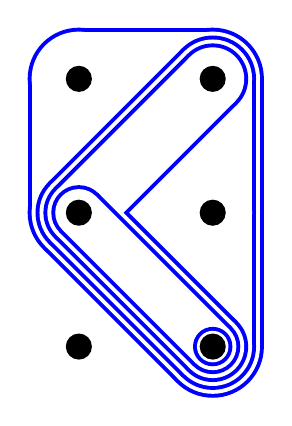
\begin{tikzpicture}
\node[fill] (1) at (0.0, 0.0) [circle] {};
\node[fill] (2) at (1.7, 0.0) [circle] {};
\node[fill] (3) at (0.0, -1.7) [circle] {};
\node[fill] (4) at (1.7, -1.7) [circle] {};
\node[fill] (5) at (0.0, -3.4) [circle] {};
\node[fill] (6) at (1.7, -3.4) [circle] {};
%12346
\begin{scope}[on background layer]
\fill[\tubecolor] (1) circle (\n + 9*\thickness);
\fill[\tubecolor] (2) circle (\n + 9*\thickness);
\fill[\tubecolor] (3) circle (\n + 9*\thickness);
\fill[\tubecolor] (4) circle (\n + 9*\thickness);
\fill[\tubecolor] (6) circle (\n + 9*\thickness);
\draw[\tubecolor] [line width = 2*(\n + 9*\thickness)] (1.center) -- (2.center);
\draw[\tubecolor] [line width = 2*(\n + 9*\thickness)] (1.center) -- (3.center);
\draw[\tubecolor] [line width = 2*(\n + 9*\thickness)] (1.center) -- (4.center);
\draw[\tubecolor] [line width = 2*(\n + 9*\thickness)] (1.center) -- (6.center);
\draw[\tubecolor] [line width = 2*(\n + 9*\thickness)] (2.center) -- (3.center);
\draw[\tubecolor] [line width = 2*(\n + 9*\thickness)] (2.center) -- (4.center);
\draw[\tubecolor] [line width = 2*(\n + 9*\thickness)] (3.center) -- (4.center);
\draw[\tubecolor] [line width = 2*(\n + 9*\thickness)] (3.center) -- (6.center);
\draw[\tubecolor] [line width = 2*(\n + 9*\thickness)] (4.center) -- (6.center);
\draw[white] [line width = 2*(\n + 8*\thickness)] (1.center) -- (2.center);
\draw[white] [line width = 2*(\n + 8*\thickness)] (1.center) -- (3.center);
\draw[white] [line width = 2*(\n + 8*\thickness)] (1.center) -- (4.center);
\draw[white] [line width = 2*(\n + 8*\thickness)] (1.center) -- (6.center);
\draw[white] [line width = 2*(\n + 8*\thickness)] (2.center) -- (3.center);
\draw[white] [line width = 2*(\n + 8*\thickness)] (2.center) -- (4.center);
\draw[white] [line width = 2*(\n + 8*\thickness)] (3.center) -- (4.center);
\draw[white] [line width = 2*(\n + 8*\thickness)] (3.center) -- (6.center);
\draw[white] [line width = 2*(\n + 8*\thickness)] (4.center) -- (6.center);
\fill[white] (1.center) -- (3.center) -- (2.center) -- (1.center);
\fill[white] (2.center) -- (4.center) -- (1.center) -- (2.center);
\fill[white] (1.center) -- (3.center) -- (4.center) -- (1.center);
\fill[white] (1.center) -- (3.center) -- (6.center) -- (1.center);
\fill[white] (4.center) -- (6.center) -- (1.center) -- (4.center);
\fill[white] (2.center) -- (4.center) -- (3.center) -- (2.center);
\fill[white] (4.center) -- (6.center) -- (3.center) -- (4.center);
\fill[white] (1) circle (\n + 8*\thickness);
\fill[white] (2) circle (\n + 8*\thickness);
\fill[white] (3) circle (\n + 8*\thickness);
\fill[white] (4) circle (\n + 8*\thickness);
\fill[white] (6) circle (\n + 8*\thickness);
\end{scope}
%2346
\begin{scope}[on background layer]
\fill[\tubecolor] (2) circle (\n + 7*\thickness);
\fill[\tubecolor] (3) circle (\n + 7*\thickness);
\fill[\tubecolor] (4) circle (\n + 7*\thickness);
\fill[\tubecolor] (6) circle (\n + 7*\thickness);
\draw[\tubecolor] [line width = 2*(\n + 7*\thickness)] (2.center) -- (3.center);
\draw[\tubecolor] [line width = 2*(\n + 7*\thickness)] (2.center) -- (4.center);
\draw[\tubecolor] [line width = 2*(\n + 7*\thickness)] (3.center) -- (4.center);
\draw[\tubecolor] [line width = 2*(\n + 7*\thickness)] (3.center) -- (6.center);
\draw[\tubecolor] [line width = 2*(\n + 7*\thickness)] (4.center) -- (6.center);
\draw[white] [line width = 2*(\n + 6*\thickness)] (2.center) -- (3.center);
\draw[white] [line width = 2*(\n + 6*\thickness)] (2.center) -- (4.center);
\draw[white] [line width = 2*(\n + 6*\thickness)] (3.center) -- (4.center);
\draw[white] [line width = 2*(\n + 6*\thickness)] (3.center) -- (6.center);
\draw[white] [line width = 2*(\n + 6*\thickness)] (4.center) -- (6.center);
\fill[white] (2.center) -- (4.center) -- (3.center) -- (2.center);
\fill[white] (4.center) -- (6.center) -- (3.center) -- (4.center);
\fill[white] (2) circle (\n + 6*\thickness);
\fill[white] (3) circle (\n + 6*\thickness);
\fill[white] (4) circle (\n + 6*\thickness);
\fill[white] (6) circle (\n + 6*\thickness);
\end{scope}
%236
\begin{scope}[on background layer]
\fill[\tubecolor] (2) circle (\n + 5*\thickness);
\fill[\tubecolor] (3) circle (\n + 5*\thickness);
\fill[\tubecolor] (6) circle (\n + 5*\thickness);
\draw[\tubecolor] [line width = 2*(\n + 5*\thickness)] (2.center) -- (3.center);
\draw[\tubecolor] [line width = 2*(\n + 5*\thickness)] (3.center) -- (6.center);
\draw[white] [line width = 2*(\n + 4*\thickness)] (2.center) -- (3.center);
\draw[white] [line width = 2*(\n + 4*\thickness)] (3.center) -- (6.center);
\fill[white] (2) circle (\n + 4*\thickness);
\fill[white] (3) circle (\n + 4*\thickness);
\fill[white] (6) circle (\n + 4*\thickness);
\end{scope}
%36
\begin{scope}[on background layer]
\fill[\tubecolor] (3) circle (\n + 3*\thickness);
\fill[\tubecolor] (6) circle (\n + 3*\thickness);
\draw[\tubecolor] [line width = 2*(\n + 3*\thickness)] (3.center) -- (6.center);
\draw[white] [line width = 2*(\n + 2*\thickness)] (3.center) -- (6.center);
\fill[white] (3) circle (\n + 2*\thickness);
\fill[white] (6) circle (\n + 2*\thickness);
\end{scope}
%6
\begin{scope}[on background layer]
\fill[\tubecolor] (6) circle (\n + 1*\thickness);
\fill[white] (6) circle (\n + 0*\thickness);
\end{scope}
\end{tikzpicture}
%632451
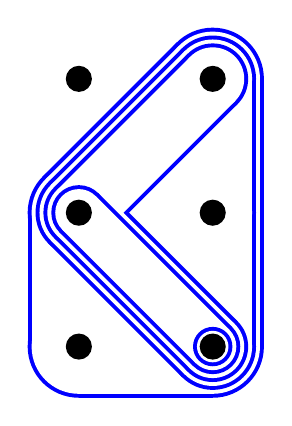
\begin{tikzpicture}
\node[fill] (1) at (0.0, 0.0) [circle] {};
\node[fill] (2) at (1.7, 0.0) [circle] {};
\node[fill] (3) at (0.0, -1.7) [circle] {};
\node[fill] (4) at (1.7, -1.7) [circle] {};
\node[fill] (5) at (0.0, -3.4) [circle] {};
\node[fill] (6) at (1.7, -3.4) [circle] {};
%23456
\begin{scope}[on background layer]
\fill[\tubecolor] (2) circle (\n + 9*\thickness);
\fill[\tubecolor] (3) circle (\n + 9*\thickness);
\fill[\tubecolor] (4) circle (\n + 9*\thickness);
\fill[\tubecolor] (5) circle (\n + 9*\thickness);
\fill[\tubecolor] (6) circle (\n + 9*\thickness);
\draw[\tubecolor] [line width = 2*(\n + 9*\thickness)] (2.center) -- (3.center);
\draw[\tubecolor] [line width = 2*(\n + 9*\thickness)] (2.center) -- (4.center);
\draw[\tubecolor] [line width = 2*(\n + 9*\thickness)] (2.center) -- (5.center);
\draw[\tubecolor] [line width = 2*(\n + 9*\thickness)] (3.center) -- (4.center);
\draw[\tubecolor] [line width = 2*(\n + 9*\thickness)] (3.center) -- (5.center);
\draw[\tubecolor] [line width = 2*(\n + 9*\thickness)] (3.center) -- (6.center);
\draw[\tubecolor] [line width = 2*(\n + 9*\thickness)] (4.center) -- (5.center);
\draw[\tubecolor] [line width = 2*(\n + 9*\thickness)] (4.center) -- (6.center);
\draw[\tubecolor] [line width = 2*(\n + 9*\thickness)] (5.center) -- (6.center);
\draw[white] [line width = 2*(\n + 8*\thickness)] (2.center) -- (3.center);
\draw[white] [line width = 2*(\n + 8*\thickness)] (2.center) -- (4.center);
\draw[white] [line width = 2*(\n + 8*\thickness)] (2.center) -- (5.center);
\draw[white] [line width = 2*(\n + 8*\thickness)] (3.center) -- (4.center);
\draw[white] [line width = 2*(\n + 8*\thickness)] (3.center) -- (5.center);
\draw[white] [line width = 2*(\n + 8*\thickness)] (3.center) -- (6.center);
\draw[white] [line width = 2*(\n + 8*\thickness)] (4.center) -- (5.center);
\draw[white] [line width = 2*(\n + 8*\thickness)] (4.center) -- (6.center);
\draw[white] [line width = 2*(\n + 8*\thickness)] (5.center) -- (6.center);
\fill[white] (2.center) -- (4.center) -- (3.center) -- (2.center);
\fill[white] (3.center) -- (5.center) -- (2.center) -- (3.center);
\fill[white] (2.center) -- (4.center) -- (5.center) -- (2.center);
\fill[white] (3.center) -- (5.center) -- (4.center) -- (3.center);
\fill[white] (4.center) -- (6.center) -- (3.center) -- (4.center);
\fill[white] (3.center) -- (5.center) -- (6.center) -- (3.center);
\fill[white] (4.center) -- (6.center) -- (5.center) -- (4.center);
\fill[white] (2) circle (\n + 8*\thickness);
\fill[white] (3) circle (\n + 8*\thickness);
\fill[white] (4) circle (\n + 8*\thickness);
\fill[white] (5) circle (\n + 8*\thickness);
\fill[white] (6) circle (\n + 8*\thickness);
\end{scope}
%2346
\begin{scope}[on background layer]
\fill[\tubecolor] (2) circle (\n + 7*\thickness);
\fill[\tubecolor] (3) circle (\n + 7*\thickness);
\fill[\tubecolor] (4) circle (\n + 7*\thickness);
\fill[\tubecolor] (6) circle (\n + 7*\thickness);
\draw[\tubecolor] [line width = 2*(\n + 7*\thickness)] (2.center) -- (3.center);
\draw[\tubecolor] [line width = 2*(\n + 7*\thickness)] (2.center) -- (4.center);
\draw[\tubecolor] [line width = 2*(\n + 7*\thickness)] (3.center) -- (4.center);
\draw[\tubecolor] [line width = 2*(\n + 7*\thickness)] (3.center) -- (6.center);
\draw[\tubecolor] [line width = 2*(\n + 7*\thickness)] (4.center) -- (6.center);
\draw[white] [line width = 2*(\n + 6*\thickness)] (2.center) -- (3.center);
\draw[white] [line width = 2*(\n + 6*\thickness)] (2.center) -- (4.center);
\draw[white] [line width = 2*(\n + 6*\thickness)] (3.center) -- (4.center);
\draw[white] [line width = 2*(\n + 6*\thickness)] (3.center) -- (6.center);
\draw[white] [line width = 2*(\n + 6*\thickness)] (4.center) -- (6.center);
\fill[white] (2.center) -- (4.center) -- (3.center) -- (2.center);
\fill[white] (4.center) -- (6.center) -- (3.center) -- (4.center);
\fill[white] (2) circle (\n + 6*\thickness);
\fill[white] (3) circle (\n + 6*\thickness);
\fill[white] (4) circle (\n + 6*\thickness);
\fill[white] (6) circle (\n + 6*\thickness);
\end{scope}
%236
\begin{scope}[on background layer]
\fill[\tubecolor] (2) circle (\n + 5*\thickness);
\fill[\tubecolor] (3) circle (\n + 5*\thickness);
\fill[\tubecolor] (6) circle (\n + 5*\thickness);
\draw[\tubecolor] [line width = 2*(\n + 5*\thickness)] (2.center) -- (3.center);
\draw[\tubecolor] [line width = 2*(\n + 5*\thickness)] (3.center) -- (6.center);
\draw[white] [line width = 2*(\n + 4*\thickness)] (2.center) -- (3.center);
\draw[white] [line width = 2*(\n + 4*\thickness)] (3.center) -- (6.center);
\fill[white] (2) circle (\n + 4*\thickness);
\fill[white] (3) circle (\n + 4*\thickness);
\fill[white] (6) circle (\n + 4*\thickness);
\end{scope}
%36
\begin{scope}[on background layer]
\fill[\tubecolor] (3) circle (\n + 3*\thickness);
\fill[\tubecolor] (6) circle (\n + 3*\thickness);
\draw[\tubecolor] [line width = 2*(\n + 3*\thickness)] (3.center) -- (6.center);
\draw[white] [line width = 2*(\n + 2*\thickness)] (3.center) -- (6.center);
\fill[white] (3) circle (\n + 2*\thickness);
\fill[white] (6) circle (\n + 2*\thickness);
\end{scope}
%6
\begin{scope}[on background layer]
\fill[\tubecolor] (6) circle (\n + 1*\thickness);
\fill[white] (6) circle (\n + 0*\thickness);
\end{scope}
\end{tikzpicture}
%634251
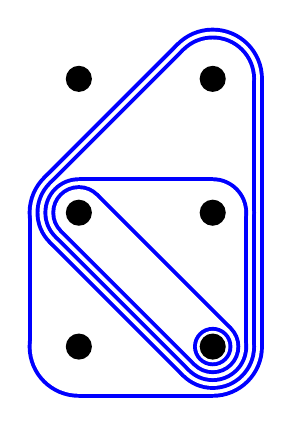
\begin{tikzpicture}
\node[fill] (1) at (0.0, 0.0) [circle] {};
\node[fill] (2) at (1.7, 0.0) [circle] {};
\node[fill] (3) at (0.0, -1.7) [circle] {};
\node[fill] (4) at (1.7, -1.7) [circle] {};
\node[fill] (5) at (0.0, -3.4) [circle] {};
\node[fill] (6) at (1.7, -3.4) [circle] {};
%23456
\begin{scope}[on background layer]
\fill[\tubecolor] (2) circle (\n + 9*\thickness);
\fill[\tubecolor] (3) circle (\n + 9*\thickness);
\fill[\tubecolor] (4) circle (\n + 9*\thickness);
\fill[\tubecolor] (5) circle (\n + 9*\thickness);
\fill[\tubecolor] (6) circle (\n + 9*\thickness);
\draw[\tubecolor] [line width = 2*(\n + 9*\thickness)] (2.center) -- (3.center);
\draw[\tubecolor] [line width = 2*(\n + 9*\thickness)] (2.center) -- (4.center);
\draw[\tubecolor] [line width = 2*(\n + 9*\thickness)] (2.center) -- (5.center);
\draw[\tubecolor] [line width = 2*(\n + 9*\thickness)] (3.center) -- (4.center);
\draw[\tubecolor] [line width = 2*(\n + 9*\thickness)] (3.center) -- (5.center);
\draw[\tubecolor] [line width = 2*(\n + 9*\thickness)] (3.center) -- (6.center);
\draw[\tubecolor] [line width = 2*(\n + 9*\thickness)] (4.center) -- (5.center);
\draw[\tubecolor] [line width = 2*(\n + 9*\thickness)] (4.center) -- (6.center);
\draw[\tubecolor] [line width = 2*(\n + 9*\thickness)] (5.center) -- (6.center);
\draw[white] [line width = 2*(\n + 8*\thickness)] (2.center) -- (3.center);
\draw[white] [line width = 2*(\n + 8*\thickness)] (2.center) -- (4.center);
\draw[white] [line width = 2*(\n + 8*\thickness)] (2.center) -- (5.center);
\draw[white] [line width = 2*(\n + 8*\thickness)] (3.center) -- (4.center);
\draw[white] [line width = 2*(\n + 8*\thickness)] (3.center) -- (5.center);
\draw[white] [line width = 2*(\n + 8*\thickness)] (3.center) -- (6.center);
\draw[white] [line width = 2*(\n + 8*\thickness)] (4.center) -- (5.center);
\draw[white] [line width = 2*(\n + 8*\thickness)] (4.center) -- (6.center);
\draw[white] [line width = 2*(\n + 8*\thickness)] (5.center) -- (6.center);
\fill[white] (2.center) -- (4.center) -- (3.center) -- (2.center);
\fill[white] (3.center) -- (5.center) -- (2.center) -- (3.center);
\fill[white] (2.center) -- (4.center) -- (5.center) -- (2.center);
\fill[white] (3.center) -- (5.center) -- (4.center) -- (3.center);
\fill[white] (4.center) -- (6.center) -- (3.center) -- (4.center);
\fill[white] (3.center) -- (5.center) -- (6.center) -- (3.center);
\fill[white] (4.center) -- (6.center) -- (5.center) -- (4.center);
\fill[white] (2) circle (\n + 8*\thickness);
\fill[white] (3) circle (\n + 8*\thickness);
\fill[white] (4) circle (\n + 8*\thickness);
\fill[white] (5) circle (\n + 8*\thickness);
\fill[white] (6) circle (\n + 8*\thickness);
\end{scope}
%2346
\begin{scope}[on background layer]
\fill[\tubecolor] (2) circle (\n + 7*\thickness);
\fill[\tubecolor] (3) circle (\n + 7*\thickness);
\fill[\tubecolor] (4) circle (\n + 7*\thickness);
\fill[\tubecolor] (6) circle (\n + 7*\thickness);
\draw[\tubecolor] [line width = 2*(\n + 7*\thickness)] (2.center) -- (3.center);
\draw[\tubecolor] [line width = 2*(\n + 7*\thickness)] (2.center) -- (4.center);
\draw[\tubecolor] [line width = 2*(\n + 7*\thickness)] (3.center) -- (4.center);
\draw[\tubecolor] [line width = 2*(\n + 7*\thickness)] (3.center) -- (6.center);
\draw[\tubecolor] [line width = 2*(\n + 7*\thickness)] (4.center) -- (6.center);
\draw[white] [line width = 2*(\n + 6*\thickness)] (2.center) -- (3.center);
\draw[white] [line width = 2*(\n + 6*\thickness)] (2.center) -- (4.center);
\draw[white] [line width = 2*(\n + 6*\thickness)] (3.center) -- (4.center);
\draw[white] [line width = 2*(\n + 6*\thickness)] (3.center) -- (6.center);
\draw[white] [line width = 2*(\n + 6*\thickness)] (4.center) -- (6.center);
\fill[white] (2.center) -- (4.center) -- (3.center) -- (2.center);
\fill[white] (4.center) -- (6.center) -- (3.center) -- (4.center);
\fill[white] (2) circle (\n + 6*\thickness);
\fill[white] (3) circle (\n + 6*\thickness);
\fill[white] (4) circle (\n + 6*\thickness);
\fill[white] (6) circle (\n + 6*\thickness);
\end{scope}
%346
\begin{scope}[on background layer]
\fill[\tubecolor] (3) circle (\n + 5*\thickness);
\fill[\tubecolor] (4) circle (\n + 5*\thickness);
\fill[\tubecolor] (6) circle (\n + 5*\thickness);
\draw[\tubecolor] [line width = 2*(\n + 5*\thickness)] (3.center) -- (4.center);
\draw[\tubecolor] [line width = 2*(\n + 5*\thickness)] (3.center) -- (6.center);
\draw[\tubecolor] [line width = 2*(\n + 5*\thickness)] (4.center) -- (6.center);
\draw[white] [line width = 2*(\n + 4*\thickness)] (3.center) -- (4.center);
\draw[white] [line width = 2*(\n + 4*\thickness)] (3.center) -- (6.center);
\draw[white] [line width = 2*(\n + 4*\thickness)] (4.center) -- (6.center);
\fill[white] (4.center) -- (6.center) -- (3.center) -- (4.center);
\fill[white] (3) circle (\n + 4*\thickness);
\fill[white] (4) circle (\n + 4*\thickness);
\fill[white] (6) circle (\n + 4*\thickness);
\end{scope}
%36
\begin{scope}[on background layer]
\fill[\tubecolor] (3) circle (\n + 3*\thickness);
\fill[\tubecolor] (6) circle (\n + 3*\thickness);
\draw[\tubecolor] [line width = 2*(\n + 3*\thickness)] (3.center) -- (6.center);
\draw[white] [line width = 2*(\n + 2*\thickness)] (3.center) -- (6.center);
\fill[white] (3) circle (\n + 2*\thickness);
\fill[white] (6) circle (\n + 2*\thickness);
\end{scope}
%6
\begin{scope}[on background layer]
\fill[\tubecolor] (6) circle (\n + 1*\thickness);
\fill[white] (6) circle (\n + 0*\thickness);
\end{scope}
\end{tikzpicture}
%634521
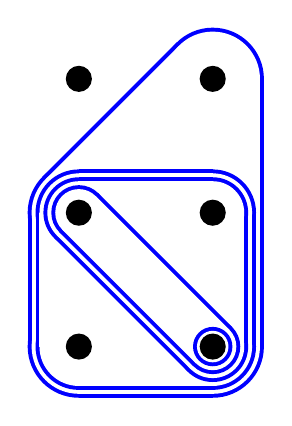
\begin{tikzpicture}
\node[fill] (1) at (0.0, 0.0) [circle] {};
\node[fill] (2) at (1.7, 0.0) [circle] {};
\node[fill] (3) at (0.0, -1.7) [circle] {};
\node[fill] (4) at (1.7, -1.7) [circle] {};
\node[fill] (5) at (0.0, -3.4) [circle] {};
\node[fill] (6) at (1.7, -3.4) [circle] {};
%23456
\begin{scope}[on background layer]
\fill[\tubecolor] (2) circle (\n + 9*\thickness);
\fill[\tubecolor] (3) circle (\n + 9*\thickness);
\fill[\tubecolor] (4) circle (\n + 9*\thickness);
\fill[\tubecolor] (5) circle (\n + 9*\thickness);
\fill[\tubecolor] (6) circle (\n + 9*\thickness);
\draw[\tubecolor] [line width = 2*(\n + 9*\thickness)] (2.center) -- (3.center);
\draw[\tubecolor] [line width = 2*(\n + 9*\thickness)] (2.center) -- (4.center);
\draw[\tubecolor] [line width = 2*(\n + 9*\thickness)] (2.center) -- (5.center);
\draw[\tubecolor] [line width = 2*(\n + 9*\thickness)] (3.center) -- (4.center);
\draw[\tubecolor] [line width = 2*(\n + 9*\thickness)] (3.center) -- (5.center);
\draw[\tubecolor] [line width = 2*(\n + 9*\thickness)] (3.center) -- (6.center);
\draw[\tubecolor] [line width = 2*(\n + 9*\thickness)] (4.center) -- (5.center);
\draw[\tubecolor] [line width = 2*(\n + 9*\thickness)] (4.center) -- (6.center);
\draw[\tubecolor] [line width = 2*(\n + 9*\thickness)] (5.center) -- (6.center);
\draw[white] [line width = 2*(\n + 8*\thickness)] (2.center) -- (3.center);
\draw[white] [line width = 2*(\n + 8*\thickness)] (2.center) -- (4.center);
\draw[white] [line width = 2*(\n + 8*\thickness)] (2.center) -- (5.center);
\draw[white] [line width = 2*(\n + 8*\thickness)] (3.center) -- (4.center);
\draw[white] [line width = 2*(\n + 8*\thickness)] (3.center) -- (5.center);
\draw[white] [line width = 2*(\n + 8*\thickness)] (3.center) -- (6.center);
\draw[white] [line width = 2*(\n + 8*\thickness)] (4.center) -- (5.center);
\draw[white] [line width = 2*(\n + 8*\thickness)] (4.center) -- (6.center);
\draw[white] [line width = 2*(\n + 8*\thickness)] (5.center) -- (6.center);
\fill[white] (2.center) -- (4.center) -- (3.center) -- (2.center);
\fill[white] (3.center) -- (5.center) -- (2.center) -- (3.center);
\fill[white] (2.center) -- (4.center) -- (5.center) -- (2.center);
\fill[white] (3.center) -- (5.center) -- (4.center) -- (3.center);
\fill[white] (4.center) -- (6.center) -- (3.center) -- (4.center);
\fill[white] (3.center) -- (5.center) -- (6.center) -- (3.center);
\fill[white] (4.center) -- (6.center) -- (5.center) -- (4.center);
\fill[white] (2) circle (\n + 8*\thickness);
\fill[white] (3) circle (\n + 8*\thickness);
\fill[white] (4) circle (\n + 8*\thickness);
\fill[white] (5) circle (\n + 8*\thickness);
\fill[white] (6) circle (\n + 8*\thickness);
\end{scope}
%3456
\begin{scope}[on background layer]
\fill[\tubecolor] (3) circle (\n + 7*\thickness);
\fill[\tubecolor] (4) circle (\n + 7*\thickness);
\fill[\tubecolor] (5) circle (\n + 7*\thickness);
\fill[\tubecolor] (6) circle (\n + 7*\thickness);
\draw[\tubecolor] [line width = 2*(\n + 7*\thickness)] (3.center) -- (4.center);
\draw[\tubecolor] [line width = 2*(\n + 7*\thickness)] (3.center) -- (5.center);
\draw[\tubecolor] [line width = 2*(\n + 7*\thickness)] (3.center) -- (6.center);
\draw[\tubecolor] [line width = 2*(\n + 7*\thickness)] (4.center) -- (5.center);
\draw[\tubecolor] [line width = 2*(\n + 7*\thickness)] (4.center) -- (6.center);
\draw[\tubecolor] [line width = 2*(\n + 7*\thickness)] (5.center) -- (6.center);
\draw[white] [line width = 2*(\n + 6*\thickness)] (3.center) -- (4.center);
\draw[white] [line width = 2*(\n + 6*\thickness)] (3.center) -- (5.center);
\draw[white] [line width = 2*(\n + 6*\thickness)] (3.center) -- (6.center);
\draw[white] [line width = 2*(\n + 6*\thickness)] (4.center) -- (5.center);
\draw[white] [line width = 2*(\n + 6*\thickness)] (4.center) -- (6.center);
\draw[white] [line width = 2*(\n + 6*\thickness)] (5.center) -- (6.center);
\fill[white] (3.center) -- (5.center) -- (4.center) -- (3.center);
\fill[white] (4.center) -- (6.center) -- (3.center) -- (4.center);
\fill[white] (3.center) -- (5.center) -- (6.center) -- (3.center);
\fill[white] (4.center) -- (6.center) -- (5.center) -- (4.center);
\fill[white] (3) circle (\n + 6*\thickness);
\fill[white] (4) circle (\n + 6*\thickness);
\fill[white] (5) circle (\n + 6*\thickness);
\fill[white] (6) circle (\n + 6*\thickness);
\end{scope}
%346
\begin{scope}[on background layer]
\fill[\tubecolor] (3) circle (\n + 5*\thickness);
\fill[\tubecolor] (4) circle (\n + 5*\thickness);
\fill[\tubecolor] (6) circle (\n + 5*\thickness);
\draw[\tubecolor] [line width = 2*(\n + 5*\thickness)] (3.center) -- (4.center);
\draw[\tubecolor] [line width = 2*(\n + 5*\thickness)] (3.center) -- (6.center);
\draw[\tubecolor] [line width = 2*(\n + 5*\thickness)] (4.center) -- (6.center);
\draw[white] [line width = 2*(\n + 4*\thickness)] (3.center) -- (4.center);
\draw[white] [line width = 2*(\n + 4*\thickness)] (3.center) -- (6.center);
\draw[white] [line width = 2*(\n + 4*\thickness)] (4.center) -- (6.center);
\fill[white] (4.center) -- (6.center) -- (3.center) -- (4.center);
\fill[white] (3) circle (\n + 4*\thickness);
\fill[white] (4) circle (\n + 4*\thickness);
\fill[white] (6) circle (\n + 4*\thickness);
\end{scope}
%36
\begin{scope}[on background layer]
\fill[\tubecolor] (3) circle (\n + 3*\thickness);
\fill[\tubecolor] (6) circle (\n + 3*\thickness);
\draw[\tubecolor] [line width = 2*(\n + 3*\thickness)] (3.center) -- (6.center);
\draw[white] [line width = 2*(\n + 2*\thickness)] (3.center) -- (6.center);
\fill[white] (3) circle (\n + 2*\thickness);
\fill[white] (6) circle (\n + 2*\thickness);
\end{scope}
%6
\begin{scope}[on background layer]
\fill[\tubecolor] (6) circle (\n + 1*\thickness);
\fill[white] (6) circle (\n + 0*\thickness);
\end{scope}
\end{tikzpicture}
%635421
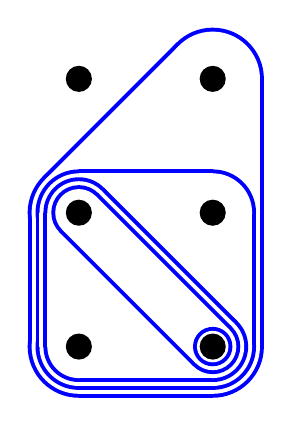
\begin{tikzpicture}
\node[fill] (1) at (0.0, 0.0) [circle] {};
\node[fill] (2) at (1.7, 0.0) [circle] {};
\node[fill] (3) at (0.0, -1.7) [circle] {};
\node[fill] (4) at (1.7, -1.7) [circle] {};
\node[fill] (5) at (0.0, -3.4) [circle] {};
\node[fill] (6) at (1.7, -3.4) [circle] {};
%23456
\begin{scope}[on background layer]
\fill[\tubecolor] (2) circle (\n + 9*\thickness);
\fill[\tubecolor] (3) circle (\n + 9*\thickness);
\fill[\tubecolor] (4) circle (\n + 9*\thickness);
\fill[\tubecolor] (5) circle (\n + 9*\thickness);
\fill[\tubecolor] (6) circle (\n + 9*\thickness);
\draw[\tubecolor] [line width = 2*(\n + 9*\thickness)] (2.center) -- (3.center);
\draw[\tubecolor] [line width = 2*(\n + 9*\thickness)] (2.center) -- (4.center);
\draw[\tubecolor] [line width = 2*(\n + 9*\thickness)] (2.center) -- (5.center);
\draw[\tubecolor] [line width = 2*(\n + 9*\thickness)] (3.center) -- (4.center);
\draw[\tubecolor] [line width = 2*(\n + 9*\thickness)] (3.center) -- (5.center);
\draw[\tubecolor] [line width = 2*(\n + 9*\thickness)] (3.center) -- (6.center);
\draw[\tubecolor] [line width = 2*(\n + 9*\thickness)] (4.center) -- (5.center);
\draw[\tubecolor] [line width = 2*(\n + 9*\thickness)] (4.center) -- (6.center);
\draw[\tubecolor] [line width = 2*(\n + 9*\thickness)] (5.center) -- (6.center);
\draw[white] [line width = 2*(\n + 8*\thickness)] (2.center) -- (3.center);
\draw[white] [line width = 2*(\n + 8*\thickness)] (2.center) -- (4.center);
\draw[white] [line width = 2*(\n + 8*\thickness)] (2.center) -- (5.center);
\draw[white] [line width = 2*(\n + 8*\thickness)] (3.center) -- (4.center);
\draw[white] [line width = 2*(\n + 8*\thickness)] (3.center) -- (5.center);
\draw[white] [line width = 2*(\n + 8*\thickness)] (3.center) -- (6.center);
\draw[white] [line width = 2*(\n + 8*\thickness)] (4.center) -- (5.center);
\draw[white] [line width = 2*(\n + 8*\thickness)] (4.center) -- (6.center);
\draw[white] [line width = 2*(\n + 8*\thickness)] (5.center) -- (6.center);
\fill[white] (2.center) -- (4.center) -- (3.center) -- (2.center);
\fill[white] (3.center) -- (5.center) -- (2.center) -- (3.center);
\fill[white] (2.center) -- (4.center) -- (5.center) -- (2.center);
\fill[white] (3.center) -- (5.center) -- (4.center) -- (3.center);
\fill[white] (4.center) -- (6.center) -- (3.center) -- (4.center);
\fill[white] (3.center) -- (5.center) -- (6.center) -- (3.center);
\fill[white] (4.center) -- (6.center) -- (5.center) -- (4.center);
\fill[white] (2) circle (\n + 8*\thickness);
\fill[white] (3) circle (\n + 8*\thickness);
\fill[white] (4) circle (\n + 8*\thickness);
\fill[white] (5) circle (\n + 8*\thickness);
\fill[white] (6) circle (\n + 8*\thickness);
\end{scope}
%3456
\begin{scope}[on background layer]
\fill[\tubecolor] (3) circle (\n + 7*\thickness);
\fill[\tubecolor] (4) circle (\n + 7*\thickness);
\fill[\tubecolor] (5) circle (\n + 7*\thickness);
\fill[\tubecolor] (6) circle (\n + 7*\thickness);
\draw[\tubecolor] [line width = 2*(\n + 7*\thickness)] (3.center) -- (4.center);
\draw[\tubecolor] [line width = 2*(\n + 7*\thickness)] (3.center) -- (5.center);
\draw[\tubecolor] [line width = 2*(\n + 7*\thickness)] (3.center) -- (6.center);
\draw[\tubecolor] [line width = 2*(\n + 7*\thickness)] (4.center) -- (5.center);
\draw[\tubecolor] [line width = 2*(\n + 7*\thickness)] (4.center) -- (6.center);
\draw[\tubecolor] [line width = 2*(\n + 7*\thickness)] (5.center) -- (6.center);
\draw[white] [line width = 2*(\n + 6*\thickness)] (3.center) -- (4.center);
\draw[white] [line width = 2*(\n + 6*\thickness)] (3.center) -- (5.center);
\draw[white] [line width = 2*(\n + 6*\thickness)] (3.center) -- (6.center);
\draw[white] [line width = 2*(\n + 6*\thickness)] (4.center) -- (5.center);
\draw[white] [line width = 2*(\n + 6*\thickness)] (4.center) -- (6.center);
\draw[white] [line width = 2*(\n + 6*\thickness)] (5.center) -- (6.center);
\fill[white] (3.center) -- (5.center) -- (4.center) -- (3.center);
\fill[white] (4.center) -- (6.center) -- (3.center) -- (4.center);
\fill[white] (3.center) -- (5.center) -- (6.center) -- (3.center);
\fill[white] (4.center) -- (6.center) -- (5.center) -- (4.center);
\fill[white] (3) circle (\n + 6*\thickness);
\fill[white] (4) circle (\n + 6*\thickness);
\fill[white] (5) circle (\n + 6*\thickness);
\fill[white] (6) circle (\n + 6*\thickness);
\end{scope}
%356
\begin{scope}[on background layer]
\fill[\tubecolor] (3) circle (\n + 5*\thickness);
\fill[\tubecolor] (5) circle (\n + 5*\thickness);
\fill[\tubecolor] (6) circle (\n + 5*\thickness);
\draw[\tubecolor] [line width = 2*(\n + 5*\thickness)] (3.center) -- (5.center);
\draw[\tubecolor] [line width = 2*(\n + 5*\thickness)] (3.center) -- (6.center);
\draw[\tubecolor] [line width = 2*(\n + 5*\thickness)] (5.center) -- (6.center);
\draw[white] [line width = 2*(\n + 4*\thickness)] (3.center) -- (5.center);
\draw[white] [line width = 2*(\n + 4*\thickness)] (3.center) -- (6.center);
\draw[white] [line width = 2*(\n + 4*\thickness)] (5.center) -- (6.center);
\fill[white] (3.center) -- (5.center) -- (6.center) -- (3.center);
\fill[white] (3) circle (\n + 4*\thickness);
\fill[white] (5) circle (\n + 4*\thickness);
\fill[white] (6) circle (\n + 4*\thickness);
\end{scope}
%36
\begin{scope}[on background layer]
\fill[\tubecolor] (3) circle (\n + 3*\thickness);
\fill[\tubecolor] (6) circle (\n + 3*\thickness);
\draw[\tubecolor] [line width = 2*(\n + 3*\thickness)] (3.center) -- (6.center);
\draw[white] [line width = 2*(\n + 2*\thickness)] (3.center) -- (6.center);
\fill[white] (3) circle (\n + 2*\thickness);
\fill[white] (6) circle (\n + 2*\thickness);
\end{scope}
%6
\begin{scope}[on background layer]
\fill[\tubecolor] (6) circle (\n + 1*\thickness);
\fill[white] (6) circle (\n + 0*\thickness);
\end{scope}
\end{tikzpicture}
%653421
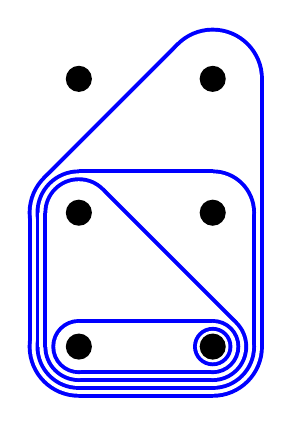
\begin{tikzpicture}
\node[fill] (1) at (0.0, 0.0) [circle] {};
\node[fill] (2) at (1.7, 0.0) [circle] {};
\node[fill] (3) at (0.0, -1.7) [circle] {};
\node[fill] (4) at (1.7, -1.7) [circle] {};
\node[fill] (5) at (0.0, -3.4) [circle] {};
\node[fill] (6) at (1.7, -3.4) [circle] {};
%23456
\begin{scope}[on background layer]
\fill[\tubecolor] (2) circle (\n + 9*\thickness);
\fill[\tubecolor] (3) circle (\n + 9*\thickness);
\fill[\tubecolor] (4) circle (\n + 9*\thickness);
\fill[\tubecolor] (5) circle (\n + 9*\thickness);
\fill[\tubecolor] (6) circle (\n + 9*\thickness);
\draw[\tubecolor] [line width = 2*(\n + 9*\thickness)] (2.center) -- (3.center);
\draw[\tubecolor] [line width = 2*(\n + 9*\thickness)] (2.center) -- (4.center);
\draw[\tubecolor] [line width = 2*(\n + 9*\thickness)] (2.center) -- (5.center);
\draw[\tubecolor] [line width = 2*(\n + 9*\thickness)] (3.center) -- (4.center);
\draw[\tubecolor] [line width = 2*(\n + 9*\thickness)] (3.center) -- (5.center);
\draw[\tubecolor] [line width = 2*(\n + 9*\thickness)] (3.center) -- (6.center);
\draw[\tubecolor] [line width = 2*(\n + 9*\thickness)] (4.center) -- (5.center);
\draw[\tubecolor] [line width = 2*(\n + 9*\thickness)] (4.center) -- (6.center);
\draw[\tubecolor] [line width = 2*(\n + 9*\thickness)] (5.center) -- (6.center);
\draw[white] [line width = 2*(\n + 8*\thickness)] (2.center) -- (3.center);
\draw[white] [line width = 2*(\n + 8*\thickness)] (2.center) -- (4.center);
\draw[white] [line width = 2*(\n + 8*\thickness)] (2.center) -- (5.center);
\draw[white] [line width = 2*(\n + 8*\thickness)] (3.center) -- (4.center);
\draw[white] [line width = 2*(\n + 8*\thickness)] (3.center) -- (5.center);
\draw[white] [line width = 2*(\n + 8*\thickness)] (3.center) -- (6.center);
\draw[white] [line width = 2*(\n + 8*\thickness)] (4.center) -- (5.center);
\draw[white] [line width = 2*(\n + 8*\thickness)] (4.center) -- (6.center);
\draw[white] [line width = 2*(\n + 8*\thickness)] (5.center) -- (6.center);
\fill[white] (2.center) -- (4.center) -- (3.center) -- (2.center);
\fill[white] (3.center) -- (5.center) -- (2.center) -- (3.center);
\fill[white] (2.center) -- (4.center) -- (5.center) -- (2.center);
\fill[white] (3.center) -- (5.center) -- (4.center) -- (3.center);
\fill[white] (4.center) -- (6.center) -- (3.center) -- (4.center);
\fill[white] (3.center) -- (5.center) -- (6.center) -- (3.center);
\fill[white] (4.center) -- (6.center) -- (5.center) -- (4.center);
\fill[white] (2) circle (\n + 8*\thickness);
\fill[white] (3) circle (\n + 8*\thickness);
\fill[white] (4) circle (\n + 8*\thickness);
\fill[white] (5) circle (\n + 8*\thickness);
\fill[white] (6) circle (\n + 8*\thickness);
\end{scope}
%3456
\begin{scope}[on background layer]
\fill[\tubecolor] (3) circle (\n + 7*\thickness);
\fill[\tubecolor] (4) circle (\n + 7*\thickness);
\fill[\tubecolor] (5) circle (\n + 7*\thickness);
\fill[\tubecolor] (6) circle (\n + 7*\thickness);
\draw[\tubecolor] [line width = 2*(\n + 7*\thickness)] (3.center) -- (4.center);
\draw[\tubecolor] [line width = 2*(\n + 7*\thickness)] (3.center) -- (5.center);
\draw[\tubecolor] [line width = 2*(\n + 7*\thickness)] (3.center) -- (6.center);
\draw[\tubecolor] [line width = 2*(\n + 7*\thickness)] (4.center) -- (5.center);
\draw[\tubecolor] [line width = 2*(\n + 7*\thickness)] (4.center) -- (6.center);
\draw[\tubecolor] [line width = 2*(\n + 7*\thickness)] (5.center) -- (6.center);
\draw[white] [line width = 2*(\n + 6*\thickness)] (3.center) -- (4.center);
\draw[white] [line width = 2*(\n + 6*\thickness)] (3.center) -- (5.center);
\draw[white] [line width = 2*(\n + 6*\thickness)] (3.center) -- (6.center);
\draw[white] [line width = 2*(\n + 6*\thickness)] (4.center) -- (5.center);
\draw[white] [line width = 2*(\n + 6*\thickness)] (4.center) -- (6.center);
\draw[white] [line width = 2*(\n + 6*\thickness)] (5.center) -- (6.center);
\fill[white] (3.center) -- (5.center) -- (4.center) -- (3.center);
\fill[white] (4.center) -- (6.center) -- (3.center) -- (4.center);
\fill[white] (3.center) -- (5.center) -- (6.center) -- (3.center);
\fill[white] (4.center) -- (6.center) -- (5.center) -- (4.center);
\fill[white] (3) circle (\n + 6*\thickness);
\fill[white] (4) circle (\n + 6*\thickness);
\fill[white] (5) circle (\n + 6*\thickness);
\fill[white] (6) circle (\n + 6*\thickness);
\end{scope}
%356
\begin{scope}[on background layer]
\fill[\tubecolor] (3) circle (\n + 5*\thickness);
\fill[\tubecolor] (5) circle (\n + 5*\thickness);
\fill[\tubecolor] (6) circle (\n + 5*\thickness);
\draw[\tubecolor] [line width = 2*(\n + 5*\thickness)] (3.center) -- (5.center);
\draw[\tubecolor] [line width = 2*(\n + 5*\thickness)] (3.center) -- (6.center);
\draw[\tubecolor] [line width = 2*(\n + 5*\thickness)] (5.center) -- (6.center);
\draw[white] [line width = 2*(\n + 4*\thickness)] (3.center) -- (5.center);
\draw[white] [line width = 2*(\n + 4*\thickness)] (3.center) -- (6.center);
\draw[white] [line width = 2*(\n + 4*\thickness)] (5.center) -- (6.center);
\fill[white] (3.center) -- (5.center) -- (6.center) -- (3.center);
\fill[white] (3) circle (\n + 4*\thickness);
\fill[white] (5) circle (\n + 4*\thickness);
\fill[white] (6) circle (\n + 4*\thickness);
\end{scope}
%56
\begin{scope}[on background layer]
\fill[\tubecolor] (5) circle (\n + 3*\thickness);
\fill[\tubecolor] (6) circle (\n + 3*\thickness);
\draw[\tubecolor] [line width = 2*(\n + 3*\thickness)] (5.center) -- (6.center);
\draw[white] [line width = 2*(\n + 2*\thickness)] (5.center) -- (6.center);
\fill[white] (5) circle (\n + 2*\thickness);
\fill[white] (6) circle (\n + 2*\thickness);
\end{scope}
%6
\begin{scope}[on background layer]
\fill[\tubecolor] (6) circle (\n + 1*\thickness);
\fill[white] (6) circle (\n + 0*\thickness);
\end{scope}
\end{tikzpicture}
%654321
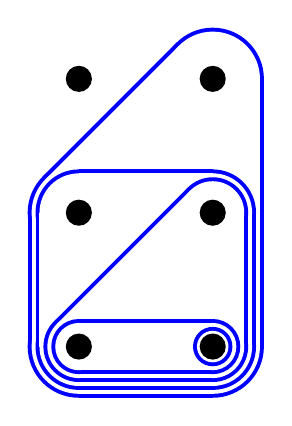
\begin{tikzpicture}
\node[fill] (1) at (0.0, 0.0) [circle] {};
\node[fill] (2) at (1.7, 0.0) [circle] {};
\node[fill] (3) at (0.0, -1.7) [circle] {};
\node[fill] (4) at (1.7, -1.7) [circle] {};
\node[fill] (5) at (0.0, -3.4) [circle] {};
\node[fill] (6) at (1.7, -3.4) [circle] {};
%23456
\begin{scope}[on background layer]
\fill[\tubecolor] (2) circle (\n + 9*\thickness);
\fill[\tubecolor] (3) circle (\n + 9*\thickness);
\fill[\tubecolor] (4) circle (\n + 9*\thickness);
\fill[\tubecolor] (5) circle (\n + 9*\thickness);
\fill[\tubecolor] (6) circle (\n + 9*\thickness);
\draw[\tubecolor] [line width = 2*(\n + 9*\thickness)] (2.center) -- (3.center);
\draw[\tubecolor] [line width = 2*(\n + 9*\thickness)] (2.center) -- (4.center);
\draw[\tubecolor] [line width = 2*(\n + 9*\thickness)] (2.center) -- (5.center);
\draw[\tubecolor] [line width = 2*(\n + 9*\thickness)] (3.center) -- (4.center);
\draw[\tubecolor] [line width = 2*(\n + 9*\thickness)] (3.center) -- (5.center);
\draw[\tubecolor] [line width = 2*(\n + 9*\thickness)] (3.center) -- (6.center);
\draw[\tubecolor] [line width = 2*(\n + 9*\thickness)] (4.center) -- (5.center);
\draw[\tubecolor] [line width = 2*(\n + 9*\thickness)] (4.center) -- (6.center);
\draw[\tubecolor] [line width = 2*(\n + 9*\thickness)] (5.center) -- (6.center);
\draw[white] [line width = 2*(\n + 8*\thickness)] (2.center) -- (3.center);
\draw[white] [line width = 2*(\n + 8*\thickness)] (2.center) -- (4.center);
\draw[white] [line width = 2*(\n + 8*\thickness)] (2.center) -- (5.center);
\draw[white] [line width = 2*(\n + 8*\thickness)] (3.center) -- (4.center);
\draw[white] [line width = 2*(\n + 8*\thickness)] (3.center) -- (5.center);
\draw[white] [line width = 2*(\n + 8*\thickness)] (3.center) -- (6.center);
\draw[white] [line width = 2*(\n + 8*\thickness)] (4.center) -- (5.center);
\draw[white] [line width = 2*(\n + 8*\thickness)] (4.center) -- (6.center);
\draw[white] [line width = 2*(\n + 8*\thickness)] (5.center) -- (6.center);
\fill[white] (2.center) -- (4.center) -- (3.center) -- (2.center);
\fill[white] (3.center) -- (5.center) -- (2.center) -- (3.center);
\fill[white] (2.center) -- (4.center) -- (5.center) -- (2.center);
\fill[white] (3.center) -- (5.center) -- (4.center) -- (3.center);
\fill[white] (4.center) -- (6.center) -- (3.center) -- (4.center);
\fill[white] (3.center) -- (5.center) -- (6.center) -- (3.center);
\fill[white] (4.center) -- (6.center) -- (5.center) -- (4.center);
\fill[white] (2) circle (\n + 8*\thickness);
\fill[white] (3) circle (\n + 8*\thickness);
\fill[white] (4) circle (\n + 8*\thickness);
\fill[white] (5) circle (\n + 8*\thickness);
\fill[white] (6) circle (\n + 8*\thickness);
\end{scope}
%3456
\begin{scope}[on background layer]
\fill[\tubecolor] (3) circle (\n + 7*\thickness);
\fill[\tubecolor] (4) circle (\n + 7*\thickness);
\fill[\tubecolor] (5) circle (\n + 7*\thickness);
\fill[\tubecolor] (6) circle (\n + 7*\thickness);
\draw[\tubecolor] [line width = 2*(\n + 7*\thickness)] (3.center) -- (4.center);
\draw[\tubecolor] [line width = 2*(\n + 7*\thickness)] (3.center) -- (5.center);
\draw[\tubecolor] [line width = 2*(\n + 7*\thickness)] (3.center) -- (6.center);
\draw[\tubecolor] [line width = 2*(\n + 7*\thickness)] (4.center) -- (5.center);
\draw[\tubecolor] [line width = 2*(\n + 7*\thickness)] (4.center) -- (6.center);
\draw[\tubecolor] [line width = 2*(\n + 7*\thickness)] (5.center) -- (6.center);
\draw[white] [line width = 2*(\n + 6*\thickness)] (3.center) -- (4.center);
\draw[white] [line width = 2*(\n + 6*\thickness)] (3.center) -- (5.center);
\draw[white] [line width = 2*(\n + 6*\thickness)] (3.center) -- (6.center);
\draw[white] [line width = 2*(\n + 6*\thickness)] (4.center) -- (5.center);
\draw[white] [line width = 2*(\n + 6*\thickness)] (4.center) -- (6.center);
\draw[white] [line width = 2*(\n + 6*\thickness)] (5.center) -- (6.center);
\fill[white] (3.center) -- (5.center) -- (4.center) -- (3.center);
\fill[white] (4.center) -- (6.center) -- (3.center) -- (4.center);
\fill[white] (3.center) -- (5.center) -- (6.center) -- (3.center);
\fill[white] (4.center) -- (6.center) -- (5.center) -- (4.center);
\fill[white] (3) circle (\n + 6*\thickness);
\fill[white] (4) circle (\n + 6*\thickness);
\fill[white] (5) circle (\n + 6*\thickness);
\fill[white] (6) circle (\n + 6*\thickness);
\end{scope}
%456
\begin{scope}[on background layer]
\fill[\tubecolor] (4) circle (\n + 5*\thickness);
\fill[\tubecolor] (5) circle (\n + 5*\thickness);
\fill[\tubecolor] (6) circle (\n + 5*\thickness);
\draw[\tubecolor] [line width = 2*(\n + 5*\thickness)] (4.center) -- (5.center);
\draw[\tubecolor] [line width = 2*(\n + 5*\thickness)] (4.center) -- (6.center);
\draw[\tubecolor] [line width = 2*(\n + 5*\thickness)] (5.center) -- (6.center);
\draw[white] [line width = 2*(\n + 4*\thickness)] (4.center) -- (5.center);
\draw[white] [line width = 2*(\n + 4*\thickness)] (4.center) -- (6.center);
\draw[white] [line width = 2*(\n + 4*\thickness)] (5.center) -- (6.center);
\fill[white] (4.center) -- (6.center) -- (5.center) -- (4.center);
\fill[white] (4) circle (\n + 4*\thickness);
\fill[white] (5) circle (\n + 4*\thickness);
\fill[white] (6) circle (\n + 4*\thickness);
\end{scope}
%56
\begin{scope}[on background layer]
\fill[\tubecolor] (5) circle (\n + 3*\thickness);
\fill[\tubecolor] (6) circle (\n + 3*\thickness);
\draw[\tubecolor] [line width = 2*(\n + 3*\thickness)] (5.center) -- (6.center);
\draw[white] [line width = 2*(\n + 2*\thickness)] (5.center) -- (6.center);
\fill[white] (5) circle (\n + 2*\thickness);
\fill[white] (6) circle (\n + 2*\thickness);
\end{scope}
%6
\begin{scope}[on background layer]
\fill[\tubecolor] (6) circle (\n + 1*\thickness);
\fill[white] (6) circle (\n + 0*\thickness);
\end{scope}
\end{tikzpicture}
%654231
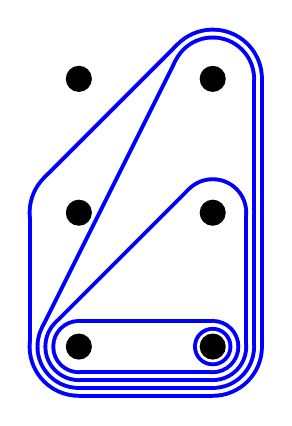
\begin{tikzpicture}
\node[fill] (1) at (0.0, 0.0) [circle] {};
\node[fill] (2) at (1.7, 0.0) [circle] {};
\node[fill] (3) at (0.0, -1.7) [circle] {};
\node[fill] (4) at (1.7, -1.7) [circle] {};
\node[fill] (5) at (0.0, -3.4) [circle] {};
\node[fill] (6) at (1.7, -3.4) [circle] {};
%23456
\begin{scope}[on background layer]
\fill[\tubecolor] (2) circle (\n + 9*\thickness);
\fill[\tubecolor] (3) circle (\n + 9*\thickness);
\fill[\tubecolor] (4) circle (\n + 9*\thickness);
\fill[\tubecolor] (5) circle (\n + 9*\thickness);
\fill[\tubecolor] (6) circle (\n + 9*\thickness);
\draw[\tubecolor] [line width = 2*(\n + 9*\thickness)] (2.center) -- (3.center);
\draw[\tubecolor] [line width = 2*(\n + 9*\thickness)] (2.center) -- (4.center);
\draw[\tubecolor] [line width = 2*(\n + 9*\thickness)] (2.center) -- (5.center);
\draw[\tubecolor] [line width = 2*(\n + 9*\thickness)] (3.center) -- (4.center);
\draw[\tubecolor] [line width = 2*(\n + 9*\thickness)] (3.center) -- (5.center);
\draw[\tubecolor] [line width = 2*(\n + 9*\thickness)] (3.center) -- (6.center);
\draw[\tubecolor] [line width = 2*(\n + 9*\thickness)] (4.center) -- (5.center);
\draw[\tubecolor] [line width = 2*(\n + 9*\thickness)] (4.center) -- (6.center);
\draw[\tubecolor] [line width = 2*(\n + 9*\thickness)] (5.center) -- (6.center);
\draw[white] [line width = 2*(\n + 8*\thickness)] (2.center) -- (3.center);
\draw[white] [line width = 2*(\n + 8*\thickness)] (2.center) -- (4.center);
\draw[white] [line width = 2*(\n + 8*\thickness)] (2.center) -- (5.center);
\draw[white] [line width = 2*(\n + 8*\thickness)] (3.center) -- (4.center);
\draw[white] [line width = 2*(\n + 8*\thickness)] (3.center) -- (5.center);
\draw[white] [line width = 2*(\n + 8*\thickness)] (3.center) -- (6.center);
\draw[white] [line width = 2*(\n + 8*\thickness)] (4.center) -- (5.center);
\draw[white] [line width = 2*(\n + 8*\thickness)] (4.center) -- (6.center);
\draw[white] [line width = 2*(\n + 8*\thickness)] (5.center) -- (6.center);
\fill[white] (2.center) -- (4.center) -- (3.center) -- (2.center);
\fill[white] (3.center) -- (5.center) -- (2.center) -- (3.center);
\fill[white] (2.center) -- (4.center) -- (5.center) -- (2.center);
\fill[white] (3.center) -- (5.center) -- (4.center) -- (3.center);
\fill[white] (4.center) -- (6.center) -- (3.center) -- (4.center);
\fill[white] (3.center) -- (5.center) -- (6.center) -- (3.center);
\fill[white] (4.center) -- (6.center) -- (5.center) -- (4.center);
\fill[white] (2) circle (\n + 8*\thickness);
\fill[white] (3) circle (\n + 8*\thickness);
\fill[white] (4) circle (\n + 8*\thickness);
\fill[white] (5) circle (\n + 8*\thickness);
\fill[white] (6) circle (\n + 8*\thickness);
\end{scope}
%2456
\begin{scope}[on background layer]
\fill[\tubecolor] (2) circle (\n + 7*\thickness);
\fill[\tubecolor] (4) circle (\n + 7*\thickness);
\fill[\tubecolor] (5) circle (\n + 7*\thickness);
\fill[\tubecolor] (6) circle (\n + 7*\thickness);
\draw[\tubecolor] [line width = 2*(\n + 7*\thickness)] (2.center) -- (4.center);
\draw[\tubecolor] [line width = 2*(\n + 7*\thickness)] (2.center) -- (5.center);
\draw[\tubecolor] [line width = 2*(\n + 7*\thickness)] (4.center) -- (5.center);
\draw[\tubecolor] [line width = 2*(\n + 7*\thickness)] (4.center) -- (6.center);
\draw[\tubecolor] [line width = 2*(\n + 7*\thickness)] (5.center) -- (6.center);
\draw[white] [line width = 2*(\n + 6*\thickness)] (2.center) -- (4.center);
\draw[white] [line width = 2*(\n + 6*\thickness)] (2.center) -- (5.center);
\draw[white] [line width = 2*(\n + 6*\thickness)] (4.center) -- (5.center);
\draw[white] [line width = 2*(\n + 6*\thickness)] (4.center) -- (6.center);
\draw[white] [line width = 2*(\n + 6*\thickness)] (5.center) -- (6.center);
\fill[white] (2.center) -- (4.center) -- (5.center) -- (2.center);
\fill[white] (4.center) -- (6.center) -- (5.center) -- (4.center);
\fill[white] (2) circle (\n + 6*\thickness);
\fill[white] (4) circle (\n + 6*\thickness);
\fill[white] (5) circle (\n + 6*\thickness);
\fill[white] (6) circle (\n + 6*\thickness);
\end{scope}
%456
\begin{scope}[on background layer]
\fill[\tubecolor] (4) circle (\n + 5*\thickness);
\fill[\tubecolor] (5) circle (\n + 5*\thickness);
\fill[\tubecolor] (6) circle (\n + 5*\thickness);
\draw[\tubecolor] [line width = 2*(\n + 5*\thickness)] (4.center) -- (5.center);
\draw[\tubecolor] [line width = 2*(\n + 5*\thickness)] (4.center) -- (6.center);
\draw[\tubecolor] [line width = 2*(\n + 5*\thickness)] (5.center) -- (6.center);
\draw[white] [line width = 2*(\n + 4*\thickness)] (4.center) -- (5.center);
\draw[white] [line width = 2*(\n + 4*\thickness)] (4.center) -- (6.center);
\draw[white] [line width = 2*(\n + 4*\thickness)] (5.center) -- (6.center);
\fill[white] (4.center) -- (6.center) -- (5.center) -- (4.center);
\fill[white] (4) circle (\n + 4*\thickness);
\fill[white] (5) circle (\n + 4*\thickness);
\fill[white] (6) circle (\n + 4*\thickness);
\end{scope}
%56
\begin{scope}[on background layer]
\fill[\tubecolor] (5) circle (\n + 3*\thickness);
\fill[\tubecolor] (6) circle (\n + 3*\thickness);
\draw[\tubecolor] [line width = 2*(\n + 3*\thickness)] (5.center) -- (6.center);
\draw[white] [line width = 2*(\n + 2*\thickness)] (5.center) -- (6.center);
\fill[white] (5) circle (\n + 2*\thickness);
\fill[white] (6) circle (\n + 2*\thickness);
\end{scope}
%6
\begin{scope}[on background layer]
\fill[\tubecolor] (6) circle (\n + 1*\thickness);
\fill[white] (6) circle (\n + 0*\thickness);
\end{scope}
\end{tikzpicture}
%652431
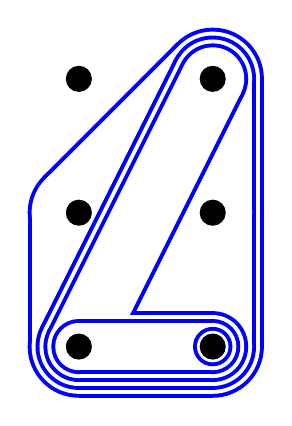
\begin{tikzpicture}
\node[fill] (1) at (0.0, 0.0) [circle] {};
\node[fill] (2) at (1.7, 0.0) [circle] {};
\node[fill] (3) at (0.0, -1.7) [circle] {};
\node[fill] (4) at (1.7, -1.7) [circle] {};
\node[fill] (5) at (0.0, -3.4) [circle] {};
\node[fill] (6) at (1.7, -3.4) [circle] {};
%23456
\begin{scope}[on background layer]
\fill[\tubecolor] (2) circle (\n + 9*\thickness);
\fill[\tubecolor] (3) circle (\n + 9*\thickness);
\fill[\tubecolor] (4) circle (\n + 9*\thickness);
\fill[\tubecolor] (5) circle (\n + 9*\thickness);
\fill[\tubecolor] (6) circle (\n + 9*\thickness);
\draw[\tubecolor] [line width = 2*(\n + 9*\thickness)] (2.center) -- (3.center);
\draw[\tubecolor] [line width = 2*(\n + 9*\thickness)] (2.center) -- (4.center);
\draw[\tubecolor] [line width = 2*(\n + 9*\thickness)] (2.center) -- (5.center);
\draw[\tubecolor] [line width = 2*(\n + 9*\thickness)] (3.center) -- (4.center);
\draw[\tubecolor] [line width = 2*(\n + 9*\thickness)] (3.center) -- (5.center);
\draw[\tubecolor] [line width = 2*(\n + 9*\thickness)] (3.center) -- (6.center);
\draw[\tubecolor] [line width = 2*(\n + 9*\thickness)] (4.center) -- (5.center);
\draw[\tubecolor] [line width = 2*(\n + 9*\thickness)] (4.center) -- (6.center);
\draw[\tubecolor] [line width = 2*(\n + 9*\thickness)] (5.center) -- (6.center);
\draw[white] [line width = 2*(\n + 8*\thickness)] (2.center) -- (3.center);
\draw[white] [line width = 2*(\n + 8*\thickness)] (2.center) -- (4.center);
\draw[white] [line width = 2*(\n + 8*\thickness)] (2.center) -- (5.center);
\draw[white] [line width = 2*(\n + 8*\thickness)] (3.center) -- (4.center);
\draw[white] [line width = 2*(\n + 8*\thickness)] (3.center) -- (5.center);
\draw[white] [line width = 2*(\n + 8*\thickness)] (3.center) -- (6.center);
\draw[white] [line width = 2*(\n + 8*\thickness)] (4.center) -- (5.center);
\draw[white] [line width = 2*(\n + 8*\thickness)] (4.center) -- (6.center);
\draw[white] [line width = 2*(\n + 8*\thickness)] (5.center) -- (6.center);
\fill[white] (2.center) -- (4.center) -- (3.center) -- (2.center);
\fill[white] (3.center) -- (5.center) -- (2.center) -- (3.center);
\fill[white] (2.center) -- (4.center) -- (5.center) -- (2.center);
\fill[white] (3.center) -- (5.center) -- (4.center) -- (3.center);
\fill[white] (4.center) -- (6.center) -- (3.center) -- (4.center);
\fill[white] (3.center) -- (5.center) -- (6.center) -- (3.center);
\fill[white] (4.center) -- (6.center) -- (5.center) -- (4.center);
\fill[white] (2) circle (\n + 8*\thickness);
\fill[white] (3) circle (\n + 8*\thickness);
\fill[white] (4) circle (\n + 8*\thickness);
\fill[white] (5) circle (\n + 8*\thickness);
\fill[white] (6) circle (\n + 8*\thickness);
\end{scope}
%2456
\begin{scope}[on background layer]
\fill[\tubecolor] (2) circle (\n + 7*\thickness);
\fill[\tubecolor] (4) circle (\n + 7*\thickness);
\fill[\tubecolor] (5) circle (\n + 7*\thickness);
\fill[\tubecolor] (6) circle (\n + 7*\thickness);
\draw[\tubecolor] [line width = 2*(\n + 7*\thickness)] (2.center) -- (4.center);
\draw[\tubecolor] [line width = 2*(\n + 7*\thickness)] (2.center) -- (5.center);
\draw[\tubecolor] [line width = 2*(\n + 7*\thickness)] (4.center) -- (5.center);
\draw[\tubecolor] [line width = 2*(\n + 7*\thickness)] (4.center) -- (6.center);
\draw[\tubecolor] [line width = 2*(\n + 7*\thickness)] (5.center) -- (6.center);
\draw[white] [line width = 2*(\n + 6*\thickness)] (2.center) -- (4.center);
\draw[white] [line width = 2*(\n + 6*\thickness)] (2.center) -- (5.center);
\draw[white] [line width = 2*(\n + 6*\thickness)] (4.center) -- (5.center);
\draw[white] [line width = 2*(\n + 6*\thickness)] (4.center) -- (6.center);
\draw[white] [line width = 2*(\n + 6*\thickness)] (5.center) -- (6.center);
\fill[white] (2.center) -- (4.center) -- (5.center) -- (2.center);
\fill[white] (4.center) -- (6.center) -- (5.center) -- (4.center);
\fill[white] (2) circle (\n + 6*\thickness);
\fill[white] (4) circle (\n + 6*\thickness);
\fill[white] (5) circle (\n + 6*\thickness);
\fill[white] (6) circle (\n + 6*\thickness);
\end{scope}
%256
\begin{scope}[on background layer]
\fill[\tubecolor] (2) circle (\n + 5*\thickness);
\fill[\tubecolor] (5) circle (\n + 5*\thickness);
\fill[\tubecolor] (6) circle (\n + 5*\thickness);
\draw[\tubecolor] [line width = 2*(\n + 5*\thickness)] (2.center) -- (5.center);
\draw[\tubecolor] [line width = 2*(\n + 5*\thickness)] (5.center) -- (6.center);
\draw[white] [line width = 2*(\n + 4*\thickness)] (2.center) -- (5.center);
\draw[white] [line width = 2*(\n + 4*\thickness)] (5.center) -- (6.center);
\fill[white] (2) circle (\n + 4*\thickness);
\fill[white] (5) circle (\n + 4*\thickness);
\fill[white] (6) circle (\n + 4*\thickness);
\end{scope}
%56
\begin{scope}[on background layer]
\fill[\tubecolor] (5) circle (\n + 3*\thickness);
\fill[\tubecolor] (6) circle (\n + 3*\thickness);
\draw[\tubecolor] [line width = 2*(\n + 3*\thickness)] (5.center) -- (6.center);
\draw[white] [line width = 2*(\n + 2*\thickness)] (5.center) -- (6.center);
\fill[white] (5) circle (\n + 2*\thickness);
\fill[white] (6) circle (\n + 2*\thickness);
\end{scope}
%6
\begin{scope}[on background layer]
\fill[\tubecolor] (6) circle (\n + 1*\thickness);
\fill[white] (6) circle (\n + 0*\thickness);
\end{scope}
\end{tikzpicture}


%652341
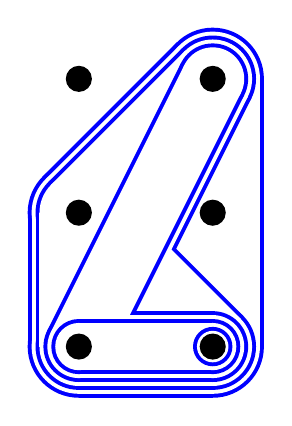
\begin{tikzpicture}
\node[fill] (1) at (0.0, 0.0) [circle] {};
\node[fill] (2) at (1.7, 0.0) [circle] {};
\node[fill] (3) at (0.0, -1.7) [circle] {};
\node[fill] (4) at (1.7, -1.7) [circle] {};
\node[fill] (5) at (0.0, -3.4) [circle] {};
\node[fill] (6) at (1.7, -3.4) [circle] {};
%23456
\begin{scope}[on background layer]
\fill[\tubecolor] (2) circle (\n + 9*\thickness);
\fill[\tubecolor] (3) circle (\n + 9*\thickness);
\fill[\tubecolor] (4) circle (\n + 9*\thickness);
\fill[\tubecolor] (5) circle (\n + 9*\thickness);
\fill[\tubecolor] (6) circle (\n + 9*\thickness);
\draw[\tubecolor] [line width = 2*(\n + 9*\thickness)] (2.center) -- (3.center);
\draw[\tubecolor] [line width = 2*(\n + 9*\thickness)] (2.center) -- (4.center);
\draw[\tubecolor] [line width = 2*(\n + 9*\thickness)] (2.center) -- (5.center);
\draw[\tubecolor] [line width = 2*(\n + 9*\thickness)] (3.center) -- (4.center);
\draw[\tubecolor] [line width = 2*(\n + 9*\thickness)] (3.center) -- (5.center);
\draw[\tubecolor] [line width = 2*(\n + 9*\thickness)] (3.center) -- (6.center);
\draw[\tubecolor] [line width = 2*(\n + 9*\thickness)] (4.center) -- (5.center);
\draw[\tubecolor] [line width = 2*(\n + 9*\thickness)] (4.center) -- (6.center);
\draw[\tubecolor] [line width = 2*(\n + 9*\thickness)] (5.center) -- (6.center);
\draw[white] [line width = 2*(\n + 8*\thickness)] (2.center) -- (3.center);
\draw[white] [line width = 2*(\n + 8*\thickness)] (2.center) -- (4.center);
\draw[white] [line width = 2*(\n + 8*\thickness)] (2.center) -- (5.center);
\draw[white] [line width = 2*(\n + 8*\thickness)] (3.center) -- (4.center);
\draw[white] [line width = 2*(\n + 8*\thickness)] (3.center) -- (5.center);
\draw[white] [line width = 2*(\n + 8*\thickness)] (3.center) -- (6.center);
\draw[white] [line width = 2*(\n + 8*\thickness)] (4.center) -- (5.center);
\draw[white] [line width = 2*(\n + 8*\thickness)] (4.center) -- (6.center);
\draw[white] [line width = 2*(\n + 8*\thickness)] (5.center) -- (6.center);
\fill[white] (2.center) -- (4.center) -- (3.center) -- (2.center);
\fill[white] (3.center) -- (5.center) -- (2.center) -- (3.center);
\fill[white] (2.center) -- (4.center) -- (5.center) -- (2.center);
\fill[white] (3.center) -- (5.center) -- (4.center) -- (3.center);
\fill[white] (4.center) -- (6.center) -- (3.center) -- (4.center);
\fill[white] (3.center) -- (5.center) -- (6.center) -- (3.center);
\fill[white] (4.center) -- (6.center) -- (5.center) -- (4.center);
\fill[white] (2) circle (\n + 8*\thickness);
\fill[white] (3) circle (\n + 8*\thickness);
\fill[white] (4) circle (\n + 8*\thickness);
\fill[white] (5) circle (\n + 8*\thickness);
\fill[white] (6) circle (\n + 8*\thickness);
\end{scope}
%2356
\begin{scope}[on background layer]
\fill[\tubecolor] (2) circle (\n + 7*\thickness);
\fill[\tubecolor] (3) circle (\n + 7*\thickness);
\fill[\tubecolor] (5) circle (\n + 7*\thickness);
\fill[\tubecolor] (6) circle (\n + 7*\thickness);
\draw[\tubecolor] [line width = 2*(\n + 7*\thickness)] (2.center) -- (3.center);
\draw[\tubecolor] [line width = 2*(\n + 7*\thickness)] (2.center) -- (5.center);
\draw[\tubecolor] [line width = 2*(\n + 7*\thickness)] (3.center) -- (5.center);
\draw[\tubecolor] [line width = 2*(\n + 7*\thickness)] (3.center) -- (6.center);
\draw[\tubecolor] [line width = 2*(\n + 7*\thickness)] (5.center) -- (6.center);
\draw[white] [line width = 2*(\n + 6*\thickness)] (2.center) -- (3.center);
\draw[white] [line width = 2*(\n + 6*\thickness)] (2.center) -- (5.center);
\draw[white] [line width = 2*(\n + 6*\thickness)] (3.center) -- (5.center);
\draw[white] [line width = 2*(\n + 6*\thickness)] (3.center) -- (6.center);
\draw[white] [line width = 2*(\n + 6*\thickness)] (5.center) -- (6.center);
\fill[white] (3.center) -- (5.center) -- (2.center) -- (3.center);
\fill[white] (3.center) -- (5.center) -- (6.center) -- (3.center);
\fill[white] (2) circle (\n + 6*\thickness);
\fill[white] (3) circle (\n + 6*\thickness);
\fill[white] (5) circle (\n + 6*\thickness);
\fill[white] (6) circle (\n + 6*\thickness);
\end{scope}
%256
\begin{scope}[on background layer]
\fill[\tubecolor] (2) circle (\n + 5*\thickness);
\fill[\tubecolor] (5) circle (\n + 5*\thickness);
\fill[\tubecolor] (6) circle (\n + 5*\thickness);
\draw[\tubecolor] [line width = 2*(\n + 5*\thickness)] (2.center) -- (5.center);
\draw[\tubecolor] [line width = 2*(\n + 5*\thickness)] (5.center) -- (6.center);
\draw[white] [line width = 2*(\n + 4*\thickness)] (2.center) -- (5.center);
\draw[white] [line width = 2*(\n + 4*\thickness)] (5.center) -- (6.center);
\fill[white] (2) circle (\n + 4*\thickness);
\fill[white] (5) circle (\n + 4*\thickness);
\fill[white] (6) circle (\n + 4*\thickness);
\end{scope}
%56
\begin{scope}[on background layer]
\fill[\tubecolor] (5) circle (\n + 3*\thickness);
\fill[\tubecolor] (6) circle (\n + 3*\thickness);
\draw[\tubecolor] [line width = 2*(\n + 3*\thickness)] (5.center) -- (6.center);
\draw[white] [line width = 2*(\n + 2*\thickness)] (5.center) -- (6.center);
\fill[white] (5) circle (\n + 2*\thickness);
\fill[white] (6) circle (\n + 2*\thickness);
\end{scope}
%6
\begin{scope}[on background layer]
\fill[\tubecolor] (6) circle (\n + 1*\thickness);
\fill[white] (6) circle (\n + 0*\thickness);
\end{scope}
\end{tikzpicture}
%562341
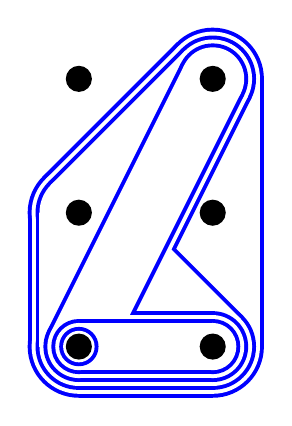
\begin{tikzpicture}
\node[fill] (1) at (0.0, 0.0) [circle] {};
\node[fill] (2) at (1.7, 0.0) [circle] {};
\node[fill] (3) at (0.0, -1.7) [circle] {};
\node[fill] (4) at (1.7, -1.7) [circle] {};
\node[fill] (5) at (0.0, -3.4) [circle] {};
\node[fill] (6) at (1.7, -3.4) [circle] {};
%23456
\begin{scope}[on background layer]
\fill[\tubecolor] (2) circle (\n + 9*\thickness);
\fill[\tubecolor] (3) circle (\n + 9*\thickness);
\fill[\tubecolor] (4) circle (\n + 9*\thickness);
\fill[\tubecolor] (5) circle (\n + 9*\thickness);
\fill[\tubecolor] (6) circle (\n + 9*\thickness);
\draw[\tubecolor] [line width = 2*(\n + 9*\thickness)] (2.center) -- (3.center);
\draw[\tubecolor] [line width = 2*(\n + 9*\thickness)] (2.center) -- (4.center);
\draw[\tubecolor] [line width = 2*(\n + 9*\thickness)] (2.center) -- (5.center);
\draw[\tubecolor] [line width = 2*(\n + 9*\thickness)] (3.center) -- (4.center);
\draw[\tubecolor] [line width = 2*(\n + 9*\thickness)] (3.center) -- (5.center);
\draw[\tubecolor] [line width = 2*(\n + 9*\thickness)] (3.center) -- (6.center);
\draw[\tubecolor] [line width = 2*(\n + 9*\thickness)] (4.center) -- (5.center);
\draw[\tubecolor] [line width = 2*(\n + 9*\thickness)] (4.center) -- (6.center);
\draw[\tubecolor] [line width = 2*(\n + 9*\thickness)] (5.center) -- (6.center);
\draw[white] [line width = 2*(\n + 8*\thickness)] (2.center) -- (3.center);
\draw[white] [line width = 2*(\n + 8*\thickness)] (2.center) -- (4.center);
\draw[white] [line width = 2*(\n + 8*\thickness)] (2.center) -- (5.center);
\draw[white] [line width = 2*(\n + 8*\thickness)] (3.center) -- (4.center);
\draw[white] [line width = 2*(\n + 8*\thickness)] (3.center) -- (5.center);
\draw[white] [line width = 2*(\n + 8*\thickness)] (3.center) -- (6.center);
\draw[white] [line width = 2*(\n + 8*\thickness)] (4.center) -- (5.center);
\draw[white] [line width = 2*(\n + 8*\thickness)] (4.center) -- (6.center);
\draw[white] [line width = 2*(\n + 8*\thickness)] (5.center) -- (6.center);
\fill[white] (2.center) -- (4.center) -- (3.center) -- (2.center);
\fill[white] (3.center) -- (5.center) -- (2.center) -- (3.center);
\fill[white] (2.center) -- (4.center) -- (5.center) -- (2.center);
\fill[white] (3.center) -- (5.center) -- (4.center) -- (3.center);
\fill[white] (4.center) -- (6.center) -- (3.center) -- (4.center);
\fill[white] (3.center) -- (5.center) -- (6.center) -- (3.center);
\fill[white] (4.center) -- (6.center) -- (5.center) -- (4.center);
\fill[white] (2) circle (\n + 8*\thickness);
\fill[white] (3) circle (\n + 8*\thickness);
\fill[white] (4) circle (\n + 8*\thickness);
\fill[white] (5) circle (\n + 8*\thickness);
\fill[white] (6) circle (\n + 8*\thickness);
\end{scope}
%2356
\begin{scope}[on background layer]
\fill[\tubecolor] (2) circle (\n + 7*\thickness);
\fill[\tubecolor] (3) circle (\n + 7*\thickness);
\fill[\tubecolor] (5) circle (\n + 7*\thickness);
\fill[\tubecolor] (6) circle (\n + 7*\thickness);
\draw[\tubecolor] [line width = 2*(\n + 7*\thickness)] (2.center) -- (3.center);
\draw[\tubecolor] [line width = 2*(\n + 7*\thickness)] (2.center) -- (5.center);
\draw[\tubecolor] [line width = 2*(\n + 7*\thickness)] (3.center) -- (5.center);
\draw[\tubecolor] [line width = 2*(\n + 7*\thickness)] (3.center) -- (6.center);
\draw[\tubecolor] [line width = 2*(\n + 7*\thickness)] (5.center) -- (6.center);
\draw[white] [line width = 2*(\n + 6*\thickness)] (2.center) -- (3.center);
\draw[white] [line width = 2*(\n + 6*\thickness)] (2.center) -- (5.center);
\draw[white] [line width = 2*(\n + 6*\thickness)] (3.center) -- (5.center);
\draw[white] [line width = 2*(\n + 6*\thickness)] (3.center) -- (6.center);
\draw[white] [line width = 2*(\n + 6*\thickness)] (5.center) -- (6.center);
\fill[white] (3.center) -- (5.center) -- (2.center) -- (3.center);
\fill[white] (3.center) -- (5.center) -- (6.center) -- (3.center);
\fill[white] (2) circle (\n + 6*\thickness);
\fill[white] (3) circle (\n + 6*\thickness);
\fill[white] (5) circle (\n + 6*\thickness);
\fill[white] (6) circle (\n + 6*\thickness);
\end{scope}
%256
\begin{scope}[on background layer]
\fill[\tubecolor] (2) circle (\n + 5*\thickness);
\fill[\tubecolor] (5) circle (\n + 5*\thickness);
\fill[\tubecolor] (6) circle (\n + 5*\thickness);
\draw[\tubecolor] [line width = 2*(\n + 5*\thickness)] (2.center) -- (5.center);
\draw[\tubecolor] [line width = 2*(\n + 5*\thickness)] (5.center) -- (6.center);
\draw[white] [line width = 2*(\n + 4*\thickness)] (2.center) -- (5.center);
\draw[white] [line width = 2*(\n + 4*\thickness)] (5.center) -- (6.center);
\fill[white] (2) circle (\n + 4*\thickness);
\fill[white] (5) circle (\n + 4*\thickness);
\fill[white] (6) circle (\n + 4*\thickness);
\end{scope}
%56
\begin{scope}[on background layer]
\fill[\tubecolor] (5) circle (\n + 3*\thickness);
\fill[\tubecolor] (6) circle (\n + 3*\thickness);
\draw[\tubecolor] [line width = 2*(\n + 3*\thickness)] (5.center) -- (6.center);
\draw[white] [line width = 2*(\n + 2*\thickness)] (5.center) -- (6.center);
\fill[white] (5) circle (\n + 2*\thickness);
\fill[white] (6) circle (\n + 2*\thickness);
\end{scope}
%5
\begin{scope}[on background layer]
\fill[\tubecolor] (5) circle (\n + 1*\thickness);
\fill[white] (5) circle (\n + 0*\thickness);
\end{scope}
\end{tikzpicture}
%526341
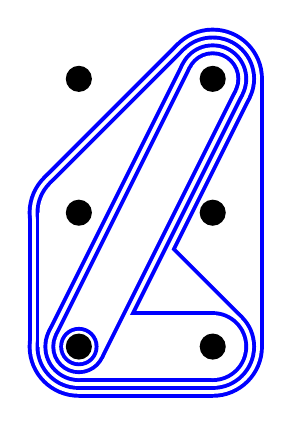
\begin{tikzpicture}
\node[fill] (1) at (0.0, 0.0) [circle] {};
\node[fill] (2) at (1.7, 0.0) [circle] {};
\node[fill] (3) at (0.0, -1.7) [circle] {};
\node[fill] (4) at (1.7, -1.7) [circle] {};
\node[fill] (5) at (0.0, -3.4) [circle] {};
\node[fill] (6) at (1.7, -3.4) [circle] {};
%23456
\begin{scope}[on background layer]
\fill[\tubecolor] (2) circle (\n + 9*\thickness);
\fill[\tubecolor] (3) circle (\n + 9*\thickness);
\fill[\tubecolor] (4) circle (\n + 9*\thickness);
\fill[\tubecolor] (5) circle (\n + 9*\thickness);
\fill[\tubecolor] (6) circle (\n + 9*\thickness);
\draw[\tubecolor] [line width = 2*(\n + 9*\thickness)] (2.center) -- (3.center);
\draw[\tubecolor] [line width = 2*(\n + 9*\thickness)] (2.center) -- (4.center);
\draw[\tubecolor] [line width = 2*(\n + 9*\thickness)] (2.center) -- (5.center);
\draw[\tubecolor] [line width = 2*(\n + 9*\thickness)] (3.center) -- (4.center);
\draw[\tubecolor] [line width = 2*(\n + 9*\thickness)] (3.center) -- (5.center);
\draw[\tubecolor] [line width = 2*(\n + 9*\thickness)] (3.center) -- (6.center);
\draw[\tubecolor] [line width = 2*(\n + 9*\thickness)] (4.center) -- (5.center);
\draw[\tubecolor] [line width = 2*(\n + 9*\thickness)] (4.center) -- (6.center);
\draw[\tubecolor] [line width = 2*(\n + 9*\thickness)] (5.center) -- (6.center);
\draw[white] [line width = 2*(\n + 8*\thickness)] (2.center) -- (3.center);
\draw[white] [line width = 2*(\n + 8*\thickness)] (2.center) -- (4.center);
\draw[white] [line width = 2*(\n + 8*\thickness)] (2.center) -- (5.center);
\draw[white] [line width = 2*(\n + 8*\thickness)] (3.center) -- (4.center);
\draw[white] [line width = 2*(\n + 8*\thickness)] (3.center) -- (5.center);
\draw[white] [line width = 2*(\n + 8*\thickness)] (3.center) -- (6.center);
\draw[white] [line width = 2*(\n + 8*\thickness)] (4.center) -- (5.center);
\draw[white] [line width = 2*(\n + 8*\thickness)] (4.center) -- (6.center);
\draw[white] [line width = 2*(\n + 8*\thickness)] (5.center) -- (6.center);
\fill[white] (2.center) -- (4.center) -- (3.center) -- (2.center);
\fill[white] (3.center) -- (5.center) -- (2.center) -- (3.center);
\fill[white] (2.center) -- (4.center) -- (5.center) -- (2.center);
\fill[white] (3.center) -- (5.center) -- (4.center) -- (3.center);
\fill[white] (4.center) -- (6.center) -- (3.center) -- (4.center);
\fill[white] (3.center) -- (5.center) -- (6.center) -- (3.center);
\fill[white] (4.center) -- (6.center) -- (5.center) -- (4.center);
\fill[white] (2) circle (\n + 8*\thickness);
\fill[white] (3) circle (\n + 8*\thickness);
\fill[white] (4) circle (\n + 8*\thickness);
\fill[white] (5) circle (\n + 8*\thickness);
\fill[white] (6) circle (\n + 8*\thickness);
\end{scope}
%2356
\begin{scope}[on background layer]
\fill[\tubecolor] (2) circle (\n + 7*\thickness);
\fill[\tubecolor] (3) circle (\n + 7*\thickness);
\fill[\tubecolor] (5) circle (\n + 7*\thickness);
\fill[\tubecolor] (6) circle (\n + 7*\thickness);
\draw[\tubecolor] [line width = 2*(\n + 7*\thickness)] (2.center) -- (3.center);
\draw[\tubecolor] [line width = 2*(\n + 7*\thickness)] (2.center) -- (5.center);
\draw[\tubecolor] [line width = 2*(\n + 7*\thickness)] (3.center) -- (5.center);
\draw[\tubecolor] [line width = 2*(\n + 7*\thickness)] (3.center) -- (6.center);
\draw[\tubecolor] [line width = 2*(\n + 7*\thickness)] (5.center) -- (6.center);
\draw[white] [line width = 2*(\n + 6*\thickness)] (2.center) -- (3.center);
\draw[white] [line width = 2*(\n + 6*\thickness)] (2.center) -- (5.center);
\draw[white] [line width = 2*(\n + 6*\thickness)] (3.center) -- (5.center);
\draw[white] [line width = 2*(\n + 6*\thickness)] (3.center) -- (6.center);
\draw[white] [line width = 2*(\n + 6*\thickness)] (5.center) -- (6.center);
\fill[white] (3.center) -- (5.center) -- (2.center) -- (3.center);
\fill[white] (3.center) -- (5.center) -- (6.center) -- (3.center);
\fill[white] (2) circle (\n + 6*\thickness);
\fill[white] (3) circle (\n + 6*\thickness);
\fill[white] (5) circle (\n + 6*\thickness);
\fill[white] (6) circle (\n + 6*\thickness);
\end{scope}
%256
\begin{scope}[on background layer]
\fill[\tubecolor] (2) circle (\n + 5*\thickness);
\fill[\tubecolor] (5) circle (\n + 5*\thickness);
\fill[\tubecolor] (6) circle (\n + 5*\thickness);
\draw[\tubecolor] [line width = 2*(\n + 5*\thickness)] (2.center) -- (5.center);
\draw[\tubecolor] [line width = 2*(\n + 5*\thickness)] (5.center) -- (6.center);
\draw[white] [line width = 2*(\n + 4*\thickness)] (2.center) -- (5.center);
\draw[white] [line width = 2*(\n + 4*\thickness)] (5.center) -- (6.center);
\fill[white] (2) circle (\n + 4*\thickness);
\fill[white] (5) circle (\n + 4*\thickness);
\fill[white] (6) circle (\n + 4*\thickness);
\end{scope}
%25
\begin{scope}[on background layer]
\fill[\tubecolor] (2) circle (\n + 3*\thickness);
\fill[\tubecolor] (5) circle (\n + 3*\thickness);
\draw[\tubecolor] [line width = 2*(\n + 3*\thickness)] (2.center) -- (5.center);
\draw[white] [line width = 2*(\n + 2*\thickness)] (2.center) -- (5.center);
\fill[white] (2) circle (\n + 2*\thickness);
\fill[white] (5) circle (\n + 2*\thickness);
\end{scope}
%5
\begin{scope}[on background layer]
\fill[\tubecolor] (5) circle (\n + 1*\thickness);
\fill[white] (5) circle (\n + 0*\thickness);
\end{scope}
\end{tikzpicture}
%523641
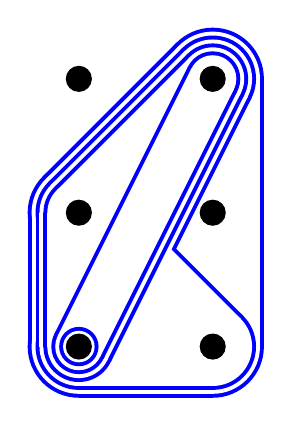
\begin{tikzpicture}
\node[fill] (1) at (0.0, 0.0) [circle] {};
\node[fill] (2) at (1.7, 0.0) [circle] {};
\node[fill] (3) at (0.0, -1.7) [circle] {};
\node[fill] (4) at (1.7, -1.7) [circle] {};
\node[fill] (5) at (0.0, -3.4) [circle] {};
\node[fill] (6) at (1.7, -3.4) [circle] {};
%23456
\begin{scope}[on background layer]
\fill[\tubecolor] (2) circle (\n + 9*\thickness);
\fill[\tubecolor] (3) circle (\n + 9*\thickness);
\fill[\tubecolor] (4) circle (\n + 9*\thickness);
\fill[\tubecolor] (5) circle (\n + 9*\thickness);
\fill[\tubecolor] (6) circle (\n + 9*\thickness);
\draw[\tubecolor] [line width = 2*(\n + 9*\thickness)] (2.center) -- (3.center);
\draw[\tubecolor] [line width = 2*(\n + 9*\thickness)] (2.center) -- (4.center);
\draw[\tubecolor] [line width = 2*(\n + 9*\thickness)] (2.center) -- (5.center);
\draw[\tubecolor] [line width = 2*(\n + 9*\thickness)] (3.center) -- (4.center);
\draw[\tubecolor] [line width = 2*(\n + 9*\thickness)] (3.center) -- (5.center);
\draw[\tubecolor] [line width = 2*(\n + 9*\thickness)] (3.center) -- (6.center);
\draw[\tubecolor] [line width = 2*(\n + 9*\thickness)] (4.center) -- (5.center);
\draw[\tubecolor] [line width = 2*(\n + 9*\thickness)] (4.center) -- (6.center);
\draw[\tubecolor] [line width = 2*(\n + 9*\thickness)] (5.center) -- (6.center);
\draw[white] [line width = 2*(\n + 8*\thickness)] (2.center) -- (3.center);
\draw[white] [line width = 2*(\n + 8*\thickness)] (2.center) -- (4.center);
\draw[white] [line width = 2*(\n + 8*\thickness)] (2.center) -- (5.center);
\draw[white] [line width = 2*(\n + 8*\thickness)] (3.center) -- (4.center);
\draw[white] [line width = 2*(\n + 8*\thickness)] (3.center) -- (5.center);
\draw[white] [line width = 2*(\n + 8*\thickness)] (3.center) -- (6.center);
\draw[white] [line width = 2*(\n + 8*\thickness)] (4.center) -- (5.center);
\draw[white] [line width = 2*(\n + 8*\thickness)] (4.center) -- (6.center);
\draw[white] [line width = 2*(\n + 8*\thickness)] (5.center) -- (6.center);
\fill[white] (2.center) -- (4.center) -- (3.center) -- (2.center);
\fill[white] (3.center) -- (5.center) -- (2.center) -- (3.center);
\fill[white] (2.center) -- (4.center) -- (5.center) -- (2.center);
\fill[white] (3.center) -- (5.center) -- (4.center) -- (3.center);
\fill[white] (4.center) -- (6.center) -- (3.center) -- (4.center);
\fill[white] (3.center) -- (5.center) -- (6.center) -- (3.center);
\fill[white] (4.center) -- (6.center) -- (5.center) -- (4.center);
\fill[white] (2) circle (\n + 8*\thickness);
\fill[white] (3) circle (\n + 8*\thickness);
\fill[white] (4) circle (\n + 8*\thickness);
\fill[white] (5) circle (\n + 8*\thickness);
\fill[white] (6) circle (\n + 8*\thickness);
\end{scope}
%2356
\begin{scope}[on background layer]
\fill[\tubecolor] (2) circle (\n + 7*\thickness);
\fill[\tubecolor] (3) circle (\n + 7*\thickness);
\fill[\tubecolor] (5) circle (\n + 7*\thickness);
\fill[\tubecolor] (6) circle (\n + 7*\thickness);
\draw[\tubecolor] [line width = 2*(\n + 7*\thickness)] (2.center) -- (3.center);
\draw[\tubecolor] [line width = 2*(\n + 7*\thickness)] (2.center) -- (5.center);
\draw[\tubecolor] [line width = 2*(\n + 7*\thickness)] (3.center) -- (5.center);
\draw[\tubecolor] [line width = 2*(\n + 7*\thickness)] (3.center) -- (6.center);
\draw[\tubecolor] [line width = 2*(\n + 7*\thickness)] (5.center) -- (6.center);
\draw[white] [line width = 2*(\n + 6*\thickness)] (2.center) -- (3.center);
\draw[white] [line width = 2*(\n + 6*\thickness)] (2.center) -- (5.center);
\draw[white] [line width = 2*(\n + 6*\thickness)] (3.center) -- (5.center);
\draw[white] [line width = 2*(\n + 6*\thickness)] (3.center) -- (6.center);
\draw[white] [line width = 2*(\n + 6*\thickness)] (5.center) -- (6.center);
\fill[white] (3.center) -- (5.center) -- (2.center) -- (3.center);
\fill[white] (3.center) -- (5.center) -- (6.center) -- (3.center);
\fill[white] (2) circle (\n + 6*\thickness);
\fill[white] (3) circle (\n + 6*\thickness);
\fill[white] (5) circle (\n + 6*\thickness);
\fill[white] (6) circle (\n + 6*\thickness);
\end{scope}
%235
\begin{scope}[on background layer]
\fill[\tubecolor] (2) circle (\n + 5*\thickness);
\fill[\tubecolor] (3) circle (\n + 5*\thickness);
\fill[\tubecolor] (5) circle (\n + 5*\thickness);
\draw[\tubecolor] [line width = 2*(\n + 5*\thickness)] (2.center) -- (3.center);
\draw[\tubecolor] [line width = 2*(\n + 5*\thickness)] (2.center) -- (5.center);
\draw[\tubecolor] [line width = 2*(\n + 5*\thickness)] (3.center) -- (5.center);
\draw[white] [line width = 2*(\n + 4*\thickness)] (2.center) -- (3.center);
\draw[white] [line width = 2*(\n + 4*\thickness)] (2.center) -- (5.center);
\draw[white] [line width = 2*(\n + 4*\thickness)] (3.center) -- (5.center);
\fill[white] (3.center) -- (5.center) -- (2.center) -- (3.center);
\fill[white] (2) circle (\n + 4*\thickness);
\fill[white] (3) circle (\n + 4*\thickness);
\fill[white] (5) circle (\n + 4*\thickness);
\end{scope}
%25
\begin{scope}[on background layer]
\fill[\tubecolor] (2) circle (\n + 3*\thickness);
\fill[\tubecolor] (5) circle (\n + 3*\thickness);
\draw[\tubecolor] [line width = 2*(\n + 3*\thickness)] (2.center) -- (5.center);
\draw[white] [line width = 2*(\n + 2*\thickness)] (2.center) -- (5.center);
\fill[white] (2) circle (\n + 2*\thickness);
\fill[white] (5) circle (\n + 2*\thickness);
\end{scope}
%5
\begin{scope}[on background layer]
\fill[\tubecolor] (5) circle (\n + 1*\thickness);
\fill[white] (5) circle (\n + 0*\thickness);
\end{scope}
\end{tikzpicture}
%523461
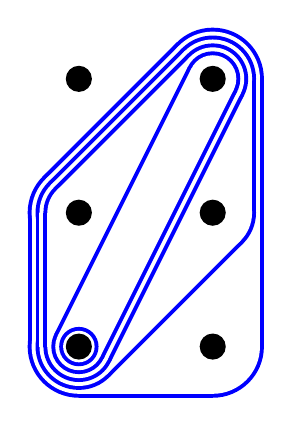
\begin{tikzpicture}
\node[fill] (1) at (0.0, 0.0) [circle] {};
\node[fill] (2) at (1.7, 0.0) [circle] {};
\node[fill] (3) at (0.0, -1.7) [circle] {};
\node[fill] (4) at (1.7, -1.7) [circle] {};
\node[fill] (5) at (0.0, -3.4) [circle] {};
\node[fill] (6) at (1.7, -3.4) [circle] {};
%23456
\begin{scope}[on background layer]
\fill[\tubecolor] (2) circle (\n + 9*\thickness);
\fill[\tubecolor] (3) circle (\n + 9*\thickness);
\fill[\tubecolor] (4) circle (\n + 9*\thickness);
\fill[\tubecolor] (5) circle (\n + 9*\thickness);
\fill[\tubecolor] (6) circle (\n + 9*\thickness);
\draw[\tubecolor] [line width = 2*(\n + 9*\thickness)] (2.center) -- (3.center);
\draw[\tubecolor] [line width = 2*(\n + 9*\thickness)] (2.center) -- (4.center);
\draw[\tubecolor] [line width = 2*(\n + 9*\thickness)] (2.center) -- (5.center);
\draw[\tubecolor] [line width = 2*(\n + 9*\thickness)] (3.center) -- (4.center);
\draw[\tubecolor] [line width = 2*(\n + 9*\thickness)] (3.center) -- (5.center);
\draw[\tubecolor] [line width = 2*(\n + 9*\thickness)] (3.center) -- (6.center);
\draw[\tubecolor] [line width = 2*(\n + 9*\thickness)] (4.center) -- (5.center);
\draw[\tubecolor] [line width = 2*(\n + 9*\thickness)] (4.center) -- (6.center);
\draw[\tubecolor] [line width = 2*(\n + 9*\thickness)] (5.center) -- (6.center);
\draw[white] [line width = 2*(\n + 8*\thickness)] (2.center) -- (3.center);
\draw[white] [line width = 2*(\n + 8*\thickness)] (2.center) -- (4.center);
\draw[white] [line width = 2*(\n + 8*\thickness)] (2.center) -- (5.center);
\draw[white] [line width = 2*(\n + 8*\thickness)] (3.center) -- (4.center);
\draw[white] [line width = 2*(\n + 8*\thickness)] (3.center) -- (5.center);
\draw[white] [line width = 2*(\n + 8*\thickness)] (3.center) -- (6.center);
\draw[white] [line width = 2*(\n + 8*\thickness)] (4.center) -- (5.center);
\draw[white] [line width = 2*(\n + 8*\thickness)] (4.center) -- (6.center);
\draw[white] [line width = 2*(\n + 8*\thickness)] (5.center) -- (6.center);
\fill[white] (2.center) -- (4.center) -- (3.center) -- (2.center);
\fill[white] (3.center) -- (5.center) -- (2.center) -- (3.center);
\fill[white] (2.center) -- (4.center) -- (5.center) -- (2.center);
\fill[white] (3.center) -- (5.center) -- (4.center) -- (3.center);
\fill[white] (4.center) -- (6.center) -- (3.center) -- (4.center);
\fill[white] (3.center) -- (5.center) -- (6.center) -- (3.center);
\fill[white] (4.center) -- (6.center) -- (5.center) -- (4.center);
\fill[white] (2) circle (\n + 8*\thickness);
\fill[white] (3) circle (\n + 8*\thickness);
\fill[white] (4) circle (\n + 8*\thickness);
\fill[white] (5) circle (\n + 8*\thickness);
\fill[white] (6) circle (\n + 8*\thickness);
\end{scope}
%2345
\begin{scope}[on background layer]
\fill[\tubecolor] (2) circle (\n + 7*\thickness);
\fill[\tubecolor] (3) circle (\n + 7*\thickness);
\fill[\tubecolor] (4) circle (\n + 7*\thickness);
\fill[\tubecolor] (5) circle (\n + 7*\thickness);
\draw[\tubecolor] [line width = 2*(\n + 7*\thickness)] (2.center) -- (3.center);
\draw[\tubecolor] [line width = 2*(\n + 7*\thickness)] (2.center) -- (4.center);
\draw[\tubecolor] [line width = 2*(\n + 7*\thickness)] (2.center) -- (5.center);
\draw[\tubecolor] [line width = 2*(\n + 7*\thickness)] (3.center) -- (4.center);
\draw[\tubecolor] [line width = 2*(\n + 7*\thickness)] (3.center) -- (5.center);
\draw[\tubecolor] [line width = 2*(\n + 7*\thickness)] (4.center) -- (5.center);
\draw[white] [line width = 2*(\n + 6*\thickness)] (2.center) -- (3.center);
\draw[white] [line width = 2*(\n + 6*\thickness)] (2.center) -- (4.center);
\draw[white] [line width = 2*(\n + 6*\thickness)] (2.center) -- (5.center);
\draw[white] [line width = 2*(\n + 6*\thickness)] (3.center) -- (4.center);
\draw[white] [line width = 2*(\n + 6*\thickness)] (3.center) -- (5.center);
\draw[white] [line width = 2*(\n + 6*\thickness)] (4.center) -- (5.center);
\fill[white] (2.center) -- (4.center) -- (3.center) -- (2.center);
\fill[white] (3.center) -- (5.center) -- (2.center) -- (3.center);
\fill[white] (2.center) -- (4.center) -- (5.center) -- (2.center);
\fill[white] (3.center) -- (5.center) -- (4.center) -- (3.center);
\fill[white] (2) circle (\n + 6*\thickness);
\fill[white] (3) circle (\n + 6*\thickness);
\fill[white] (4) circle (\n + 6*\thickness);
\fill[white] (5) circle (\n + 6*\thickness);
\end{scope}
%235
\begin{scope}[on background layer]
\fill[\tubecolor] (2) circle (\n + 5*\thickness);
\fill[\tubecolor] (3) circle (\n + 5*\thickness);
\fill[\tubecolor] (5) circle (\n + 5*\thickness);
\draw[\tubecolor] [line width = 2*(\n + 5*\thickness)] (2.center) -- (3.center);
\draw[\tubecolor] [line width = 2*(\n + 5*\thickness)] (2.center) -- (5.center);
\draw[\tubecolor] [line width = 2*(\n + 5*\thickness)] (3.center) -- (5.center);
\draw[white] [line width = 2*(\n + 4*\thickness)] (2.center) -- (3.center);
\draw[white] [line width = 2*(\n + 4*\thickness)] (2.center) -- (5.center);
\draw[white] [line width = 2*(\n + 4*\thickness)] (3.center) -- (5.center);
\fill[white] (3.center) -- (5.center) -- (2.center) -- (3.center);
\fill[white] (2) circle (\n + 4*\thickness);
\fill[white] (3) circle (\n + 4*\thickness);
\fill[white] (5) circle (\n + 4*\thickness);
\end{scope}
%25
\begin{scope}[on background layer]
\fill[\tubecolor] (2) circle (\n + 3*\thickness);
\fill[\tubecolor] (5) circle (\n + 3*\thickness);
\draw[\tubecolor] [line width = 2*(\n + 3*\thickness)] (2.center) -- (5.center);
\draw[white] [line width = 2*(\n + 2*\thickness)] (2.center) -- (5.center);
\fill[white] (2) circle (\n + 2*\thickness);
\fill[white] (5) circle (\n + 2*\thickness);
\end{scope}
%5
\begin{scope}[on background layer]
\fill[\tubecolor] (5) circle (\n + 1*\thickness);
\fill[white] (5) circle (\n + 0*\thickness);
\end{scope}
\end{tikzpicture}
%524361
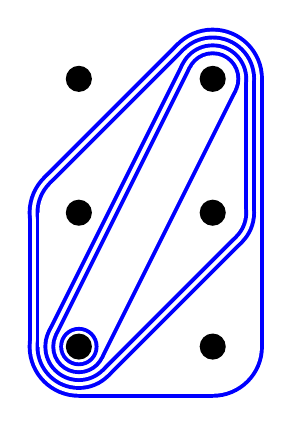
\begin{tikzpicture}
\node[fill] (1) at (0.0, 0.0) [circle] {};
\node[fill] (2) at (1.7, 0.0) [circle] {};
\node[fill] (3) at (0.0, -1.7) [circle] {};
\node[fill] (4) at (1.7, -1.7) [circle] {};
\node[fill] (5) at (0.0, -3.4) [circle] {};
\node[fill] (6) at (1.7, -3.4) [circle] {};
%23456
\begin{scope}[on background layer]
\fill[\tubecolor] (2) circle (\n + 9*\thickness);
\fill[\tubecolor] (3) circle (\n + 9*\thickness);
\fill[\tubecolor] (4) circle (\n + 9*\thickness);
\fill[\tubecolor] (5) circle (\n + 9*\thickness);
\fill[\tubecolor] (6) circle (\n + 9*\thickness);
\draw[\tubecolor] [line width = 2*(\n + 9*\thickness)] (2.center) -- (3.center);
\draw[\tubecolor] [line width = 2*(\n + 9*\thickness)] (2.center) -- (4.center);
\draw[\tubecolor] [line width = 2*(\n + 9*\thickness)] (2.center) -- (5.center);
\draw[\tubecolor] [line width = 2*(\n + 9*\thickness)] (3.center) -- (4.center);
\draw[\tubecolor] [line width = 2*(\n + 9*\thickness)] (3.center) -- (5.center);
\draw[\tubecolor] [line width = 2*(\n + 9*\thickness)] (3.center) -- (6.center);
\draw[\tubecolor] [line width = 2*(\n + 9*\thickness)] (4.center) -- (5.center);
\draw[\tubecolor] [line width = 2*(\n + 9*\thickness)] (4.center) -- (6.center);
\draw[\tubecolor] [line width = 2*(\n + 9*\thickness)] (5.center) -- (6.center);
\draw[white] [line width = 2*(\n + 8*\thickness)] (2.center) -- (3.center);
\draw[white] [line width = 2*(\n + 8*\thickness)] (2.center) -- (4.center);
\draw[white] [line width = 2*(\n + 8*\thickness)] (2.center) -- (5.center);
\draw[white] [line width = 2*(\n + 8*\thickness)] (3.center) -- (4.center);
\draw[white] [line width = 2*(\n + 8*\thickness)] (3.center) -- (5.center);
\draw[white] [line width = 2*(\n + 8*\thickness)] (3.center) -- (6.center);
\draw[white] [line width = 2*(\n + 8*\thickness)] (4.center) -- (5.center);
\draw[white] [line width = 2*(\n + 8*\thickness)] (4.center) -- (6.center);
\draw[white] [line width = 2*(\n + 8*\thickness)] (5.center) -- (6.center);
\fill[white] (2.center) -- (4.center) -- (3.center) -- (2.center);
\fill[white] (3.center) -- (5.center) -- (2.center) -- (3.center);
\fill[white] (2.center) -- (4.center) -- (5.center) -- (2.center);
\fill[white] (3.center) -- (5.center) -- (4.center) -- (3.center);
\fill[white] (4.center) -- (6.center) -- (3.center) -- (4.center);
\fill[white] (3.center) -- (5.center) -- (6.center) -- (3.center);
\fill[white] (4.center) -- (6.center) -- (5.center) -- (4.center);
\fill[white] (2) circle (\n + 8*\thickness);
\fill[white] (3) circle (\n + 8*\thickness);
\fill[white] (4) circle (\n + 8*\thickness);
\fill[white] (5) circle (\n + 8*\thickness);
\fill[white] (6) circle (\n + 8*\thickness);
\end{scope}
%2345
\begin{scope}[on background layer]
\fill[\tubecolor] (2) circle (\n + 7*\thickness);
\fill[\tubecolor] (3) circle (\n + 7*\thickness);
\fill[\tubecolor] (4) circle (\n + 7*\thickness);
\fill[\tubecolor] (5) circle (\n + 7*\thickness);
\draw[\tubecolor] [line width = 2*(\n + 7*\thickness)] (2.center) -- (3.center);
\draw[\tubecolor] [line width = 2*(\n + 7*\thickness)] (2.center) -- (4.center);
\draw[\tubecolor] [line width = 2*(\n + 7*\thickness)] (2.center) -- (5.center);
\draw[\tubecolor] [line width = 2*(\n + 7*\thickness)] (3.center) -- (4.center);
\draw[\tubecolor] [line width = 2*(\n + 7*\thickness)] (3.center) -- (5.center);
\draw[\tubecolor] [line width = 2*(\n + 7*\thickness)] (4.center) -- (5.center);
\draw[white] [line width = 2*(\n + 6*\thickness)] (2.center) -- (3.center);
\draw[white] [line width = 2*(\n + 6*\thickness)] (2.center) -- (4.center);
\draw[white] [line width = 2*(\n + 6*\thickness)] (2.center) -- (5.center);
\draw[white] [line width = 2*(\n + 6*\thickness)] (3.center) -- (4.center);
\draw[white] [line width = 2*(\n + 6*\thickness)] (3.center) -- (5.center);
\draw[white] [line width = 2*(\n + 6*\thickness)] (4.center) -- (5.center);
\fill[white] (2.center) -- (4.center) -- (3.center) -- (2.center);
\fill[white] (3.center) -- (5.center) -- (2.center) -- (3.center);
\fill[white] (2.center) -- (4.center) -- (5.center) -- (2.center);
\fill[white] (3.center) -- (5.center) -- (4.center) -- (3.center);
\fill[white] (2) circle (\n + 6*\thickness);
\fill[white] (3) circle (\n + 6*\thickness);
\fill[white] (4) circle (\n + 6*\thickness);
\fill[white] (5) circle (\n + 6*\thickness);
\end{scope}
%245
\begin{scope}[on background layer]
\fill[\tubecolor] (2) circle (\n + 5*\thickness);
\fill[\tubecolor] (4) circle (\n + 5*\thickness);
\fill[\tubecolor] (5) circle (\n + 5*\thickness);
\draw[\tubecolor] [line width = 2*(\n + 5*\thickness)] (2.center) -- (4.center);
\draw[\tubecolor] [line width = 2*(\n + 5*\thickness)] (2.center) -- (5.center);
\draw[\tubecolor] [line width = 2*(\n + 5*\thickness)] (4.center) -- (5.center);
\draw[white] [line width = 2*(\n + 4*\thickness)] (2.center) -- (4.center);
\draw[white] [line width = 2*(\n + 4*\thickness)] (2.center) -- (5.center);
\draw[white] [line width = 2*(\n + 4*\thickness)] (4.center) -- (5.center);
\fill[white] (2.center) -- (4.center) -- (5.center) -- (2.center);
\fill[white] (2) circle (\n + 4*\thickness);
\fill[white] (4) circle (\n + 4*\thickness);
\fill[white] (5) circle (\n + 4*\thickness);
\end{scope}
%25
\begin{scope}[on background layer]
\fill[\tubecolor] (2) circle (\n + 3*\thickness);
\fill[\tubecolor] (5) circle (\n + 3*\thickness);
\draw[\tubecolor] [line width = 2*(\n + 3*\thickness)] (2.center) -- (5.center);
\draw[white] [line width = 2*(\n + 2*\thickness)] (2.center) -- (5.center);
\fill[white] (2) circle (\n + 2*\thickness);
\fill[white] (5) circle (\n + 2*\thickness);
\end{scope}
%5
\begin{scope}[on background layer]
\fill[\tubecolor] (5) circle (\n + 1*\thickness);
\fill[white] (5) circle (\n + 0*\thickness);
\end{scope}
\end{tikzpicture}
%542361
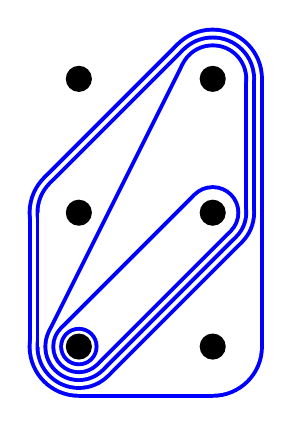
\begin{tikzpicture}
\node[fill] (1) at (0.0, 0.0) [circle] {};
\node[fill] (2) at (1.7, 0.0) [circle] {};
\node[fill] (3) at (0.0, -1.7) [circle] {};
\node[fill] (4) at (1.7, -1.7) [circle] {};
\node[fill] (5) at (0.0, -3.4) [circle] {};
\node[fill] (6) at (1.7, -3.4) [circle] {};
%23456
\begin{scope}[on background layer]
\fill[\tubecolor] (2) circle (\n + 9*\thickness);
\fill[\tubecolor] (3) circle (\n + 9*\thickness);
\fill[\tubecolor] (4) circle (\n + 9*\thickness);
\fill[\tubecolor] (5) circle (\n + 9*\thickness);
\fill[\tubecolor] (6) circle (\n + 9*\thickness);
\draw[\tubecolor] [line width = 2*(\n + 9*\thickness)] (2.center) -- (3.center);
\draw[\tubecolor] [line width = 2*(\n + 9*\thickness)] (2.center) -- (4.center);
\draw[\tubecolor] [line width = 2*(\n + 9*\thickness)] (2.center) -- (5.center);
\draw[\tubecolor] [line width = 2*(\n + 9*\thickness)] (3.center) -- (4.center);
\draw[\tubecolor] [line width = 2*(\n + 9*\thickness)] (3.center) -- (5.center);
\draw[\tubecolor] [line width = 2*(\n + 9*\thickness)] (3.center) -- (6.center);
\draw[\tubecolor] [line width = 2*(\n + 9*\thickness)] (4.center) -- (5.center);
\draw[\tubecolor] [line width = 2*(\n + 9*\thickness)] (4.center) -- (6.center);
\draw[\tubecolor] [line width = 2*(\n + 9*\thickness)] (5.center) -- (6.center);
\draw[white] [line width = 2*(\n + 8*\thickness)] (2.center) -- (3.center);
\draw[white] [line width = 2*(\n + 8*\thickness)] (2.center) -- (4.center);
\draw[white] [line width = 2*(\n + 8*\thickness)] (2.center) -- (5.center);
\draw[white] [line width = 2*(\n + 8*\thickness)] (3.center) -- (4.center);
\draw[white] [line width = 2*(\n + 8*\thickness)] (3.center) -- (5.center);
\draw[white] [line width = 2*(\n + 8*\thickness)] (3.center) -- (6.center);
\draw[white] [line width = 2*(\n + 8*\thickness)] (4.center) -- (5.center);
\draw[white] [line width = 2*(\n + 8*\thickness)] (4.center) -- (6.center);
\draw[white] [line width = 2*(\n + 8*\thickness)] (5.center) -- (6.center);
\fill[white] (2.center) -- (4.center) -- (3.center) -- (2.center);
\fill[white] (3.center) -- (5.center) -- (2.center) -- (3.center);
\fill[white] (2.center) -- (4.center) -- (5.center) -- (2.center);
\fill[white] (3.center) -- (5.center) -- (4.center) -- (3.center);
\fill[white] (4.center) -- (6.center) -- (3.center) -- (4.center);
\fill[white] (3.center) -- (5.center) -- (6.center) -- (3.center);
\fill[white] (4.center) -- (6.center) -- (5.center) -- (4.center);
\fill[white] (2) circle (\n + 8*\thickness);
\fill[white] (3) circle (\n + 8*\thickness);
\fill[white] (4) circle (\n + 8*\thickness);
\fill[white] (5) circle (\n + 8*\thickness);
\fill[white] (6) circle (\n + 8*\thickness);
\end{scope}
%2345
\begin{scope}[on background layer]
\fill[\tubecolor] (2) circle (\n + 7*\thickness);
\fill[\tubecolor] (3) circle (\n + 7*\thickness);
\fill[\tubecolor] (4) circle (\n + 7*\thickness);
\fill[\tubecolor] (5) circle (\n + 7*\thickness);
\draw[\tubecolor] [line width = 2*(\n + 7*\thickness)] (2.center) -- (3.center);
\draw[\tubecolor] [line width = 2*(\n + 7*\thickness)] (2.center) -- (4.center);
\draw[\tubecolor] [line width = 2*(\n + 7*\thickness)] (2.center) -- (5.center);
\draw[\tubecolor] [line width = 2*(\n + 7*\thickness)] (3.center) -- (4.center);
\draw[\tubecolor] [line width = 2*(\n + 7*\thickness)] (3.center) -- (5.center);
\draw[\tubecolor] [line width = 2*(\n + 7*\thickness)] (4.center) -- (5.center);
\draw[white] [line width = 2*(\n + 6*\thickness)] (2.center) -- (3.center);
\draw[white] [line width = 2*(\n + 6*\thickness)] (2.center) -- (4.center);
\draw[white] [line width = 2*(\n + 6*\thickness)] (2.center) -- (5.center);
\draw[white] [line width = 2*(\n + 6*\thickness)] (3.center) -- (4.center);
\draw[white] [line width = 2*(\n + 6*\thickness)] (3.center) -- (5.center);
\draw[white] [line width = 2*(\n + 6*\thickness)] (4.center) -- (5.center);
\fill[white] (2.center) -- (4.center) -- (3.center) -- (2.center);
\fill[white] (3.center) -- (5.center) -- (2.center) -- (3.center);
\fill[white] (2.center) -- (4.center) -- (5.center) -- (2.center);
\fill[white] (3.center) -- (5.center) -- (4.center) -- (3.center);
\fill[white] (2) circle (\n + 6*\thickness);
\fill[white] (3) circle (\n + 6*\thickness);
\fill[white] (4) circle (\n + 6*\thickness);
\fill[white] (5) circle (\n + 6*\thickness);
\end{scope}
%245
\begin{scope}[on background layer]
\fill[\tubecolor] (2) circle (\n + 5*\thickness);
\fill[\tubecolor] (4) circle (\n + 5*\thickness);
\fill[\tubecolor] (5) circle (\n + 5*\thickness);
\draw[\tubecolor] [line width = 2*(\n + 5*\thickness)] (2.center) -- (4.center);
\draw[\tubecolor] [line width = 2*(\n + 5*\thickness)] (2.center) -- (5.center);
\draw[\tubecolor] [line width = 2*(\n + 5*\thickness)] (4.center) -- (5.center);
\draw[white] [line width = 2*(\n + 4*\thickness)] (2.center) -- (4.center);
\draw[white] [line width = 2*(\n + 4*\thickness)] (2.center) -- (5.center);
\draw[white] [line width = 2*(\n + 4*\thickness)] (4.center) -- (5.center);
\fill[white] (2.center) -- (4.center) -- (5.center) -- (2.center);
\fill[white] (2) circle (\n + 4*\thickness);
\fill[white] (4) circle (\n + 4*\thickness);
\fill[white] (5) circle (\n + 4*\thickness);
\end{scope}
%45
\begin{scope}[on background layer]
\fill[\tubecolor] (4) circle (\n + 3*\thickness);
\fill[\tubecolor] (5) circle (\n + 3*\thickness);
\draw[\tubecolor] [line width = 2*(\n + 3*\thickness)] (4.center) -- (5.center);
\draw[white] [line width = 2*(\n + 2*\thickness)] (4.center) -- (5.center);
\fill[white] (4) circle (\n + 2*\thickness);
\fill[white] (5) circle (\n + 2*\thickness);
\end{scope}
%5
\begin{scope}[on background layer]
\fill[\tubecolor] (5) circle (\n + 1*\thickness);
\fill[white] (5) circle (\n + 0*\thickness);
\end{scope}
\end{tikzpicture}
%452361
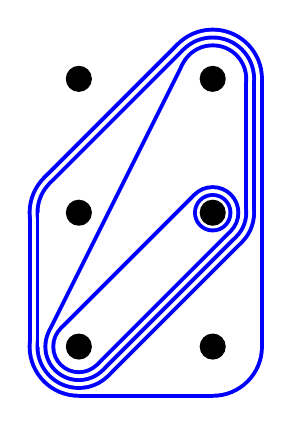
\begin{tikzpicture}
\node[fill] (1) at (0.0, 0.0) [circle] {};
\node[fill] (2) at (1.7, 0.0) [circle] {};
\node[fill] (3) at (0.0, -1.7) [circle] {};
\node[fill] (4) at (1.7, -1.7) [circle] {};
\node[fill] (5) at (0.0, -3.4) [circle] {};
\node[fill] (6) at (1.7, -3.4) [circle] {};
%23456
\begin{scope}[on background layer]
\fill[\tubecolor] (2) circle (\n + 9*\thickness);
\fill[\tubecolor] (3) circle (\n + 9*\thickness);
\fill[\tubecolor] (4) circle (\n + 9*\thickness);
\fill[\tubecolor] (5) circle (\n + 9*\thickness);
\fill[\tubecolor] (6) circle (\n + 9*\thickness);
\draw[\tubecolor] [line width = 2*(\n + 9*\thickness)] (2.center) -- (3.center);
\draw[\tubecolor] [line width = 2*(\n + 9*\thickness)] (2.center) -- (4.center);
\draw[\tubecolor] [line width = 2*(\n + 9*\thickness)] (2.center) -- (5.center);
\draw[\tubecolor] [line width = 2*(\n + 9*\thickness)] (3.center) -- (4.center);
\draw[\tubecolor] [line width = 2*(\n + 9*\thickness)] (3.center) -- (5.center);
\draw[\tubecolor] [line width = 2*(\n + 9*\thickness)] (3.center) -- (6.center);
\draw[\tubecolor] [line width = 2*(\n + 9*\thickness)] (4.center) -- (5.center);
\draw[\tubecolor] [line width = 2*(\n + 9*\thickness)] (4.center) -- (6.center);
\draw[\tubecolor] [line width = 2*(\n + 9*\thickness)] (5.center) -- (6.center);
\draw[white] [line width = 2*(\n + 8*\thickness)] (2.center) -- (3.center);
\draw[white] [line width = 2*(\n + 8*\thickness)] (2.center) -- (4.center);
\draw[white] [line width = 2*(\n + 8*\thickness)] (2.center) -- (5.center);
\draw[white] [line width = 2*(\n + 8*\thickness)] (3.center) -- (4.center);
\draw[white] [line width = 2*(\n + 8*\thickness)] (3.center) -- (5.center);
\draw[white] [line width = 2*(\n + 8*\thickness)] (3.center) -- (6.center);
\draw[white] [line width = 2*(\n + 8*\thickness)] (4.center) -- (5.center);
\draw[white] [line width = 2*(\n + 8*\thickness)] (4.center) -- (6.center);
\draw[white] [line width = 2*(\n + 8*\thickness)] (5.center) -- (6.center);
\fill[white] (2.center) -- (4.center) -- (3.center) -- (2.center);
\fill[white] (3.center) -- (5.center) -- (2.center) -- (3.center);
\fill[white] (2.center) -- (4.center) -- (5.center) -- (2.center);
\fill[white] (3.center) -- (5.center) -- (4.center) -- (3.center);
\fill[white] (4.center) -- (6.center) -- (3.center) -- (4.center);
\fill[white] (3.center) -- (5.center) -- (6.center) -- (3.center);
\fill[white] (4.center) -- (6.center) -- (5.center) -- (4.center);
\fill[white] (2) circle (\n + 8*\thickness);
\fill[white] (3) circle (\n + 8*\thickness);
\fill[white] (4) circle (\n + 8*\thickness);
\fill[white] (5) circle (\n + 8*\thickness);
\fill[white] (6) circle (\n + 8*\thickness);
\end{scope}
%2345
\begin{scope}[on background layer]
\fill[\tubecolor] (2) circle (\n + 7*\thickness);
\fill[\tubecolor] (3) circle (\n + 7*\thickness);
\fill[\tubecolor] (4) circle (\n + 7*\thickness);
\fill[\tubecolor] (5) circle (\n + 7*\thickness);
\draw[\tubecolor] [line width = 2*(\n + 7*\thickness)] (2.center) -- (3.center);
\draw[\tubecolor] [line width = 2*(\n + 7*\thickness)] (2.center) -- (4.center);
\draw[\tubecolor] [line width = 2*(\n + 7*\thickness)] (2.center) -- (5.center);
\draw[\tubecolor] [line width = 2*(\n + 7*\thickness)] (3.center) -- (4.center);
\draw[\tubecolor] [line width = 2*(\n + 7*\thickness)] (3.center) -- (5.center);
\draw[\tubecolor] [line width = 2*(\n + 7*\thickness)] (4.center) -- (5.center);
\draw[white] [line width = 2*(\n + 6*\thickness)] (2.center) -- (3.center);
\draw[white] [line width = 2*(\n + 6*\thickness)] (2.center) -- (4.center);
\draw[white] [line width = 2*(\n + 6*\thickness)] (2.center) -- (5.center);
\draw[white] [line width = 2*(\n + 6*\thickness)] (3.center) -- (4.center);
\draw[white] [line width = 2*(\n + 6*\thickness)] (3.center) -- (5.center);
\draw[white] [line width = 2*(\n + 6*\thickness)] (4.center) -- (5.center);
\fill[white] (2.center) -- (4.center) -- (3.center) -- (2.center);
\fill[white] (3.center) -- (5.center) -- (2.center) -- (3.center);
\fill[white] (2.center) -- (4.center) -- (5.center) -- (2.center);
\fill[white] (3.center) -- (5.center) -- (4.center) -- (3.center);
\fill[white] (2) circle (\n + 6*\thickness);
\fill[white] (3) circle (\n + 6*\thickness);
\fill[white] (4) circle (\n + 6*\thickness);
\fill[white] (5) circle (\n + 6*\thickness);
\end{scope}
%245
\begin{scope}[on background layer]
\fill[\tubecolor] (2) circle (\n + 5*\thickness);
\fill[\tubecolor] (4) circle (\n + 5*\thickness);
\fill[\tubecolor] (5) circle (\n + 5*\thickness);
\draw[\tubecolor] [line width = 2*(\n + 5*\thickness)] (2.center) -- (4.center);
\draw[\tubecolor] [line width = 2*(\n + 5*\thickness)] (2.center) -- (5.center);
\draw[\tubecolor] [line width = 2*(\n + 5*\thickness)] (4.center) -- (5.center);
\draw[white] [line width = 2*(\n + 4*\thickness)] (2.center) -- (4.center);
\draw[white] [line width = 2*(\n + 4*\thickness)] (2.center) -- (5.center);
\draw[white] [line width = 2*(\n + 4*\thickness)] (4.center) -- (5.center);
\fill[white] (2.center) -- (4.center) -- (5.center) -- (2.center);
\fill[white] (2) circle (\n + 4*\thickness);
\fill[white] (4) circle (\n + 4*\thickness);
\fill[white] (5) circle (\n + 4*\thickness);
\end{scope}
%45
\begin{scope}[on background layer]
\fill[\tubecolor] (4) circle (\n + 3*\thickness);
\fill[\tubecolor] (5) circle (\n + 3*\thickness);
\draw[\tubecolor] [line width = 2*(\n + 3*\thickness)] (4.center) -- (5.center);
\draw[white] [line width = 2*(\n + 2*\thickness)] (4.center) -- (5.center);
\fill[white] (4) circle (\n + 2*\thickness);
\fill[white] (5) circle (\n + 2*\thickness);
\end{scope}
%4
\begin{scope}[on background layer]
\fill[\tubecolor] (4) circle (\n + 1*\thickness);
\fill[white] (4) circle (\n + 0*\thickness);
\end{scope}
\end{tikzpicture}
%453261
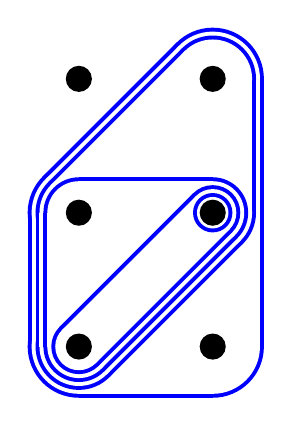
\begin{tikzpicture}
\node[fill] (1) at (0.0, 0.0) [circle] {};
\node[fill] (2) at (1.7, 0.0) [circle] {};
\node[fill] (3) at (0.0, -1.7) [circle] {};
\node[fill] (4) at (1.7, -1.7) [circle] {};
\node[fill] (5) at (0.0, -3.4) [circle] {};
\node[fill] (6) at (1.7, -3.4) [circle] {};
%23456
\begin{scope}[on background layer]
\fill[\tubecolor] (2) circle (\n + 9*\thickness);
\fill[\tubecolor] (3) circle (\n + 9*\thickness);
\fill[\tubecolor] (4) circle (\n + 9*\thickness);
\fill[\tubecolor] (5) circle (\n + 9*\thickness);
\fill[\tubecolor] (6) circle (\n + 9*\thickness);
\draw[\tubecolor] [line width = 2*(\n + 9*\thickness)] (2.center) -- (3.center);
\draw[\tubecolor] [line width = 2*(\n + 9*\thickness)] (2.center) -- (4.center);
\draw[\tubecolor] [line width = 2*(\n + 9*\thickness)] (2.center) -- (5.center);
\draw[\tubecolor] [line width = 2*(\n + 9*\thickness)] (3.center) -- (4.center);
\draw[\tubecolor] [line width = 2*(\n + 9*\thickness)] (3.center) -- (5.center);
\draw[\tubecolor] [line width = 2*(\n + 9*\thickness)] (3.center) -- (6.center);
\draw[\tubecolor] [line width = 2*(\n + 9*\thickness)] (4.center) -- (5.center);
\draw[\tubecolor] [line width = 2*(\n + 9*\thickness)] (4.center) -- (6.center);
\draw[\tubecolor] [line width = 2*(\n + 9*\thickness)] (5.center) -- (6.center);
\draw[white] [line width = 2*(\n + 8*\thickness)] (2.center) -- (3.center);
\draw[white] [line width = 2*(\n + 8*\thickness)] (2.center) -- (4.center);
\draw[white] [line width = 2*(\n + 8*\thickness)] (2.center) -- (5.center);
\draw[white] [line width = 2*(\n + 8*\thickness)] (3.center) -- (4.center);
\draw[white] [line width = 2*(\n + 8*\thickness)] (3.center) -- (5.center);
\draw[white] [line width = 2*(\n + 8*\thickness)] (3.center) -- (6.center);
\draw[white] [line width = 2*(\n + 8*\thickness)] (4.center) -- (5.center);
\draw[white] [line width = 2*(\n + 8*\thickness)] (4.center) -- (6.center);
\draw[white] [line width = 2*(\n + 8*\thickness)] (5.center) -- (6.center);
\fill[white] (2.center) -- (4.center) -- (3.center) -- (2.center);
\fill[white] (3.center) -- (5.center) -- (2.center) -- (3.center);
\fill[white] (2.center) -- (4.center) -- (5.center) -- (2.center);
\fill[white] (3.center) -- (5.center) -- (4.center) -- (3.center);
\fill[white] (4.center) -- (6.center) -- (3.center) -- (4.center);
\fill[white] (3.center) -- (5.center) -- (6.center) -- (3.center);
\fill[white] (4.center) -- (6.center) -- (5.center) -- (4.center);
\fill[white] (2) circle (\n + 8*\thickness);
\fill[white] (3) circle (\n + 8*\thickness);
\fill[white] (4) circle (\n + 8*\thickness);
\fill[white] (5) circle (\n + 8*\thickness);
\fill[white] (6) circle (\n + 8*\thickness);
\end{scope}
%2345
\begin{scope}[on background layer]
\fill[\tubecolor] (2) circle (\n + 7*\thickness);
\fill[\tubecolor] (3) circle (\n + 7*\thickness);
\fill[\tubecolor] (4) circle (\n + 7*\thickness);
\fill[\tubecolor] (5) circle (\n + 7*\thickness);
\draw[\tubecolor] [line width = 2*(\n + 7*\thickness)] (2.center) -- (3.center);
\draw[\tubecolor] [line width = 2*(\n + 7*\thickness)] (2.center) -- (4.center);
\draw[\tubecolor] [line width = 2*(\n + 7*\thickness)] (2.center) -- (5.center);
\draw[\tubecolor] [line width = 2*(\n + 7*\thickness)] (3.center) -- (4.center);
\draw[\tubecolor] [line width = 2*(\n + 7*\thickness)] (3.center) -- (5.center);
\draw[\tubecolor] [line width = 2*(\n + 7*\thickness)] (4.center) -- (5.center);
\draw[white] [line width = 2*(\n + 6*\thickness)] (2.center) -- (3.center);
\draw[white] [line width = 2*(\n + 6*\thickness)] (2.center) -- (4.center);
\draw[white] [line width = 2*(\n + 6*\thickness)] (2.center) -- (5.center);
\draw[white] [line width = 2*(\n + 6*\thickness)] (3.center) -- (4.center);
\draw[white] [line width = 2*(\n + 6*\thickness)] (3.center) -- (5.center);
\draw[white] [line width = 2*(\n + 6*\thickness)] (4.center) -- (5.center);
\fill[white] (2.center) -- (4.center) -- (3.center) -- (2.center);
\fill[white] (3.center) -- (5.center) -- (2.center) -- (3.center);
\fill[white] (2.center) -- (4.center) -- (5.center) -- (2.center);
\fill[white] (3.center) -- (5.center) -- (4.center) -- (3.center);
\fill[white] (2) circle (\n + 6*\thickness);
\fill[white] (3) circle (\n + 6*\thickness);
\fill[white] (4) circle (\n + 6*\thickness);
\fill[white] (5) circle (\n + 6*\thickness);
\end{scope}
%345
\begin{scope}[on background layer]
\fill[\tubecolor] (3) circle (\n + 5*\thickness);
\fill[\tubecolor] (4) circle (\n + 5*\thickness);
\fill[\tubecolor] (5) circle (\n + 5*\thickness);
\draw[\tubecolor] [line width = 2*(\n + 5*\thickness)] (3.center) -- (4.center);
\draw[\tubecolor] [line width = 2*(\n + 5*\thickness)] (3.center) -- (5.center);
\draw[\tubecolor] [line width = 2*(\n + 5*\thickness)] (4.center) -- (5.center);
\draw[white] [line width = 2*(\n + 4*\thickness)] (3.center) -- (4.center);
\draw[white] [line width = 2*(\n + 4*\thickness)] (3.center) -- (5.center);
\draw[white] [line width = 2*(\n + 4*\thickness)] (4.center) -- (5.center);
\fill[white] (3.center) -- (5.center) -- (4.center) -- (3.center);
\fill[white] (3) circle (\n + 4*\thickness);
\fill[white] (4) circle (\n + 4*\thickness);
\fill[white] (5) circle (\n + 4*\thickness);
\end{scope}
%45
\begin{scope}[on background layer]
\fill[\tubecolor] (4) circle (\n + 3*\thickness);
\fill[\tubecolor] (5) circle (\n + 3*\thickness);
\draw[\tubecolor] [line width = 2*(\n + 3*\thickness)] (4.center) -- (5.center);
\draw[white] [line width = 2*(\n + 2*\thickness)] (4.center) -- (5.center);
\fill[white] (4) circle (\n + 2*\thickness);
\fill[white] (5) circle (\n + 2*\thickness);
\end{scope}
%4
\begin{scope}[on background layer]
\fill[\tubecolor] (4) circle (\n + 1*\thickness);
\fill[white] (4) circle (\n + 0*\thickness);
\end{scope}
\end{tikzpicture}


%435261
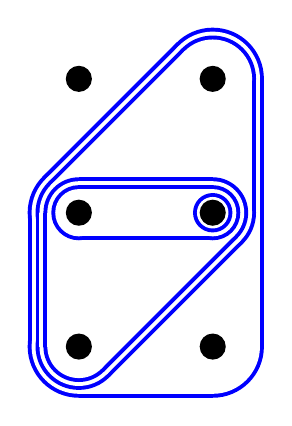
\begin{tikzpicture}
\node[fill] (1) at (0.0, 0.0) [circle] {};
\node[fill] (2) at (1.7, 0.0) [circle] {};
\node[fill] (3) at (0.0, -1.7) [circle] {};
\node[fill] (4) at (1.7, -1.7) [circle] {};
\node[fill] (5) at (0.0, -3.4) [circle] {};
\node[fill] (6) at (1.7, -3.4) [circle] {};
%23456
\begin{scope}[on background layer]
\fill[\tubecolor] (2) circle (\n + 9*\thickness);
\fill[\tubecolor] (3) circle (\n + 9*\thickness);
\fill[\tubecolor] (4) circle (\n + 9*\thickness);
\fill[\tubecolor] (5) circle (\n + 9*\thickness);
\fill[\tubecolor] (6) circle (\n + 9*\thickness);
\draw[\tubecolor] [line width = 2*(\n + 9*\thickness)] (2.center) -- (3.center);
\draw[\tubecolor] [line width = 2*(\n + 9*\thickness)] (2.center) -- (4.center);
\draw[\tubecolor] [line width = 2*(\n + 9*\thickness)] (2.center) -- (5.center);
\draw[\tubecolor] [line width = 2*(\n + 9*\thickness)] (3.center) -- (4.center);
\draw[\tubecolor] [line width = 2*(\n + 9*\thickness)] (3.center) -- (5.center);
\draw[\tubecolor] [line width = 2*(\n + 9*\thickness)] (3.center) -- (6.center);
\draw[\tubecolor] [line width = 2*(\n + 9*\thickness)] (4.center) -- (5.center);
\draw[\tubecolor] [line width = 2*(\n + 9*\thickness)] (4.center) -- (6.center);
\draw[\tubecolor] [line width = 2*(\n + 9*\thickness)] (5.center) -- (6.center);
\draw[white] [line width = 2*(\n + 8*\thickness)] (2.center) -- (3.center);
\draw[white] [line width = 2*(\n + 8*\thickness)] (2.center) -- (4.center);
\draw[white] [line width = 2*(\n + 8*\thickness)] (2.center) -- (5.center);
\draw[white] [line width = 2*(\n + 8*\thickness)] (3.center) -- (4.center);
\draw[white] [line width = 2*(\n + 8*\thickness)] (3.center) -- (5.center);
\draw[white] [line width = 2*(\n + 8*\thickness)] (3.center) -- (6.center);
\draw[white] [line width = 2*(\n + 8*\thickness)] (4.center) -- (5.center);
\draw[white] [line width = 2*(\n + 8*\thickness)] (4.center) -- (6.center);
\draw[white] [line width = 2*(\n + 8*\thickness)] (5.center) -- (6.center);
\fill[white] (2.center) -- (4.center) -- (3.center) -- (2.center);
\fill[white] (3.center) -- (5.center) -- (2.center) -- (3.center);
\fill[white] (2.center) -- (4.center) -- (5.center) -- (2.center);
\fill[white] (3.center) -- (5.center) -- (4.center) -- (3.center);
\fill[white] (4.center) -- (6.center) -- (3.center) -- (4.center);
\fill[white] (3.center) -- (5.center) -- (6.center) -- (3.center);
\fill[white] (4.center) -- (6.center) -- (5.center) -- (4.center);
\fill[white] (2) circle (\n + 8*\thickness);
\fill[white] (3) circle (\n + 8*\thickness);
\fill[white] (4) circle (\n + 8*\thickness);
\fill[white] (5) circle (\n + 8*\thickness);
\fill[white] (6) circle (\n + 8*\thickness);
\end{scope}
%2345
\begin{scope}[on background layer]
\fill[\tubecolor] (2) circle (\n + 7*\thickness);
\fill[\tubecolor] (3) circle (\n + 7*\thickness);
\fill[\tubecolor] (4) circle (\n + 7*\thickness);
\fill[\tubecolor] (5) circle (\n + 7*\thickness);
\draw[\tubecolor] [line width = 2*(\n + 7*\thickness)] (2.center) -- (3.center);
\draw[\tubecolor] [line width = 2*(\n + 7*\thickness)] (2.center) -- (4.center);
\draw[\tubecolor] [line width = 2*(\n + 7*\thickness)] (2.center) -- (5.center);
\draw[\tubecolor] [line width = 2*(\n + 7*\thickness)] (3.center) -- (4.center);
\draw[\tubecolor] [line width = 2*(\n + 7*\thickness)] (3.center) -- (5.center);
\draw[\tubecolor] [line width = 2*(\n + 7*\thickness)] (4.center) -- (5.center);
\draw[white] [line width = 2*(\n + 6*\thickness)] (2.center) -- (3.center);
\draw[white] [line width = 2*(\n + 6*\thickness)] (2.center) -- (4.center);
\draw[white] [line width = 2*(\n + 6*\thickness)] (2.center) -- (5.center);
\draw[white] [line width = 2*(\n + 6*\thickness)] (3.center) -- (4.center);
\draw[white] [line width = 2*(\n + 6*\thickness)] (3.center) -- (5.center);
\draw[white] [line width = 2*(\n + 6*\thickness)] (4.center) -- (5.center);
\fill[white] (2.center) -- (4.center) -- (3.center) -- (2.center);
\fill[white] (3.center) -- (5.center) -- (2.center) -- (3.center);
\fill[white] (2.center) -- (4.center) -- (5.center) -- (2.center);
\fill[white] (3.center) -- (5.center) -- (4.center) -- (3.center);
\fill[white] (2) circle (\n + 6*\thickness);
\fill[white] (3) circle (\n + 6*\thickness);
\fill[white] (4) circle (\n + 6*\thickness);
\fill[white] (5) circle (\n + 6*\thickness);
\end{scope}
%345
\begin{scope}[on background layer]
\fill[\tubecolor] (3) circle (\n + 5*\thickness);
\fill[\tubecolor] (4) circle (\n + 5*\thickness);
\fill[\tubecolor] (5) circle (\n + 5*\thickness);
\draw[\tubecolor] [line width = 2*(\n + 5*\thickness)] (3.center) -- (4.center);
\draw[\tubecolor] [line width = 2*(\n + 5*\thickness)] (3.center) -- (5.center);
\draw[\tubecolor] [line width = 2*(\n + 5*\thickness)] (4.center) -- (5.center);
\draw[white] [line width = 2*(\n + 4*\thickness)] (3.center) -- (4.center);
\draw[white] [line width = 2*(\n + 4*\thickness)] (3.center) -- (5.center);
\draw[white] [line width = 2*(\n + 4*\thickness)] (4.center) -- (5.center);
\fill[white] (3.center) -- (5.center) -- (4.center) -- (3.center);
\fill[white] (3) circle (\n + 4*\thickness);
\fill[white] (4) circle (\n + 4*\thickness);
\fill[white] (5) circle (\n + 4*\thickness);
\end{scope}
%34
\begin{scope}[on background layer]
\fill[\tubecolor] (3) circle (\n + 3*\thickness);
\fill[\tubecolor] (4) circle (\n + 3*\thickness);
\draw[\tubecolor] [line width = 2*(\n + 3*\thickness)] (3.center) -- (4.center);
\draw[white] [line width = 2*(\n + 2*\thickness)] (3.center) -- (4.center);
\fill[white] (3) circle (\n + 2*\thickness);
\fill[white] (4) circle (\n + 2*\thickness);
\end{scope}
%4
\begin{scope}[on background layer]
\fill[\tubecolor] (4) circle (\n + 1*\thickness);
\fill[white] (4) circle (\n + 0*\thickness);
\end{scope}
\end{tikzpicture}
%345261
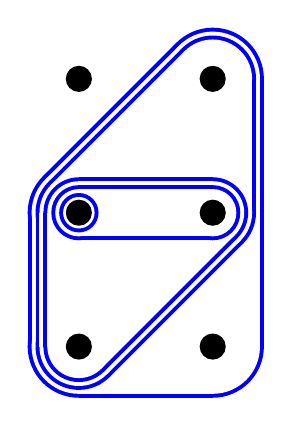
\begin{tikzpicture}
\node[fill] (1) at (0.0, 0.0) [circle] {};
\node[fill] (2) at (1.7, 0.0) [circle] {};
\node[fill] (3) at (0.0, -1.7) [circle] {};
\node[fill] (4) at (1.7, -1.7) [circle] {};
\node[fill] (5) at (0.0, -3.4) [circle] {};
\node[fill] (6) at (1.7, -3.4) [circle] {};
%23456
\begin{scope}[on background layer]
\fill[\tubecolor] (2) circle (\n + 9*\thickness);
\fill[\tubecolor] (3) circle (\n + 9*\thickness);
\fill[\tubecolor] (4) circle (\n + 9*\thickness);
\fill[\tubecolor] (5) circle (\n + 9*\thickness);
\fill[\tubecolor] (6) circle (\n + 9*\thickness);
\draw[\tubecolor] [line width = 2*(\n + 9*\thickness)] (2.center) -- (3.center);
\draw[\tubecolor] [line width = 2*(\n + 9*\thickness)] (2.center) -- (4.center);
\draw[\tubecolor] [line width = 2*(\n + 9*\thickness)] (2.center) -- (5.center);
\draw[\tubecolor] [line width = 2*(\n + 9*\thickness)] (3.center) -- (4.center);
\draw[\tubecolor] [line width = 2*(\n + 9*\thickness)] (3.center) -- (5.center);
\draw[\tubecolor] [line width = 2*(\n + 9*\thickness)] (3.center) -- (6.center);
\draw[\tubecolor] [line width = 2*(\n + 9*\thickness)] (4.center) -- (5.center);
\draw[\tubecolor] [line width = 2*(\n + 9*\thickness)] (4.center) -- (6.center);
\draw[\tubecolor] [line width = 2*(\n + 9*\thickness)] (5.center) -- (6.center);
\draw[white] [line width = 2*(\n + 8*\thickness)] (2.center) -- (3.center);
\draw[white] [line width = 2*(\n + 8*\thickness)] (2.center) -- (4.center);
\draw[white] [line width = 2*(\n + 8*\thickness)] (2.center) -- (5.center);
\draw[white] [line width = 2*(\n + 8*\thickness)] (3.center) -- (4.center);
\draw[white] [line width = 2*(\n + 8*\thickness)] (3.center) -- (5.center);
\draw[white] [line width = 2*(\n + 8*\thickness)] (3.center) -- (6.center);
\draw[white] [line width = 2*(\n + 8*\thickness)] (4.center) -- (5.center);
\draw[white] [line width = 2*(\n + 8*\thickness)] (4.center) -- (6.center);
\draw[white] [line width = 2*(\n + 8*\thickness)] (5.center) -- (6.center);
\fill[white] (2.center) -- (4.center) -- (3.center) -- (2.center);
\fill[white] (3.center) -- (5.center) -- (2.center) -- (3.center);
\fill[white] (2.center) -- (4.center) -- (5.center) -- (2.center);
\fill[white] (3.center) -- (5.center) -- (4.center) -- (3.center);
\fill[white] (4.center) -- (6.center) -- (3.center) -- (4.center);
\fill[white] (3.center) -- (5.center) -- (6.center) -- (3.center);
\fill[white] (4.center) -- (6.center) -- (5.center) -- (4.center);
\fill[white] (2) circle (\n + 8*\thickness);
\fill[white] (3) circle (\n + 8*\thickness);
\fill[white] (4) circle (\n + 8*\thickness);
\fill[white] (5) circle (\n + 8*\thickness);
\fill[white] (6) circle (\n + 8*\thickness);
\end{scope}
%2345
\begin{scope}[on background layer]
\fill[\tubecolor] (2) circle (\n + 7*\thickness);
\fill[\tubecolor] (3) circle (\n + 7*\thickness);
\fill[\tubecolor] (4) circle (\n + 7*\thickness);
\fill[\tubecolor] (5) circle (\n + 7*\thickness);
\draw[\tubecolor] [line width = 2*(\n + 7*\thickness)] (2.center) -- (3.center);
\draw[\tubecolor] [line width = 2*(\n + 7*\thickness)] (2.center) -- (4.center);
\draw[\tubecolor] [line width = 2*(\n + 7*\thickness)] (2.center) -- (5.center);
\draw[\tubecolor] [line width = 2*(\n + 7*\thickness)] (3.center) -- (4.center);
\draw[\tubecolor] [line width = 2*(\n + 7*\thickness)] (3.center) -- (5.center);
\draw[\tubecolor] [line width = 2*(\n + 7*\thickness)] (4.center) -- (5.center);
\draw[white] [line width = 2*(\n + 6*\thickness)] (2.center) -- (3.center);
\draw[white] [line width = 2*(\n + 6*\thickness)] (2.center) -- (4.center);
\draw[white] [line width = 2*(\n + 6*\thickness)] (2.center) -- (5.center);
\draw[white] [line width = 2*(\n + 6*\thickness)] (3.center) -- (4.center);
\draw[white] [line width = 2*(\n + 6*\thickness)] (3.center) -- (5.center);
\draw[white] [line width = 2*(\n + 6*\thickness)] (4.center) -- (5.center);
\fill[white] (2.center) -- (4.center) -- (3.center) -- (2.center);
\fill[white] (3.center) -- (5.center) -- (2.center) -- (3.center);
\fill[white] (2.center) -- (4.center) -- (5.center) -- (2.center);
\fill[white] (3.center) -- (5.center) -- (4.center) -- (3.center);
\fill[white] (2) circle (\n + 6*\thickness);
\fill[white] (3) circle (\n + 6*\thickness);
\fill[white] (4) circle (\n + 6*\thickness);
\fill[white] (5) circle (\n + 6*\thickness);
\end{scope}
%345
\begin{scope}[on background layer]
\fill[\tubecolor] (3) circle (\n + 5*\thickness);
\fill[\tubecolor] (4) circle (\n + 5*\thickness);
\fill[\tubecolor] (5) circle (\n + 5*\thickness);
\draw[\tubecolor] [line width = 2*(\n + 5*\thickness)] (3.center) -- (4.center);
\draw[\tubecolor] [line width = 2*(\n + 5*\thickness)] (3.center) -- (5.center);
\draw[\tubecolor] [line width = 2*(\n + 5*\thickness)] (4.center) -- (5.center);
\draw[white] [line width = 2*(\n + 4*\thickness)] (3.center) -- (4.center);
\draw[white] [line width = 2*(\n + 4*\thickness)] (3.center) -- (5.center);
\draw[white] [line width = 2*(\n + 4*\thickness)] (4.center) -- (5.center);
\fill[white] (3.center) -- (5.center) -- (4.center) -- (3.center);
\fill[white] (3) circle (\n + 4*\thickness);
\fill[white] (4) circle (\n + 4*\thickness);
\fill[white] (5) circle (\n + 4*\thickness);
\end{scope}
%34
\begin{scope}[on background layer]
\fill[\tubecolor] (3) circle (\n + 3*\thickness);
\fill[\tubecolor] (4) circle (\n + 3*\thickness);
\draw[\tubecolor] [line width = 2*(\n + 3*\thickness)] (3.center) -- (4.center);
\draw[white] [line width = 2*(\n + 2*\thickness)] (3.center) -- (4.center);
\fill[white] (3) circle (\n + 2*\thickness);
\fill[white] (4) circle (\n + 2*\thickness);
\end{scope}
%3
\begin{scope}[on background layer]
\fill[\tubecolor] (3) circle (\n + 1*\thickness);
\fill[white] (3) circle (\n + 0*\thickness);
\end{scope}
\end{tikzpicture}
%342561
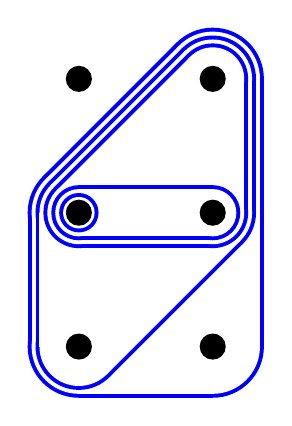
\begin{tikzpicture}
\node[fill] (1) at (0.0, 0.0) [circle] {};
\node[fill] (2) at (1.7, 0.0) [circle] {};
\node[fill] (3) at (0.0, -1.7) [circle] {};
\node[fill] (4) at (1.7, -1.7) [circle] {};
\node[fill] (5) at (0.0, -3.4) [circle] {};
\node[fill] (6) at (1.7, -3.4) [circle] {};
%23456
\begin{scope}[on background layer]
\fill[\tubecolor] (2) circle (\n + 9*\thickness);
\fill[\tubecolor] (3) circle (\n + 9*\thickness);
\fill[\tubecolor] (4) circle (\n + 9*\thickness);
\fill[\tubecolor] (5) circle (\n + 9*\thickness);
\fill[\tubecolor] (6) circle (\n + 9*\thickness);
\draw[\tubecolor] [line width = 2*(\n + 9*\thickness)] (2.center) -- (3.center);
\draw[\tubecolor] [line width = 2*(\n + 9*\thickness)] (2.center) -- (4.center);
\draw[\tubecolor] [line width = 2*(\n + 9*\thickness)] (2.center) -- (5.center);
\draw[\tubecolor] [line width = 2*(\n + 9*\thickness)] (3.center) -- (4.center);
\draw[\tubecolor] [line width = 2*(\n + 9*\thickness)] (3.center) -- (5.center);
\draw[\tubecolor] [line width = 2*(\n + 9*\thickness)] (3.center) -- (6.center);
\draw[\tubecolor] [line width = 2*(\n + 9*\thickness)] (4.center) -- (5.center);
\draw[\tubecolor] [line width = 2*(\n + 9*\thickness)] (4.center) -- (6.center);
\draw[\tubecolor] [line width = 2*(\n + 9*\thickness)] (5.center) -- (6.center);
\draw[white] [line width = 2*(\n + 8*\thickness)] (2.center) -- (3.center);
\draw[white] [line width = 2*(\n + 8*\thickness)] (2.center) -- (4.center);
\draw[white] [line width = 2*(\n + 8*\thickness)] (2.center) -- (5.center);
\draw[white] [line width = 2*(\n + 8*\thickness)] (3.center) -- (4.center);
\draw[white] [line width = 2*(\n + 8*\thickness)] (3.center) -- (5.center);
\draw[white] [line width = 2*(\n + 8*\thickness)] (3.center) -- (6.center);
\draw[white] [line width = 2*(\n + 8*\thickness)] (4.center) -- (5.center);
\draw[white] [line width = 2*(\n + 8*\thickness)] (4.center) -- (6.center);
\draw[white] [line width = 2*(\n + 8*\thickness)] (5.center) -- (6.center);
\fill[white] (2.center) -- (4.center) -- (3.center) -- (2.center);
\fill[white] (3.center) -- (5.center) -- (2.center) -- (3.center);
\fill[white] (2.center) -- (4.center) -- (5.center) -- (2.center);
\fill[white] (3.center) -- (5.center) -- (4.center) -- (3.center);
\fill[white] (4.center) -- (6.center) -- (3.center) -- (4.center);
\fill[white] (3.center) -- (5.center) -- (6.center) -- (3.center);
\fill[white] (4.center) -- (6.center) -- (5.center) -- (4.center);
\fill[white] (2) circle (\n + 8*\thickness);
\fill[white] (3) circle (\n + 8*\thickness);
\fill[white] (4) circle (\n + 8*\thickness);
\fill[white] (5) circle (\n + 8*\thickness);
\fill[white] (6) circle (\n + 8*\thickness);
\end{scope}
%2345
\begin{scope}[on background layer]
\fill[\tubecolor] (2) circle (\n + 7*\thickness);
\fill[\tubecolor] (3) circle (\n + 7*\thickness);
\fill[\tubecolor] (4) circle (\n + 7*\thickness);
\fill[\tubecolor] (5) circle (\n + 7*\thickness);
\draw[\tubecolor] [line width = 2*(\n + 7*\thickness)] (2.center) -- (3.center);
\draw[\tubecolor] [line width = 2*(\n + 7*\thickness)] (2.center) -- (4.center);
\draw[\tubecolor] [line width = 2*(\n + 7*\thickness)] (2.center) -- (5.center);
\draw[\tubecolor] [line width = 2*(\n + 7*\thickness)] (3.center) -- (4.center);
\draw[\tubecolor] [line width = 2*(\n + 7*\thickness)] (3.center) -- (5.center);
\draw[\tubecolor] [line width = 2*(\n + 7*\thickness)] (4.center) -- (5.center);
\draw[white] [line width = 2*(\n + 6*\thickness)] (2.center) -- (3.center);
\draw[white] [line width = 2*(\n + 6*\thickness)] (2.center) -- (4.center);
\draw[white] [line width = 2*(\n + 6*\thickness)] (2.center) -- (5.center);
\draw[white] [line width = 2*(\n + 6*\thickness)] (3.center) -- (4.center);
\draw[white] [line width = 2*(\n + 6*\thickness)] (3.center) -- (5.center);
\draw[white] [line width = 2*(\n + 6*\thickness)] (4.center) -- (5.center);
\fill[white] (2.center) -- (4.center) -- (3.center) -- (2.center);
\fill[white] (3.center) -- (5.center) -- (2.center) -- (3.center);
\fill[white] (2.center) -- (4.center) -- (5.center) -- (2.center);
\fill[white] (3.center) -- (5.center) -- (4.center) -- (3.center);
\fill[white] (2) circle (\n + 6*\thickness);
\fill[white] (3) circle (\n + 6*\thickness);
\fill[white] (4) circle (\n + 6*\thickness);
\fill[white] (5) circle (\n + 6*\thickness);
\end{scope}
%234
\begin{scope}[on background layer]
\fill[\tubecolor] (2) circle (\n + 5*\thickness);
\fill[\tubecolor] (3) circle (\n + 5*\thickness);
\fill[\tubecolor] (4) circle (\n + 5*\thickness);
\draw[\tubecolor] [line width = 2*(\n + 5*\thickness)] (2.center) -- (3.center);
\draw[\tubecolor] [line width = 2*(\n + 5*\thickness)] (2.center) -- (4.center);
\draw[\tubecolor] [line width = 2*(\n + 5*\thickness)] (3.center) -- (4.center);
\draw[white] [line width = 2*(\n + 4*\thickness)] (2.center) -- (3.center);
\draw[white] [line width = 2*(\n + 4*\thickness)] (2.center) -- (4.center);
\draw[white] [line width = 2*(\n + 4*\thickness)] (3.center) -- (4.center);
\fill[white] (2.center) -- (4.center) -- (3.center) -- (2.center);
\fill[white] (2) circle (\n + 4*\thickness);
\fill[white] (3) circle (\n + 4*\thickness);
\fill[white] (4) circle (\n + 4*\thickness);
\end{scope}
%34
\begin{scope}[on background layer]
\fill[\tubecolor] (3) circle (\n + 3*\thickness);
\fill[\tubecolor] (4) circle (\n + 3*\thickness);
\draw[\tubecolor] [line width = 2*(\n + 3*\thickness)] (3.center) -- (4.center);
\draw[white] [line width = 2*(\n + 2*\thickness)] (3.center) -- (4.center);
\fill[white] (3) circle (\n + 2*\thickness);
\fill[white] (4) circle (\n + 2*\thickness);
\end{scope}
%3
\begin{scope}[on background layer]
\fill[\tubecolor] (3) circle (\n + 1*\thickness);
\fill[white] (3) circle (\n + 0*\thickness);
\end{scope}
\end{tikzpicture}
%324561
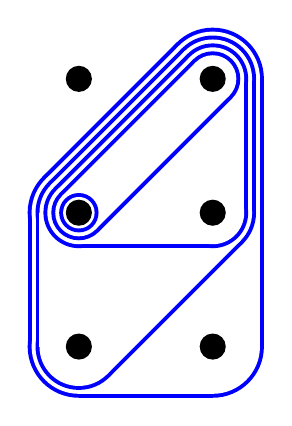
\begin{tikzpicture}
\node[fill] (1) at (0.0, 0.0) [circle] {};
\node[fill] (2) at (1.7, 0.0) [circle] {};
\node[fill] (3) at (0.0, -1.7) [circle] {};
\node[fill] (4) at (1.7, -1.7) [circle] {};
\node[fill] (5) at (0.0, -3.4) [circle] {};
\node[fill] (6) at (1.7, -3.4) [circle] {};
%23456
\begin{scope}[on background layer]
\fill[\tubecolor] (2) circle (\n + 9*\thickness);
\fill[\tubecolor] (3) circle (\n + 9*\thickness);
\fill[\tubecolor] (4) circle (\n + 9*\thickness);
\fill[\tubecolor] (5) circle (\n + 9*\thickness);
\fill[\tubecolor] (6) circle (\n + 9*\thickness);
\draw[\tubecolor] [line width = 2*(\n + 9*\thickness)] (2.center) -- (3.center);
\draw[\tubecolor] [line width = 2*(\n + 9*\thickness)] (2.center) -- (4.center);
\draw[\tubecolor] [line width = 2*(\n + 9*\thickness)] (2.center) -- (5.center);
\draw[\tubecolor] [line width = 2*(\n + 9*\thickness)] (3.center) -- (4.center);
\draw[\tubecolor] [line width = 2*(\n + 9*\thickness)] (3.center) -- (5.center);
\draw[\tubecolor] [line width = 2*(\n + 9*\thickness)] (3.center) -- (6.center);
\draw[\tubecolor] [line width = 2*(\n + 9*\thickness)] (4.center) -- (5.center);
\draw[\tubecolor] [line width = 2*(\n + 9*\thickness)] (4.center) -- (6.center);
\draw[\tubecolor] [line width = 2*(\n + 9*\thickness)] (5.center) -- (6.center);
\draw[white] [line width = 2*(\n + 8*\thickness)] (2.center) -- (3.center);
\draw[white] [line width = 2*(\n + 8*\thickness)] (2.center) -- (4.center);
\draw[white] [line width = 2*(\n + 8*\thickness)] (2.center) -- (5.center);
\draw[white] [line width = 2*(\n + 8*\thickness)] (3.center) -- (4.center);
\draw[white] [line width = 2*(\n + 8*\thickness)] (3.center) -- (5.center);
\draw[white] [line width = 2*(\n + 8*\thickness)] (3.center) -- (6.center);
\draw[white] [line width = 2*(\n + 8*\thickness)] (4.center) -- (5.center);
\draw[white] [line width = 2*(\n + 8*\thickness)] (4.center) -- (6.center);
\draw[white] [line width = 2*(\n + 8*\thickness)] (5.center) -- (6.center);
\fill[white] (2.center) -- (4.center) -- (3.center) -- (2.center);
\fill[white] (3.center) -- (5.center) -- (2.center) -- (3.center);
\fill[white] (2.center) -- (4.center) -- (5.center) -- (2.center);
\fill[white] (3.center) -- (5.center) -- (4.center) -- (3.center);
\fill[white] (4.center) -- (6.center) -- (3.center) -- (4.center);
\fill[white] (3.center) -- (5.center) -- (6.center) -- (3.center);
\fill[white] (4.center) -- (6.center) -- (5.center) -- (4.center);
\fill[white] (2) circle (\n + 8*\thickness);
\fill[white] (3) circle (\n + 8*\thickness);
\fill[white] (4) circle (\n + 8*\thickness);
\fill[white] (5) circle (\n + 8*\thickness);
\fill[white] (6) circle (\n + 8*\thickness);
\end{scope}
%2345
\begin{scope}[on background layer]
\fill[\tubecolor] (2) circle (\n + 7*\thickness);
\fill[\tubecolor] (3) circle (\n + 7*\thickness);
\fill[\tubecolor] (4) circle (\n + 7*\thickness);
\fill[\tubecolor] (5) circle (\n + 7*\thickness);
\draw[\tubecolor] [line width = 2*(\n + 7*\thickness)] (2.center) -- (3.center);
\draw[\tubecolor] [line width = 2*(\n + 7*\thickness)] (2.center) -- (4.center);
\draw[\tubecolor] [line width = 2*(\n + 7*\thickness)] (2.center) -- (5.center);
\draw[\tubecolor] [line width = 2*(\n + 7*\thickness)] (3.center) -- (4.center);
\draw[\tubecolor] [line width = 2*(\n + 7*\thickness)] (3.center) -- (5.center);
\draw[\tubecolor] [line width = 2*(\n + 7*\thickness)] (4.center) -- (5.center);
\draw[white] [line width = 2*(\n + 6*\thickness)] (2.center) -- (3.center);
\draw[white] [line width = 2*(\n + 6*\thickness)] (2.center) -- (4.center);
\draw[white] [line width = 2*(\n + 6*\thickness)] (2.center) -- (5.center);
\draw[white] [line width = 2*(\n + 6*\thickness)] (3.center) -- (4.center);
\draw[white] [line width = 2*(\n + 6*\thickness)] (3.center) -- (5.center);
\draw[white] [line width = 2*(\n + 6*\thickness)] (4.center) -- (5.center);
\fill[white] (2.center) -- (4.center) -- (3.center) -- (2.center);
\fill[white] (3.center) -- (5.center) -- (2.center) -- (3.center);
\fill[white] (2.center) -- (4.center) -- (5.center) -- (2.center);
\fill[white] (3.center) -- (5.center) -- (4.center) -- (3.center);
\fill[white] (2) circle (\n + 6*\thickness);
\fill[white] (3) circle (\n + 6*\thickness);
\fill[white] (4) circle (\n + 6*\thickness);
\fill[white] (5) circle (\n + 6*\thickness);
\end{scope}
%234
\begin{scope}[on background layer]
\fill[\tubecolor] (2) circle (\n + 5*\thickness);
\fill[\tubecolor] (3) circle (\n + 5*\thickness);
\fill[\tubecolor] (4) circle (\n + 5*\thickness);
\draw[\tubecolor] [line width = 2*(\n + 5*\thickness)] (2.center) -- (3.center);
\draw[\tubecolor] [line width = 2*(\n + 5*\thickness)] (2.center) -- (4.center);
\draw[\tubecolor] [line width = 2*(\n + 5*\thickness)] (3.center) -- (4.center);
\draw[white] [line width = 2*(\n + 4*\thickness)] (2.center) -- (3.center);
\draw[white] [line width = 2*(\n + 4*\thickness)] (2.center) -- (4.center);
\draw[white] [line width = 2*(\n + 4*\thickness)] (3.center) -- (4.center);
\fill[white] (2.center) -- (4.center) -- (3.center) -- (2.center);
\fill[white] (2) circle (\n + 4*\thickness);
\fill[white] (3) circle (\n + 4*\thickness);
\fill[white] (4) circle (\n + 4*\thickness);
\end{scope}
%23
\begin{scope}[on background layer]
\fill[\tubecolor] (2) circle (\n + 3*\thickness);
\fill[\tubecolor] (3) circle (\n + 3*\thickness);
\draw[\tubecolor] [line width = 2*(\n + 3*\thickness)] (2.center) -- (3.center);
\draw[white] [line width = 2*(\n + 2*\thickness)] (2.center) -- (3.center);
\fill[white] (2) circle (\n + 2*\thickness);
\fill[white] (3) circle (\n + 2*\thickness);
\end{scope}
%3
\begin{scope}[on background layer]
\fill[\tubecolor] (3) circle (\n + 1*\thickness);
\fill[white] (3) circle (\n + 0*\thickness);
\end{scope}
\end{tikzpicture}
%234561
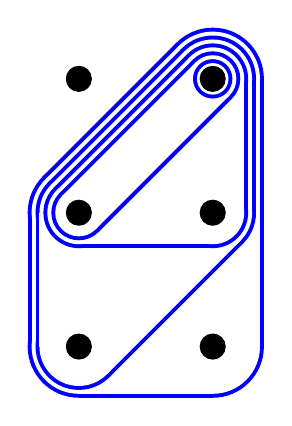
\begin{tikzpicture}
\node[fill] (1) at (0.0, 0.0) [circle] {};
\node[fill] (2) at (1.7, 0.0) [circle] {};
\node[fill] (3) at (0.0, -1.7) [circle] {};
\node[fill] (4) at (1.7, -1.7) [circle] {};
\node[fill] (5) at (0.0, -3.4) [circle] {};
\node[fill] (6) at (1.7, -3.4) [circle] {};
%23456
\begin{scope}[on background layer]
\fill[\tubecolor] (2) circle (\n + 9*\thickness);
\fill[\tubecolor] (3) circle (\n + 9*\thickness);
\fill[\tubecolor] (4) circle (\n + 9*\thickness);
\fill[\tubecolor] (5) circle (\n + 9*\thickness);
\fill[\tubecolor] (6) circle (\n + 9*\thickness);
\draw[\tubecolor] [line width = 2*(\n + 9*\thickness)] (2.center) -- (3.center);
\draw[\tubecolor] [line width = 2*(\n + 9*\thickness)] (2.center) -- (4.center);
\draw[\tubecolor] [line width = 2*(\n + 9*\thickness)] (2.center) -- (5.center);
\draw[\tubecolor] [line width = 2*(\n + 9*\thickness)] (3.center) -- (4.center);
\draw[\tubecolor] [line width = 2*(\n + 9*\thickness)] (3.center) -- (5.center);
\draw[\tubecolor] [line width = 2*(\n + 9*\thickness)] (3.center) -- (6.center);
\draw[\tubecolor] [line width = 2*(\n + 9*\thickness)] (4.center) -- (5.center);
\draw[\tubecolor] [line width = 2*(\n + 9*\thickness)] (4.center) -- (6.center);
\draw[\tubecolor] [line width = 2*(\n + 9*\thickness)] (5.center) -- (6.center);
\draw[white] [line width = 2*(\n + 8*\thickness)] (2.center) -- (3.center);
\draw[white] [line width = 2*(\n + 8*\thickness)] (2.center) -- (4.center);
\draw[white] [line width = 2*(\n + 8*\thickness)] (2.center) -- (5.center);
\draw[white] [line width = 2*(\n + 8*\thickness)] (3.center) -- (4.center);
\draw[white] [line width = 2*(\n + 8*\thickness)] (3.center) -- (5.center);
\draw[white] [line width = 2*(\n + 8*\thickness)] (3.center) -- (6.center);
\draw[white] [line width = 2*(\n + 8*\thickness)] (4.center) -- (5.center);
\draw[white] [line width = 2*(\n + 8*\thickness)] (4.center) -- (6.center);
\draw[white] [line width = 2*(\n + 8*\thickness)] (5.center) -- (6.center);
\fill[white] (2.center) -- (4.center) -- (3.center) -- (2.center);
\fill[white] (3.center) -- (5.center) -- (2.center) -- (3.center);
\fill[white] (2.center) -- (4.center) -- (5.center) -- (2.center);
\fill[white] (3.center) -- (5.center) -- (4.center) -- (3.center);
\fill[white] (4.center) -- (6.center) -- (3.center) -- (4.center);
\fill[white] (3.center) -- (5.center) -- (6.center) -- (3.center);
\fill[white] (4.center) -- (6.center) -- (5.center) -- (4.center);
\fill[white] (2) circle (\n + 8*\thickness);
\fill[white] (3) circle (\n + 8*\thickness);
\fill[white] (4) circle (\n + 8*\thickness);
\fill[white] (5) circle (\n + 8*\thickness);
\fill[white] (6) circle (\n + 8*\thickness);
\end{scope}
%2345
\begin{scope}[on background layer]
\fill[\tubecolor] (2) circle (\n + 7*\thickness);
\fill[\tubecolor] (3) circle (\n + 7*\thickness);
\fill[\tubecolor] (4) circle (\n + 7*\thickness);
\fill[\tubecolor] (5) circle (\n + 7*\thickness);
\draw[\tubecolor] [line width = 2*(\n + 7*\thickness)] (2.center) -- (3.center);
\draw[\tubecolor] [line width = 2*(\n + 7*\thickness)] (2.center) -- (4.center);
\draw[\tubecolor] [line width = 2*(\n + 7*\thickness)] (2.center) -- (5.center);
\draw[\tubecolor] [line width = 2*(\n + 7*\thickness)] (3.center) -- (4.center);
\draw[\tubecolor] [line width = 2*(\n + 7*\thickness)] (3.center) -- (5.center);
\draw[\tubecolor] [line width = 2*(\n + 7*\thickness)] (4.center) -- (5.center);
\draw[white] [line width = 2*(\n + 6*\thickness)] (2.center) -- (3.center);
\draw[white] [line width = 2*(\n + 6*\thickness)] (2.center) -- (4.center);
\draw[white] [line width = 2*(\n + 6*\thickness)] (2.center) -- (5.center);
\draw[white] [line width = 2*(\n + 6*\thickness)] (3.center) -- (4.center);
\draw[white] [line width = 2*(\n + 6*\thickness)] (3.center) -- (5.center);
\draw[white] [line width = 2*(\n + 6*\thickness)] (4.center) -- (5.center);
\fill[white] (2.center) -- (4.center) -- (3.center) -- (2.center);
\fill[white] (3.center) -- (5.center) -- (2.center) -- (3.center);
\fill[white] (2.center) -- (4.center) -- (5.center) -- (2.center);
\fill[white] (3.center) -- (5.center) -- (4.center) -- (3.center);
\fill[white] (2) circle (\n + 6*\thickness);
\fill[white] (3) circle (\n + 6*\thickness);
\fill[white] (4) circle (\n + 6*\thickness);
\fill[white] (5) circle (\n + 6*\thickness);
\end{scope}
%234
\begin{scope}[on background layer]
\fill[\tubecolor] (2) circle (\n + 5*\thickness);
\fill[\tubecolor] (3) circle (\n + 5*\thickness);
\fill[\tubecolor] (4) circle (\n + 5*\thickness);
\draw[\tubecolor] [line width = 2*(\n + 5*\thickness)] (2.center) -- (3.center);
\draw[\tubecolor] [line width = 2*(\n + 5*\thickness)] (2.center) -- (4.center);
\draw[\tubecolor] [line width = 2*(\n + 5*\thickness)] (3.center) -- (4.center);
\draw[white] [line width = 2*(\n + 4*\thickness)] (2.center) -- (3.center);
\draw[white] [line width = 2*(\n + 4*\thickness)] (2.center) -- (4.center);
\draw[white] [line width = 2*(\n + 4*\thickness)] (3.center) -- (4.center);
\fill[white] (2.center) -- (4.center) -- (3.center) -- (2.center);
\fill[white] (2) circle (\n + 4*\thickness);
\fill[white] (3) circle (\n + 4*\thickness);
\fill[white] (4) circle (\n + 4*\thickness);
\end{scope}
%23
\begin{scope}[on background layer]
\fill[\tubecolor] (2) circle (\n + 3*\thickness);
\fill[\tubecolor] (3) circle (\n + 3*\thickness);
\draw[\tubecolor] [line width = 2*(\n + 3*\thickness)] (2.center) -- (3.center);
\draw[white] [line width = 2*(\n + 2*\thickness)] (2.center) -- (3.center);
\fill[white] (2) circle (\n + 2*\thickness);
\fill[white] (3) circle (\n + 2*\thickness);
\end{scope}
%2
\begin{scope}[on background layer]
\fill[\tubecolor] (2) circle (\n + 1*\thickness);
\fill[white] (2) circle (\n + 0*\thickness);
\end{scope}
\end{tikzpicture}
%234516
\begin{tikzpicture}
\node[fill] (1) at (0.0, 0.0) [circle] {};
\node[fill] (2) at (1.7, 0.0) [circle] {};
\node[fill] (3) at (0.0, -1.7) [circle] {};
\node[fill] (4) at (1.7, -1.7) [circle] {};
\node[fill] (5) at (0.0, -3.4) [circle] {};
\node[fill] (6) at (1.7, -3.4) [circle] {};
%12345
\begin{scope}[on background layer]
\fill[\tubecolor] (1) circle (\n + 9*\thickness);
\fill[\tubecolor] (2) circle (\n + 9*\thickness);
\fill[\tubecolor] (3) circle (\n + 9*\thickness);
\fill[\tubecolor] (4) circle (\n + 9*\thickness);
\fill[\tubecolor] (5) circle (\n + 9*\thickness);
\draw[\tubecolor] [line width = 2*(\n + 9*\thickness)] (1.center) -- (2.center);
\draw[\tubecolor] [line width = 2*(\n + 9*\thickness)] (1.center) -- (3.center);
\draw[\tubecolor] [line width = 2*(\n + 9*\thickness)] (1.center) -- (4.center);
\draw[\tubecolor] [line width = 2*(\n + 9*\thickness)] (2.center) -- (3.center);
\draw[\tubecolor] [line width = 2*(\n + 9*\thickness)] (2.center) -- (4.center);
\draw[\tubecolor] [line width = 2*(\n + 9*\thickness)] (2.center) -- (5.center);
\draw[\tubecolor] [line width = 2*(\n + 9*\thickness)] (3.center) -- (4.center);
\draw[\tubecolor] [line width = 2*(\n + 9*\thickness)] (3.center) -- (5.center);
\draw[\tubecolor] [line width = 2*(\n + 9*\thickness)] (4.center) -- (5.center);
\draw[white] [line width = 2*(\n + 8*\thickness)] (1.center) -- (2.center);
\draw[white] [line width = 2*(\n + 8*\thickness)] (1.center) -- (3.center);
\draw[white] [line width = 2*(\n + 8*\thickness)] (1.center) -- (4.center);
\draw[white] [line width = 2*(\n + 8*\thickness)] (2.center) -- (3.center);
\draw[white] [line width = 2*(\n + 8*\thickness)] (2.center) -- (4.center);
\draw[white] [line width = 2*(\n + 8*\thickness)] (2.center) -- (5.center);
\draw[white] [line width = 2*(\n + 8*\thickness)] (3.center) -- (4.center);
\draw[white] [line width = 2*(\n + 8*\thickness)] (3.center) -- (5.center);
\draw[white] [line width = 2*(\n + 8*\thickness)] (4.center) -- (5.center);
\fill[white] (1.center) -- (3.center) -- (2.center) -- (1.center);
\fill[white] (2.center) -- (4.center) -- (1.center) -- (2.center);
\fill[white] (1.center) -- (3.center) -- (4.center) -- (1.center);
\fill[white] (2.center) -- (4.center) -- (3.center) -- (2.center);
\fill[white] (3.center) -- (5.center) -- (2.center) -- (3.center);
\fill[white] (2.center) -- (4.center) -- (5.center) -- (2.center);
\fill[white] (3.center) -- (5.center) -- (4.center) -- (3.center);
\fill[white] (1) circle (\n + 8*\thickness);
\fill[white] (2) circle (\n + 8*\thickness);
\fill[white] (3) circle (\n + 8*\thickness);
\fill[white] (4) circle (\n + 8*\thickness);
\fill[white] (5) circle (\n + 8*\thickness);
\end{scope}
%2345
\begin{scope}[on background layer]
\fill[\tubecolor] (2) circle (\n + 7*\thickness);
\fill[\tubecolor] (3) circle (\n + 7*\thickness);
\fill[\tubecolor] (4) circle (\n + 7*\thickness);
\fill[\tubecolor] (5) circle (\n + 7*\thickness);
\draw[\tubecolor] [line width = 2*(\n + 7*\thickness)] (2.center) -- (3.center);
\draw[\tubecolor] [line width = 2*(\n + 7*\thickness)] (2.center) -- (4.center);
\draw[\tubecolor] [line width = 2*(\n + 7*\thickness)] (2.center) -- (5.center);
\draw[\tubecolor] [line width = 2*(\n + 7*\thickness)] (3.center) -- (4.center);
\draw[\tubecolor] [line width = 2*(\n + 7*\thickness)] (3.center) -- (5.center);
\draw[\tubecolor] [line width = 2*(\n + 7*\thickness)] (4.center) -- (5.center);
\draw[white] [line width = 2*(\n + 6*\thickness)] (2.center) -- (3.center);
\draw[white] [line width = 2*(\n + 6*\thickness)] (2.center) -- (4.center);
\draw[white] [line width = 2*(\n + 6*\thickness)] (2.center) -- (5.center);
\draw[white] [line width = 2*(\n + 6*\thickness)] (3.center) -- (4.center);
\draw[white] [line width = 2*(\n + 6*\thickness)] (3.center) -- (5.center);
\draw[white] [line width = 2*(\n + 6*\thickness)] (4.center) -- (5.center);
\fill[white] (2.center) -- (4.center) -- (3.center) -- (2.center);
\fill[white] (3.center) -- (5.center) -- (2.center) -- (3.center);
\fill[white] (2.center) -- (4.center) -- (5.center) -- (2.center);
\fill[white] (3.center) -- (5.center) -- (4.center) -- (3.center);
\fill[white] (2) circle (\n + 6*\thickness);
\fill[white] (3) circle (\n + 6*\thickness);
\fill[white] (4) circle (\n + 6*\thickness);
\fill[white] (5) circle (\n + 6*\thickness);
\end{scope}
%234
\begin{scope}[on background layer]
\fill[\tubecolor] (2) circle (\n + 5*\thickness);
\fill[\tubecolor] (3) circle (\n + 5*\thickness);
\fill[\tubecolor] (4) circle (\n + 5*\thickness);
\draw[\tubecolor] [line width = 2*(\n + 5*\thickness)] (2.center) -- (3.center);
\draw[\tubecolor] [line width = 2*(\n + 5*\thickness)] (2.center) -- (4.center);
\draw[\tubecolor] [line width = 2*(\n + 5*\thickness)] (3.center) -- (4.center);
\draw[white] [line width = 2*(\n + 4*\thickness)] (2.center) -- (3.center);
\draw[white] [line width = 2*(\n + 4*\thickness)] (2.center) -- (4.center);
\draw[white] [line width = 2*(\n + 4*\thickness)] (3.center) -- (4.center);
\fill[white] (2.center) -- (4.center) -- (3.center) -- (2.center);
\fill[white] (2) circle (\n + 4*\thickness);
\fill[white] (3) circle (\n + 4*\thickness);
\fill[white] (4) circle (\n + 4*\thickness);
\end{scope}
%23
\begin{scope}[on background layer]
\fill[\tubecolor] (2) circle (\n + 3*\thickness);
\fill[\tubecolor] (3) circle (\n + 3*\thickness);
\draw[\tubecolor] [line width = 2*(\n + 3*\thickness)] (2.center) -- (3.center);
\draw[white] [line width = 2*(\n + 2*\thickness)] (2.center) -- (3.center);
\fill[white] (2) circle (\n + 2*\thickness);
\fill[white] (3) circle (\n + 2*\thickness);
\end{scope}
%2
\begin{scope}[on background layer]
\fill[\tubecolor] (2) circle (\n + 1*\thickness);
\fill[white] (2) circle (\n + 0*\thickness);
\end{scope}
\end{tikzpicture}
%234156
\begin{tikzpicture}
\node[fill] (1) at (0.0, 0.0) [circle] {};
\node[fill] (2) at (1.7, 0.0) [circle] {};
\node[fill] (3) at (0.0, -1.7) [circle] {};
\node[fill] (4) at (1.7, -1.7) [circle] {};
\node[fill] (5) at (0.0, -3.4) [circle] {};
\node[fill] (6) at (1.7, -3.4) [circle] {};
%12345
\begin{scope}[on background layer]
\fill[\tubecolor] (1) circle (\n + 9*\thickness);
\fill[\tubecolor] (2) circle (\n + 9*\thickness);
\fill[\tubecolor] (3) circle (\n + 9*\thickness);
\fill[\tubecolor] (4) circle (\n + 9*\thickness);
\fill[\tubecolor] (5) circle (\n + 9*\thickness);
\draw[\tubecolor] [line width = 2*(\n + 9*\thickness)] (1.center) -- (2.center);
\draw[\tubecolor] [line width = 2*(\n + 9*\thickness)] (1.center) -- (3.center);
\draw[\tubecolor] [line width = 2*(\n + 9*\thickness)] (1.center) -- (4.center);
\draw[\tubecolor] [line width = 2*(\n + 9*\thickness)] (2.center) -- (3.center);
\draw[\tubecolor] [line width = 2*(\n + 9*\thickness)] (2.center) -- (4.center);
\draw[\tubecolor] [line width = 2*(\n + 9*\thickness)] (2.center) -- (5.center);
\draw[\tubecolor] [line width = 2*(\n + 9*\thickness)] (3.center) -- (4.center);
\draw[\tubecolor] [line width = 2*(\n + 9*\thickness)] (3.center) -- (5.center);
\draw[\tubecolor] [line width = 2*(\n + 9*\thickness)] (4.center) -- (5.center);
\draw[white] [line width = 2*(\n + 8*\thickness)] (1.center) -- (2.center);
\draw[white] [line width = 2*(\n + 8*\thickness)] (1.center) -- (3.center);
\draw[white] [line width = 2*(\n + 8*\thickness)] (1.center) -- (4.center);
\draw[white] [line width = 2*(\n + 8*\thickness)] (2.center) -- (3.center);
\draw[white] [line width = 2*(\n + 8*\thickness)] (2.center) -- (4.center);
\draw[white] [line width = 2*(\n + 8*\thickness)] (2.center) -- (5.center);
\draw[white] [line width = 2*(\n + 8*\thickness)] (3.center) -- (4.center);
\draw[white] [line width = 2*(\n + 8*\thickness)] (3.center) -- (5.center);
\draw[white] [line width = 2*(\n + 8*\thickness)] (4.center) -- (5.center);
\fill[white] (1.center) -- (3.center) -- (2.center) -- (1.center);
\fill[white] (2.center) -- (4.center) -- (1.center) -- (2.center);
\fill[white] (1.center) -- (3.center) -- (4.center) -- (1.center);
\fill[white] (2.center) -- (4.center) -- (3.center) -- (2.center);
\fill[white] (3.center) -- (5.center) -- (2.center) -- (3.center);
\fill[white] (2.center) -- (4.center) -- (5.center) -- (2.center);
\fill[white] (3.center) -- (5.center) -- (4.center) -- (3.center);
\fill[white] (1) circle (\n + 8*\thickness);
\fill[white] (2) circle (\n + 8*\thickness);
\fill[white] (3) circle (\n + 8*\thickness);
\fill[white] (4) circle (\n + 8*\thickness);
\fill[white] (5) circle (\n + 8*\thickness);
\end{scope}
%1234
\begin{scope}[on background layer]
\fill[\tubecolor] (1) circle (\n + 7*\thickness);
\fill[\tubecolor] (2) circle (\n + 7*\thickness);
\fill[\tubecolor] (3) circle (\n + 7*\thickness);
\fill[\tubecolor] (4) circle (\n + 7*\thickness);
\draw[\tubecolor] [line width = 2*(\n + 7*\thickness)] (1.center) -- (2.center);
\draw[\tubecolor] [line width = 2*(\n + 7*\thickness)] (1.center) -- (3.center);
\draw[\tubecolor] [line width = 2*(\n + 7*\thickness)] (1.center) -- (4.center);
\draw[\tubecolor] [line width = 2*(\n + 7*\thickness)] (2.center) -- (3.center);
\draw[\tubecolor] [line width = 2*(\n + 7*\thickness)] (2.center) -- (4.center);
\draw[\tubecolor] [line width = 2*(\n + 7*\thickness)] (3.center) -- (4.center);
\draw[white] [line width = 2*(\n + 6*\thickness)] (1.center) -- (2.center);
\draw[white] [line width = 2*(\n + 6*\thickness)] (1.center) -- (3.center);
\draw[white] [line width = 2*(\n + 6*\thickness)] (1.center) -- (4.center);
\draw[white] [line width = 2*(\n + 6*\thickness)] (2.center) -- (3.center);
\draw[white] [line width = 2*(\n + 6*\thickness)] (2.center) -- (4.center);
\draw[white] [line width = 2*(\n + 6*\thickness)] (3.center) -- (4.center);
\fill[white] (1.center) -- (3.center) -- (2.center) -- (1.center);
\fill[white] (2.center) -- (4.center) -- (1.center) -- (2.center);
\fill[white] (1.center) -- (3.center) -- (4.center) -- (1.center);
\fill[white] (2.center) -- (4.center) -- (3.center) -- (2.center);
\fill[white] (1) circle (\n + 6*\thickness);
\fill[white] (2) circle (\n + 6*\thickness);
\fill[white] (3) circle (\n + 6*\thickness);
\fill[white] (4) circle (\n + 6*\thickness);
\end{scope}
%234
\begin{scope}[on background layer]
\fill[\tubecolor] (2) circle (\n + 5*\thickness);
\fill[\tubecolor] (3) circle (\n + 5*\thickness);
\fill[\tubecolor] (4) circle (\n + 5*\thickness);
\draw[\tubecolor] [line width = 2*(\n + 5*\thickness)] (2.center) -- (3.center);
\draw[\tubecolor] [line width = 2*(\n + 5*\thickness)] (2.center) -- (4.center);
\draw[\tubecolor] [line width = 2*(\n + 5*\thickness)] (3.center) -- (4.center);
\draw[white] [line width = 2*(\n + 4*\thickness)] (2.center) -- (3.center);
\draw[white] [line width = 2*(\n + 4*\thickness)] (2.center) -- (4.center);
\draw[white] [line width = 2*(\n + 4*\thickness)] (3.center) -- (4.center);
\fill[white] (2.center) -- (4.center) -- (3.center) -- (2.center);
\fill[white] (2) circle (\n + 4*\thickness);
\fill[white] (3) circle (\n + 4*\thickness);
\fill[white] (4) circle (\n + 4*\thickness);
\end{scope}
%23
\begin{scope}[on background layer]
\fill[\tubecolor] (2) circle (\n + 3*\thickness);
\fill[\tubecolor] (3) circle (\n + 3*\thickness);
\draw[\tubecolor] [line width = 2*(\n + 3*\thickness)] (2.center) -- (3.center);
\draw[white] [line width = 2*(\n + 2*\thickness)] (2.center) -- (3.center);
\fill[white] (2) circle (\n + 2*\thickness);
\fill[white] (3) circle (\n + 2*\thickness);
\end{scope}
%2
\begin{scope}[on background layer]
\fill[\tubecolor] (2) circle (\n + 1*\thickness);
\fill[white] (2) circle (\n + 0*\thickness);
\end{scope}
\end{tikzpicture}
%231456
\begin{tikzpicture}
\node[fill] (1) at (0.0, 0.0) [circle] {};
\node[fill] (2) at (1.7, 0.0) [circle] {};
\node[fill] (3) at (0.0, -1.7) [circle] {};
\node[fill] (4) at (1.7, -1.7) [circle] {};
\node[fill] (5) at (0.0, -3.4) [circle] {};
\node[fill] (6) at (1.7, -3.4) [circle] {};
%12345
\begin{scope}[on background layer]
\fill[\tubecolor] (1) circle (\n + 9*\thickness);
\fill[\tubecolor] (2) circle (\n + 9*\thickness);
\fill[\tubecolor] (3) circle (\n + 9*\thickness);
\fill[\tubecolor] (4) circle (\n + 9*\thickness);
\fill[\tubecolor] (5) circle (\n + 9*\thickness);
\draw[\tubecolor] [line width = 2*(\n + 9*\thickness)] (1.center) -- (2.center);
\draw[\tubecolor] [line width = 2*(\n + 9*\thickness)] (1.center) -- (3.center);
\draw[\tubecolor] [line width = 2*(\n + 9*\thickness)] (1.center) -- (4.center);
\draw[\tubecolor] [line width = 2*(\n + 9*\thickness)] (2.center) -- (3.center);
\draw[\tubecolor] [line width = 2*(\n + 9*\thickness)] (2.center) -- (4.center);
\draw[\tubecolor] [line width = 2*(\n + 9*\thickness)] (2.center) -- (5.center);
\draw[\tubecolor] [line width = 2*(\n + 9*\thickness)] (3.center) -- (4.center);
\draw[\tubecolor] [line width = 2*(\n + 9*\thickness)] (3.center) -- (5.center);
\draw[\tubecolor] [line width = 2*(\n + 9*\thickness)] (4.center) -- (5.center);
\draw[white] [line width = 2*(\n + 8*\thickness)] (1.center) -- (2.center);
\draw[white] [line width = 2*(\n + 8*\thickness)] (1.center) -- (3.center);
\draw[white] [line width = 2*(\n + 8*\thickness)] (1.center) -- (4.center);
\draw[white] [line width = 2*(\n + 8*\thickness)] (2.center) -- (3.center);
\draw[white] [line width = 2*(\n + 8*\thickness)] (2.center) -- (4.center);
\draw[white] [line width = 2*(\n + 8*\thickness)] (2.center) -- (5.center);
\draw[white] [line width = 2*(\n + 8*\thickness)] (3.center) -- (4.center);
\draw[white] [line width = 2*(\n + 8*\thickness)] (3.center) -- (5.center);
\draw[white] [line width = 2*(\n + 8*\thickness)] (4.center) -- (5.center);
\fill[white] (1.center) -- (3.center) -- (2.center) -- (1.center);
\fill[white] (2.center) -- (4.center) -- (1.center) -- (2.center);
\fill[white] (1.center) -- (3.center) -- (4.center) -- (1.center);
\fill[white] (2.center) -- (4.center) -- (3.center) -- (2.center);
\fill[white] (3.center) -- (5.center) -- (2.center) -- (3.center);
\fill[white] (2.center) -- (4.center) -- (5.center) -- (2.center);
\fill[white] (3.center) -- (5.center) -- (4.center) -- (3.center);
\fill[white] (1) circle (\n + 8*\thickness);
\fill[white] (2) circle (\n + 8*\thickness);
\fill[white] (3) circle (\n + 8*\thickness);
\fill[white] (4) circle (\n + 8*\thickness);
\fill[white] (5) circle (\n + 8*\thickness);
\end{scope}
%1234
\begin{scope}[on background layer]
\fill[\tubecolor] (1) circle (\n + 7*\thickness);
\fill[\tubecolor] (2) circle (\n + 7*\thickness);
\fill[\tubecolor] (3) circle (\n + 7*\thickness);
\fill[\tubecolor] (4) circle (\n + 7*\thickness);
\draw[\tubecolor] [line width = 2*(\n + 7*\thickness)] (1.center) -- (2.center);
\draw[\tubecolor] [line width = 2*(\n + 7*\thickness)] (1.center) -- (3.center);
\draw[\tubecolor] [line width = 2*(\n + 7*\thickness)] (1.center) -- (4.center);
\draw[\tubecolor] [line width = 2*(\n + 7*\thickness)] (2.center) -- (3.center);
\draw[\tubecolor] [line width = 2*(\n + 7*\thickness)] (2.center) -- (4.center);
\draw[\tubecolor] [line width = 2*(\n + 7*\thickness)] (3.center) -- (4.center);
\draw[white] [line width = 2*(\n + 6*\thickness)] (1.center) -- (2.center);
\draw[white] [line width = 2*(\n + 6*\thickness)] (1.center) -- (3.center);
\draw[white] [line width = 2*(\n + 6*\thickness)] (1.center) -- (4.center);
\draw[white] [line width = 2*(\n + 6*\thickness)] (2.center) -- (3.center);
\draw[white] [line width = 2*(\n + 6*\thickness)] (2.center) -- (4.center);
\draw[white] [line width = 2*(\n + 6*\thickness)] (3.center) -- (4.center);
\fill[white] (1.center) -- (3.center) -- (2.center) -- (1.center);
\fill[white] (2.center) -- (4.center) -- (1.center) -- (2.center);
\fill[white] (1.center) -- (3.center) -- (4.center) -- (1.center);
\fill[white] (2.center) -- (4.center) -- (3.center) -- (2.center);
\fill[white] (1) circle (\n + 6*\thickness);
\fill[white] (2) circle (\n + 6*\thickness);
\fill[white] (3) circle (\n + 6*\thickness);
\fill[white] (4) circle (\n + 6*\thickness);
\end{scope}
%123
\begin{scope}[on background layer]
\fill[\tubecolor] (1) circle (\n + 5*\thickness);
\fill[\tubecolor] (2) circle (\n + 5*\thickness);
\fill[\tubecolor] (3) circle (\n + 5*\thickness);
\draw[\tubecolor] [line width = 2*(\n + 5*\thickness)] (1.center) -- (2.center);
\draw[\tubecolor] [line width = 2*(\n + 5*\thickness)] (1.center) -- (3.center);
\draw[\tubecolor] [line width = 2*(\n + 5*\thickness)] (2.center) -- (3.center);
\draw[white] [line width = 2*(\n + 4*\thickness)] (1.center) -- (2.center);
\draw[white] [line width = 2*(\n + 4*\thickness)] (1.center) -- (3.center);
\draw[white] [line width = 2*(\n + 4*\thickness)] (2.center) -- (3.center);
\fill[white] (1.center) -- (3.center) -- (2.center) -- (1.center);
\fill[white] (1) circle (\n + 4*\thickness);
\fill[white] (2) circle (\n + 4*\thickness);
\fill[white] (3) circle (\n + 4*\thickness);
\end{scope}
%23
\begin{scope}[on background layer]
\fill[\tubecolor] (2) circle (\n + 3*\thickness);
\fill[\tubecolor] (3) circle (\n + 3*\thickness);
\draw[\tubecolor] [line width = 2*(\n + 3*\thickness)] (2.center) -- (3.center);
\draw[white] [line width = 2*(\n + 2*\thickness)] (2.center) -- (3.center);
\fill[white] (2) circle (\n + 2*\thickness);
\fill[white] (3) circle (\n + 2*\thickness);
\end{scope}
%2
\begin{scope}[on background layer]
\fill[\tubecolor] (2) circle (\n + 1*\thickness);
\fill[white] (2) circle (\n + 0*\thickness);
\end{scope}
\end{tikzpicture}
%213456
\begin{tikzpicture}
\node[fill] (1) at (0.0, 0.0) [circle] {};
\node[fill] (2) at (1.7, 0.0) [circle] {};
\node[fill] (3) at (0.0, -1.7) [circle] {};
\node[fill] (4) at (1.7, -1.7) [circle] {};
\node[fill] (5) at (0.0, -3.4) [circle] {};
\node[fill] (6) at (1.7, -3.4) [circle] {};
%12345
\begin{scope}[on background layer]
\fill[\tubecolor] (1) circle (\n + 9*\thickness);
\fill[\tubecolor] (2) circle (\n + 9*\thickness);
\fill[\tubecolor] (3) circle (\n + 9*\thickness);
\fill[\tubecolor] (4) circle (\n + 9*\thickness);
\fill[\tubecolor] (5) circle (\n + 9*\thickness);
\draw[\tubecolor] [line width = 2*(\n + 9*\thickness)] (1.center) -- (2.center);
\draw[\tubecolor] [line width = 2*(\n + 9*\thickness)] (1.center) -- (3.center);
\draw[\tubecolor] [line width = 2*(\n + 9*\thickness)] (1.center) -- (4.center);
\draw[\tubecolor] [line width = 2*(\n + 9*\thickness)] (2.center) -- (3.center);
\draw[\tubecolor] [line width = 2*(\n + 9*\thickness)] (2.center) -- (4.center);
\draw[\tubecolor] [line width = 2*(\n + 9*\thickness)] (2.center) -- (5.center);
\draw[\tubecolor] [line width = 2*(\n + 9*\thickness)] (3.center) -- (4.center);
\draw[\tubecolor] [line width = 2*(\n + 9*\thickness)] (3.center) -- (5.center);
\draw[\tubecolor] [line width = 2*(\n + 9*\thickness)] (4.center) -- (5.center);
\draw[white] [line width = 2*(\n + 8*\thickness)] (1.center) -- (2.center);
\draw[white] [line width = 2*(\n + 8*\thickness)] (1.center) -- (3.center);
\draw[white] [line width = 2*(\n + 8*\thickness)] (1.center) -- (4.center);
\draw[white] [line width = 2*(\n + 8*\thickness)] (2.center) -- (3.center);
\draw[white] [line width = 2*(\n + 8*\thickness)] (2.center) -- (4.center);
\draw[white] [line width = 2*(\n + 8*\thickness)] (2.center) -- (5.center);
\draw[white] [line width = 2*(\n + 8*\thickness)] (3.center) -- (4.center);
\draw[white] [line width = 2*(\n + 8*\thickness)] (3.center) -- (5.center);
\draw[white] [line width = 2*(\n + 8*\thickness)] (4.center) -- (5.center);
\fill[white] (1.center) -- (3.center) -- (2.center) -- (1.center);
\fill[white] (2.center) -- (4.center) -- (1.center) -- (2.center);
\fill[white] (1.center) -- (3.center) -- (4.center) -- (1.center);
\fill[white] (2.center) -- (4.center) -- (3.center) -- (2.center);
\fill[white] (3.center) -- (5.center) -- (2.center) -- (3.center);
\fill[white] (2.center) -- (4.center) -- (5.center) -- (2.center);
\fill[white] (3.center) -- (5.center) -- (4.center) -- (3.center);
\fill[white] (1) circle (\n + 8*\thickness);
\fill[white] (2) circle (\n + 8*\thickness);
\fill[white] (3) circle (\n + 8*\thickness);
\fill[white] (4) circle (\n + 8*\thickness);
\fill[white] (5) circle (\n + 8*\thickness);
\end{scope}
%1234
\begin{scope}[on background layer]
\fill[\tubecolor] (1) circle (\n + 7*\thickness);
\fill[\tubecolor] (2) circle (\n + 7*\thickness);
\fill[\tubecolor] (3) circle (\n + 7*\thickness);
\fill[\tubecolor] (4) circle (\n + 7*\thickness);
\draw[\tubecolor] [line width = 2*(\n + 7*\thickness)] (1.center) -- (2.center);
\draw[\tubecolor] [line width = 2*(\n + 7*\thickness)] (1.center) -- (3.center);
\draw[\tubecolor] [line width = 2*(\n + 7*\thickness)] (1.center) -- (4.center);
\draw[\tubecolor] [line width = 2*(\n + 7*\thickness)] (2.center) -- (3.center);
\draw[\tubecolor] [line width = 2*(\n + 7*\thickness)] (2.center) -- (4.center);
\draw[\tubecolor] [line width = 2*(\n + 7*\thickness)] (3.center) -- (4.center);
\draw[white] [line width = 2*(\n + 6*\thickness)] (1.center) -- (2.center);
\draw[white] [line width = 2*(\n + 6*\thickness)] (1.center) -- (3.center);
\draw[white] [line width = 2*(\n + 6*\thickness)] (1.center) -- (4.center);
\draw[white] [line width = 2*(\n + 6*\thickness)] (2.center) -- (3.center);
\draw[white] [line width = 2*(\n + 6*\thickness)] (2.center) -- (4.center);
\draw[white] [line width = 2*(\n + 6*\thickness)] (3.center) -- (4.center);
\fill[white] (1.center) -- (3.center) -- (2.center) -- (1.center);
\fill[white] (2.center) -- (4.center) -- (1.center) -- (2.center);
\fill[white] (1.center) -- (3.center) -- (4.center) -- (1.center);
\fill[white] (2.center) -- (4.center) -- (3.center) -- (2.center);
\fill[white] (1) circle (\n + 6*\thickness);
\fill[white] (2) circle (\n + 6*\thickness);
\fill[white] (3) circle (\n + 6*\thickness);
\fill[white] (4) circle (\n + 6*\thickness);
\end{scope}
%123
\begin{scope}[on background layer]
\fill[\tubecolor] (1) circle (\n + 5*\thickness);
\fill[\tubecolor] (2) circle (\n + 5*\thickness);
\fill[\tubecolor] (3) circle (\n + 5*\thickness);
\draw[\tubecolor] [line width = 2*(\n + 5*\thickness)] (1.center) -- (2.center);
\draw[\tubecolor] [line width = 2*(\n + 5*\thickness)] (1.center) -- (3.center);
\draw[\tubecolor] [line width = 2*(\n + 5*\thickness)] (2.center) -- (3.center);
\draw[white] [line width = 2*(\n + 4*\thickness)] (1.center) -- (2.center);
\draw[white] [line width = 2*(\n + 4*\thickness)] (1.center) -- (3.center);
\draw[white] [line width = 2*(\n + 4*\thickness)] (2.center) -- (3.center);
\fill[white] (1.center) -- (3.center) -- (2.center) -- (1.center);
\fill[white] (1) circle (\n + 4*\thickness);
\fill[white] (2) circle (\n + 4*\thickness);
\fill[white] (3) circle (\n + 4*\thickness);
\end{scope}
%12
\begin{scope}[on background layer]
\fill[\tubecolor] (1) circle (\n + 3*\thickness);
\fill[\tubecolor] (2) circle (\n + 3*\thickness);
\draw[\tubecolor] [line width = 2*(\n + 3*\thickness)] (1.center) -- (2.center);
\draw[white] [line width = 2*(\n + 2*\thickness)] (1.center) -- (2.center);
\fill[white] (1) circle (\n + 2*\thickness);
\fill[white] (2) circle (\n + 2*\thickness);
\end{scope}
%2
\begin{scope}[on background layer]
\fill[\tubecolor] (2) circle (\n + 1*\thickness);
\fill[white] (2) circle (\n + 0*\thickness);
\end{scope}
\end{tikzpicture}

\end{document}